\documentclass[apj]{emulateapj}

\usepackage{times}
\usepackage{natbib}
\usepackage[backref,breaklinks,colorlinks,citecolor=cyan]{hyperref} 
\usepackage{booktabs}
\usepackage{graphicx}
\usepackage{bm}
%\usepackage{deluxetable}
\usepackage{multirow}
\usepackage{enumitem}
\usepackage{amsmath}
\usepackage{float}
\usepackage[caption=false]{subfig}

\shorttitle{Cosmic evolution of the \mbh-host relation}
\shortauthors{X. Ding et al.}

\begin{document}
\def\lcdm{$\Lambda$CDM}
\def\hst{{\it HST}}
\def\efr{$R_{\mathrm{eff}}$}
\def\galfit{{\sc Galfit}}
\def\mbh{$\mathcal M_{\rm BH}$}
\def\lhost{$L_{\rm host}$}
\def\jcap{Journal of Cosmology and Astroparticle Physics}
\def\halpha{${\it H}\alpha$}
\def\hbeta{${\it H}\beta$}
\def\sersic{S\'ersic}
\def\lenstronomy{{\sc Lenstronomy}}
\def\Reff{{$R_{\mathrm{eff}}$}}
\def\kms{km~s$^{\rm -1}$}
\def\sigstar{{$\sigma_*$}}
\def\smass{{$M_*$}}
\newcommand{\Mgii}{Mg$_{\rm II}$}
\newcommand{\Civ}{C$_{\rm IV}$}
\newcommand{\sint}{$\sigma_{\rm int}$}
\makeatletter
\newcommand\footnoteref[1]{\protected@xdef\@thefnmark{\ref{#1}}\@footnotemark}  %For share same footnote
\makeatother

\title{The mass relations between supermassive black holes and their host galaxies at $1< z<2$ with \hst-WFC3}

\author{Xuheng Ding\altaffilmark{1, 2}, John Silverman\altaffilmark{3}, Tommaso Treu\altaffilmark{1}, Andreas Schulze\altaffilmark{6}, Malte Schramm\altaffilmark{6}, Simon Birrer\altaffilmark{1}, Daeseong Park, Knud Jahnke, Federica Duras\altaffilmark{4, 5}, Angela Bongiorno\altaffilmark{5}, et al.
 }
 \email{dxh@astro.ucla.edu}
\altaffiltext{1}{Department of Physics and Astronomy, University of California, Los Angeles, CA, 90095-1547, USA}
\altaffiltext{2}{School of Physics and Technology, Wuhan University, Wuhan 430072, China}
\altaffiltext{3}{Kavli Institute for the Physics and Mathematics of the Universe, The University of Tokyo, Kashiwa, Japan 277-8583 (Kavli IPMU, WPI)}
\altaffiltext{4}{Dipartimento di Matematica e Fisica, Universit� Roma Tre, via della Vasca Navale 84, I-00146, Roma, Italy}
\altaffiltext{5}{INAF Osservatorio Astronomico di Roma, via Frascati 33, 00040 Monteporzio Catone, Italy}
\altaffiltext{6}{National Astronomical Observatory of Japan, Mitaka, Tokyo 181-8588, Japan}

\begin{abstract}

The tight correlations between the mass of a supermassive black hole (\mbh) and its host galaxy properties (e.g. stellar mass \smass, luminosity \lhost) suggests an evolutionary connection. A powerful way to test this co-evolution hypothesis is to trace the correlations back in cosmic time. For this purpose, we obtained multi-band {\it Hubble Space Telescope} of  a sample of 32 X-ray-selected broad-line (type-1) AGN at $1.2<z<1.7$ (look-back time 8-10 Gyrs). By applying state-of-the-art tools to the images we obtained accurate host galaxy luminosity and stellar mass. The black hole mass (\mbh) is based on published near-infrared spectroscopic observations of the broad \halpha~and \hbeta~emission lines, which avoids potential unknown systematic uncertainties associated with the less well calibrated UV lines \Civ\ or \Mgii, commonly used at these redshifts. \textcolor{blue}{We enlarge the sample using previously published measurements and compare to the local to infer their evolution. We find the \mbh-\smass\ relation by our distant sample is inconsistent with the local \mbh-\smass$_{\rm, bluge}$ relation. We take selection effect into account to fit this offset as \mbh/\smass$\propto(1+z)^\gamma$, and obtain $\gamma = 0.80\pm0.30$. Considering that there is evidence showing our sample are composed of bulge and disk components, our result indicates BHs 8-10 Gyrs ago reside in bulges, if not entire galaxies, which contain lower \smass\ than today. This indication also exist in the \mbh-\lhost\ relation, once account for the passive evolution of the host luminosity. The evolution of both correlations is consistent with a scenario where the black hole grows first, followed by morphological transformations of host galaxies from late to early-types.}

\end{abstract}

\keywords{galaxies: active --- galaxies: evolution}

\section{Introduction}
\label{sec:introduction}
%\citep[e.g.,][]{Park15,Kormendy13}

Most galactic nuclei are thought to harbor a supermassive black hole (BH), whose mass (\mbh) is known to be correlated with the host properties, such as \mbh-host luminosity (\lhost), \mbh-stellar mass (\smass) and \mbh-stellar velocity dispersion (\sigstar). These tight correlations indicate a connection between nuclear activity and galaxy formation and evolution~\citep[e.g.,][]{Mag++98, F+M00, M+H03, Gul++09,Beifi2012, H+R04, Geb++01b, Gra++2011}.
Currently, the physical mechanism that can produce such a tight relationship is unknown, due to the daunting range of scales between the BHs dynamical sphere ($\sim$pc) and their host galaxy ($\sim10$ kpc). On the one hand, cosmological simulations of structure formation are able to reproduce the mean local correlations considering the active galactic nucleus (AGN) feedback as the physical driver~\citep{Springel2005, Hopkins2008, Matteo2008, DeG++15}.
On the other hand, \citet{Peng2007, Jahnke2011, Hirschmann2010} show that, without the need of physical coupling, another possibility is a statistical convergence from the galaxy mergers which reproduces the observed correlations.

A powerful way to understand the origin of these correlations is to study them as a function of redshift, determining how and when they emerged and evolved over cosmic time~\citep[e.g.,][]{TMB04,Sal++06,Woo++06, Jah++09,SS13}. During the past decade, there has been much progress on this front at $z<1$ using type 1 AGNs. For example, the work by \citet{Park15, Tre++07, Pen++06qsob} demonstrated that \mbh\ at fixed mass resided in less luminous galaxies than today. This offset can be explained by a scenario in which supermassive BHs were built up first with galaxy then growing around their deep potential wells. Similarly, the works by \citet{Bennert11, Woo++08} supported this general scenario from the observation of the \mbh-\smass and \mbh-\sigstar relations. It should be kept in mind, however, that the evolution is detected at low significance given the considerable error bars, and some studies report results consistent with no evolution given their larger error bars \citet{SS13, Sun2015, Cisternas2011}.

In order to make progress, it is important to reduce as much as possible the uncertainties and take great care of selection effects and systematic errors. First, one needs to deal with the inherent uncertainties in BH mass estimates using the so-called ``virial" method. In particular, many studies rely on \mbh\ estimates using the \Civ\ (or \Mgii) line that may have unknown systematics, such as non-gravitational component of the BLR gas dynamics, when compared to local samples with masses based on broad Balmer lines~\citep[i.e. \halpha\ and \hbeta,][]{Schulze2018, Baskin2005, Trakhtenbrot2012}. Second, since the host information is swamped by the bright nuclear light, measuring the host galaxy properties is challenging. Great care is required for modeling the point spread function and whenever possible it is beneficial to study lensed quasars, since lensing magnifies the host image to lensed arcs~\citep{Pen++06qsob, Ding2017a, Ding2017b}. Last but not least, the selection function needs to be taken into account when interpreting the observations~\citep{Treu2007, Lauer2007}. For instance, it has been demonstrated~\citep{Schulze2011, Schulze2014} that selecting bright AGNs at high redshift results in display steeper slopes than random ones, suggesting the selecting effects can exhibit faster evolution than a random sample. It is also important to consider the selection function when comparing the observed scaling relations with simulated ones~\citep{DeG++15}.

In this study, we aim to make progress by making use of a large sample with high-quality data both for the measurement of both the host properties and the \mbh, extending to the highest redshifts where evolutionary effects should be strongest~\citep{DeG++15}. In practice, we aim to determine whether AGNs have begun to couple to their host galaxy at $1.2<z<1.7$, an epoch when supermassive BH close to its peak accretion history~\citep{Aird2015}.  In this redshift range, we measure 32 host galaxies properties using \hst\ imaging data, and estimate their \mbh\ based on the robust \halpha\ and \hbeta, using the multi-object spectrograph Subaru/FMOS. Our study overcomes the limitations of previous studies in the following way. First, to minimize selection bias, we select AGNs that fall below the knee of the black hole mass function. Second, we estimate \mbh\ using Balmer lines which avoids potential systematic uncertainties in the UV-based estimators. Third, our X-ray selected sample has lower nuclear-to-host ratios which facilitate the galaxy mass measurements. Moreover, 21/32 systems in our sample have two-band \hst\ data (i.e. WFC3+ACS), whose multi-band information provides reliable K-correction and stellar mass inference. Given the high-quality and sample size of our data, we can test whether the growth of BH predates that of the host by a factor of at least $1.7$ \citep[i.e. $\sim0.23$ dex,][]{Schulze2014}. 

The paper is organized as follows. We briefly describe the sample selection and the BH mass of the sample in Section~\ref{sec:data}. We describe the observation and collect the PSF library in Section~\ref{observation}. In Section~\ref{sec:analysis} we decompose our sample and study the host galaxy surface photometry. In Section~\ref{sec:result}, we use the multi-band host magnitudes to infer their stellar population, which we applied to derive the rest-frame R band \lhost\ and \smass and compared to the local samples. Discussion and conclusion are presented in Section~\ref{sec:dis} and Section~\ref{sec:sum}. 

Throughout this paper, we adopt a standard concordance cosmology with $H_0= 70$ km s$^{-1}$ Mpc$^{-1}$, $\Omega{_m} = 0.30$, and $\Omega{_\Lambda} =
0.70$. Magnitudes are given in the AB system.

%\section{Observations and data reduction}
%\label{sec:data}
%In this section, we summarize the sample selection, observations, and data reduction of our sample. 

\section{Sample selection and \mbh}
\label{sec:data}
%How the samples are selection.\\
%Where are they from?
%\\The redshift range? In a table?

%We aim to study the relation between the BH masses (\mbh) and their host galaxy properties including luminosities (\lhost) and stellar mass (\smass) to redshift at $z>1$. For this propose, 



We focus on the broad-line (type-1) AGNs as provided by the X-ray coverage of COSMOS~\citep{Civano2016}, (E)-CDFS-S~\citep{Lehmer2005, Xue2011}, and SXDS~\citep{Ueda2008} fields. We select the broad-line AGNs at redshift region $1.2<z<1.7$ which cover a BH range $7.5<{\rm log}$\mbh $<8.5$ \textcolor{blue}{(BH mass estimated using \halpha\ emission line).} We present the selection window that used to choose the sample in Figure~\ref{fig:selection} and list all the AGN systems analyzed in this work in Table~\ref{tab:objlist}. Overall, our final sample is composed of 32 new observations by \hst/WFC3.

\begin{figure}
\centering
{
\includegraphics[height=0.4\textwidth]{fig/AGN_selection.pdf}
}
\caption{\label{fig:selection} 
\textcolor{red}{Figure needs to be updated.} We present the selection window as used to choose our AGN sample, which is based on the Eddington ratios ($L_{\rm Bol}/L_{\rm Edd}$) and \mbh. Our sample (color coded) falls well below the knee of BH mass function at $z=1.5$ \citep[top panel,][]{Schulze2015}. For comparing propose, we plot the high$-z$ luminous SDSS QSO samples from the reference \citep[grey squares and circles from][respectively]{Peng2006a, Decarli2010}. 
}
\end{figure} 

\begin{deluxetable*}{llccccc}
\tablecolumns{7}
\tablewidth{0pt}
\tablecaption{Details of Observation} 
\tablehead{ 
\colhead{Object ID} &
\colhead{$z$} & 
\colhead{WFC3/Filter} &
\colhead{$RA$}&
\colhead{$DEC$}&
\colhead{Observing date}&
\colhead{Expousre time (s)}
\\ 
\colhead{(1)} &
\colhead{(2)} &
\colhead{(3)} &
\colhead{(4)} &
\colhead{(5)} &
\colhead{(6)} &
\colhead{(7)}
} 
\startdata
%\multicolumn{5}{c}{Sample presented in \citet{Treu+07}}\\
%\\
COSMOS-CID1174 & 1.552 & F140W & 150.2789 & 1.9595 & 2017-10-26 & 2395.4\\
COSMOS-CID1281 & 1.445 & F140W & 150.4160 & 2.5258 & 2018-11-26 & 2395.4\\
COSMOS-CID206 & 1.483 & F140W & 149.8371 & 2.0088 & 2017-10-23 & 2395.4\\
COSMOS-CID216 & 1.567 & F140W & 149.7918 & 1.8729 & 2017-10-23 & 2395.4\\
COSMOS-CID237 & 1.618 & F140W & 149.9916 & 1.7243 & 2018-06-03 & 2395.4\\
COSMOS-CID255\footnoteref{note1} & 1.664 & F140W & 150.1017 & 1.8483 & 2019-03-16 & 2395.4\\
COSMOS-CID3242 & 1.532 & F140W & 149.7113 & 2.1452 & 2017-10-26 & 2395.4\\
COSMOS-CID3570 & 1.244 & F125W & 149.6411 & 2.1076 & 2017-10-27 & 2395.4\\
COSMOS-CID452 & 1.407 & F125W & 150.0045 & 2.2371 & 2017-10-25 & 2395.4\\
COSMOS-CID454 & 1.478 & F140W & 149.8681 & 2.3307 & 2018-02-26 & 2395.4\\
COSMOS-CID50 & 1.239 & F125W & 150.2080 & 2.0833 & 2017-10-23 & 2395.4\\
COSMOS-CID543 & 1.301 & F125W & 150.4519 & 2.1448 & 2018-04-30 & 2395.4\\
COSMOS-CID597 & 1.272 & F125W & 150.5262 & 2.2449 & 2018-11-25 & 2395.4\\
COSMOS-CID607 & 1.294 & F125W & 150.6097 & 2.3231 & 2017-10-25 & 2395.4\\
COSMOS-CID70 & 1.667 & F140W & 150.4051 & 2.2701 & 2017-10-27 & 2395.4\\
COSMOS-LID1273 & 1.617 & F140W & 150.0565 & 1.6275 & 2017-10-31 & 2395.4\\
COSMOS-LID1538 & 1.527 & F140W & 150.6215 & 2.1588 & 2018-05-01 & 2395.4\\
COSMOS-LID360 & 1.579 & F140W & 150.1251 & 2.8617 & 2017-10-30 & 2395.4\\
COSMOS-XID2138 & 1.551 & F140W & 149.7036 & 2.5781 & 2017-11-01 & 2395.4\\
COSMOS-XID2202 & 1.516 & F140W & 150.6530 & 1.9969 & 2017-11-05 & 2395.4\\
COSMOS-XID2396 & 1.600 & F140W & 149.4779 & 2.6425 & 2017-11-12& 2395.4\\
CDFS-1 & 1.630 & F140W & 52.8990 & -27.8600 & 2018-04-03 & 2395.4\\
CDFS-229 & 1.326 & F125W & 53.0680 & -27.6580 & 2018-04-04 & 2395.4\\ 
CDFS-321 & 1.570 & F140W & 53.0486 & -27.6239 & 2018-08-18& 2395.4\\ 
CDFS-724 & 1.337 & F125W & 53.2870 & -27.6940 & 2018-04-05 & 2395.4\\ 
ECDFS-358 & 1.626 & F140W & 53.0850 & -28.0370 & 2018-02-09& 2395.4\\ 
SXDS-X1136 & 1.325 & F125W & 34.8925 & -5.1498 & 2018-01-29& 2395.4\\ 
SXDS-X50 & 1.411 & F125W & 34.0267 & -5.0602 & 2018-03-01& 2395.4\\ 
SXDS-X717 & 1.276 & F125W & 34.5400 & -5.0334 & 2018-07-02 & 2395.4\\ 
SXDS-X735 & 1.447 & F140W & 34.5581 & -4.8781 & 2017-11-14 & 2395.4\\ 
SXDS-X763 & 1.412 & F125W & 34.5849 & -4.7864 & 2018-07-03 & 2395.4\\ 
SXDS-X969 & 1.585 & F140W & 34.7594 & -5.4291 & 2018-07-02 & 2395.4\\ 
\enddata
\label{tab:objlist}
\tablecomments{
Column 1: Object field and ID.
Column 2: Redshifts.
Column 3: WFC3 filter. Note that the targets from the COSMOS field also have ACS/F814W imaging.
Column 4 and 5: J2000 $RA$ and $DEC$ coordinates.
Column 6: The observing start date.
}
\end{deluxetable*}

The \mbh\ of type-1 AGNs can be inferred using the so-called virial method~\citep{Peterson2004, Shen2013}. The kinematics of the broad-line region (BLR) trace the gravitational field of the central supermassive black hole, assuming the gravity dominates the motion of the BLR gas. In this scenario, the width of the emission-line provided the scale of the velocity, while the AGN continuum luminosity establish an empirical scale of the BLR size. As a result, the estimation of the \mbh\ is achieved by these measurements.

The Near IR spectra of our target AGNs are available from the survey of Subaru's Fiber Multi-Object Spectrograph~\citep[FMOS, ][]{Kimura2010}, covering the wavelength range 0.9-1.8~$\mu m$. The FMOS survey provides the best \mbh\ estimates by \halpha\ and \hbeta\ lines out to $z\sim1.7$~\citep{Greene2005, Matsuoka2013, Nobuta2012}. Note that \citet{Schulze2018} has investigate the \halpha\ and \hbeta\ emission-line properties using the multi-object spectrograph Subaru/FMOS. We referred to that paper for the details of continuum fitting and emission line modeling. Since the other compared AGNs in the literature used different calibrations of the virial method, we compare the difference among the recipes by \citet{Schulze2018, McG++08, Ding2017b} and adopt a list of consistent ones to cross-calibrate the \mbh\ for all the samples, in order to avoid any systematic bias in Section~\ref{mbh}.

\subsection{Comparison sample}\label{sec:compare_sample}

We aim to collect the \mbh-\lhost\ and \mbh-\smass\ relations of our samples and comparing to the ones at different redshift. 
For comparison with the local relation, we use the local AGN measurements by \citet{Ben++10} and \citet{Bennert++2011} (hereafter, B10 and B11) to define our zero-point. The sample by B10 consists of 19 \mbh-\lhost\ measured with reliable \mbh\ measured using reverberation-mapped (uncertainty level $\sim0.15$ dex). The work of B11 contains 25 \mbh-\smass\ local active AGNs, where the \mbh\ are measured from the single-epoch method (\mbh\ uncertainty level $\sim0.4$ dex). To increase the local \smass\ and \mbh\ to the higher range, we also include 30 inactive galaxies (mainly ellipticals or S0) as measured by \citet{H+R04} (hereafter HR04).

It is worth noting that in the local comparison sample, the bulge mass is equivalent to the total stellar mass for the local comparison sample. In other words, our local comparison is the \mbh-\smass$_{Bulge}$ and not those involving total quantities.

We include in our analysis published samples at intermediate redshift range to understand the redshift evolution of these correlations. We select samples that were analyzed by members of our team, in order to ensure uniform measurements. The intermediate redshift AGNs that we consider include, for the \mbh-\lhost\ relation, 52 objects published by \citet{Park15} at $0.36<z<0.57$ and 27 objects published by \citet{Bennert11, SS13} at $0.5<z<1.9$. Moreover, \citet{Bennert11, SS13} also derive the \smass\ for the 27 objects which enable us to compare to the \mbh-\smass\ relation. 

\subsection{BH masses}
\label{mbh}
 %Our selected systems are broad-line (type-1) AGNs whose \mbh\ can be estimated from single-epoch spectroscopy using the so-called virial method \textcolor{blue}{FMOS (e.g. McLure 2002; Shen 2013)}. This estimation is achieved by the assumption that the empirical scaling size of the BLR and the line-of-sight velocity width can be inferred in turn continuum luminosity ($L _{\lambda_{\rm line}}$) and emission line width (FWHM), respectively.
To avoid any systematic bias between our samples and the literature ones, we compared the recipes as introduced by \citet{Schulze2018, Ding2017b}. We find that the \hbeta\ estimator is very consistent (\mbh\ r.m.s. $<0.03$~dex) between the two references. Moreover, in \citet{Schulze2018}, the cross-calibration between the \halpha\ and \hbeta\ has better agreement. Thus, we adopt the virial formalism from \citet{Schulze2018}:

\begin{eqnarray}
\label{eq:Ha}
\log \left(\frac{\mathcal M_{\rm BH} (H\alpha)}{M_{\odot}}\right)&~=~& 6.71+0.48 \log \left(\frac{ \lambda \rm L _{H\alpha}}{10^{42}{\rm erg~s^{-1}}}\right) \nonumber\\
&~+~& 2.12 \log \left(\frac{\rm FWHM(H\alpha)}{1000 ~{\rm km~s^{-1}}}\right) ,
\end {eqnarray}

and

\begin{eqnarray}
\label{eq:Hb}
\log \left(\frac{\mathcal M_{\rm BH}(H\beta) }{M_{\odot}}\right)&~=~& 6.91+0.50\log \left(\frac{ \lambda \rm L _{\lambda_{5100}}}{10^{44}{\rm erg~s^{-1}}}\right) \nonumber\\
&~+~& 2.0 \log \left(\frac{\rm FWHM(5100)}{1000 ~{\rm km~s^{-1}}}\right) .
\end {eqnarray}

Having defined the recipes, we estimate \mbh\ by adopting the emission line properties measured by \citet{Schulze2018}. 14/32 systems have both \halpha\ and \hbeta\ emission line information; we adopt the averaged value for log(\mbh). \textcolor{blue}{3/32 systems, CDFS-1, CDFS-229 and CDFS-724, are not included in \citet{Schulze2018}; their \halpha\ emission lines information is provided by \citet{Suh2015}}.

We summarized the inference of the \mbh\ together with the properties of the emission line in Table~\ref{tab:result_mbh}. 

\begin{deluxetable*}
{@{\extracolsep{4pt}}lcccccccc}   % need for the gap between the clines.
\tablecolumns{9}
\tablewidth{0pt}
\tablecaption{Inferred BH properties for the 32 systems} 
\tablehead
{ 
\colhead{Target ID}&
  \multicolumn{4}{c}{using emission line \halpha}&
  \multicolumn{4}{c}{using emission line \hbeta} \\
  \cline{2-5}  \cline{6-9} \\
\colhead{}& 
\colhead{FWHM}& \colhead{$\log(\lambda \rm L _{H\alpha}$)}& \colhead{$\log$\mbh}& Eddington ratio &
\colhead{FWHM(5100)}& \colhead{$\log(\lambda \rm L _{\lambda5100})$}& \colhead{$\log$\mbh}& Eddington ratio \\
\colhead{}& 
\colhead{(\kms)}& \colhead{(${\rm erg~s^{-1}}$)}& 
\colhead{(M$_{\odot}$)}& (log$\lambda$)&
\colhead{(\kms)}& 
\colhead{(${\rm erg~s^{-1}}$)}&\colhead{(M$_{\odot}$)} & (log$\lambda$)\\
\colhead{(1)}& 
\colhead{(2)}& \colhead{(3)}& 
\colhead{(4)}& \colhead{(5)}& 
\colhead{(6)}&\colhead{(7)}&
\colhead{(8)}& \colhead{(9)}
}
\startdata 
CID1174 & 1906 & 43.43 & 7.99 & -0.50 & 5898 & 44.76 & 8.83& -1.35 \\
CID1281 & 1619 & 43.24 & 7.75 & -0.45 & ... & ... & ...& ... \\
CID206 & 3334 & 43.48 & 8.53 & -1.00 & ... & ... & ...& ... \\
CID216 & 2230 & 42.85 & 7.85 & -0.93 & ... & ... & ...& ... \\
CID237 & 2112 & 43.86 & 8.29 & -0.40 & ... & ... & ...& ... \\
CID255 & 1932 & 43.99 & 8.27 & -0.25 & 3709 & 45.37 & 8.73& -0.63 \\
CID3242 & 2543 & 43.83 & 8.45 & -0.58 & 3775 & 45.10 & 8.61& -0.78 \\
CID3570 & 1959 & 43.16 & 7.89 & -0.66 & ... & ... & ...& ... \\
CID452 & 3458 & 42.92 & 8.30 & -1.30 & 3127 & 44.63 & 8.22& -0.88 \\
CID454 & 2824 & 43.34 & 8.31 & -0.91 & ... & ... & ...& ... \\
CID50 & 2340 & 43.94 & 8.42 & -0.45 & 1939 & 45.33 & 8.15& -0.09 \\
CID543 & 2189 & 43.57 & 8.19 & -0.56 & ... & ... & ...& ... \\
CID597 & 1656 & 43.33 & 7.81 & -0.42 & ... & ... & ...& ... \\
CID607 & 3009 & 43.67 & 8.53 & -0.81 & 4242 & 44.78 & 8.56& -1.06 \\
CID70 & 2480 & 43.51 & 8.27 & -0.71 & 3982 & 45.16 & 8.69& -0.80 \\
LID1273 & 3224 & 43.61 & 8.56 & -0.90 & ... & ... & ...& ... \\
LID1538 & 2941 & 43.60 & 8.47 & -0.83 & ... & ... & ...& ... \\
LID360 & 2482 & 43.88 & 8.45 & -0.53 & 2869 & 45.09 & 8.37& -0.55 \\
XID2138 & 3186 & 43.61 & 8.55 & -0.89 & 2945 & 44.81 & 8.25& -0.72 \\
XID2202 & 2973 & 43.56 & 8.46 & -0.85 & ... & ... & ...& ... \\
XID2396 & 2271 & 44.06 & 8.46 & -0.37 & 2658 & 45.50 & 8.51& -0.27 \\
CDFS-1 & 5449 & 43.08 & 8.79 & -0.98 & ... & ... & ...& ... \\
CDFS-229 & 2254 & 43.30 & 8.08 & -0.48 & ... & ... & ...& ... \\
CDFS-321 & 2442 & 43.93 & 8.46 & -0.50 & ... & ... & ...& ... \\
CDFS-724 & 3352 & 42.56 & 8.09 & -1.22 & ... & ... & ...& ... \\
ECDFS-358 & 2237 & 43.40 & 8.12 & -0.67 & ... & ... & ...& ... \\
SXDS-X1136 & 2760 & 43.43 & 8.33 & -0.85 & 6761 & 44.71 & 8.93& -1.50 \\
SXDS-X50 & 1817 & 43.42 & 7.94 & -0.47 & ... & ... & ...& ... \\
SXDS-X717 & 2931 & 43.05 & 8.20 & -1.08 & ... & ... & ...& ... \\
SXDS-X735 & 2702 & 43.70 & 8.44 & -0.70 & 3520 & 45.07 & 8.54& -0.73 \\
SXDS-X763 & 2961 & 43.57 & 8.47 & -0.84 & 4509 & 44.51 & 8.47& -1.27 \\
SXDS-X969 & 2296 & 43.50 & 8.20 & -0.64 & 1696 & 45.05 & 7.90& -0.11 \\
\enddata
\label{tab:result_mbh}
\tablecomments{
Column 1: Object ID.
Column 2-4: \halpha\ emission line width (FWHM), continuum luminosity, and inferred \mbh. 
Column 5-7: \hbeta\ emission line width (FWHM), continuum luminosity, and inferred \mbh. 
The typical uncertainty level for FWHM and $\log(\lambda \rm L)$ are $15\%$ and $\pm0.01$, respectively. The inferred uncertainty level for \mbh\ are assumed as 0.4 dex.
}
\end{deluxetable*}


\section{\hst\ observations}
\label{observation}
%\subsubsection{HST image Observation}
% The AGN surface photometry in IR Channel Filters.\\

High spatial resolution imaging is required for the decomposition of the nuclear/host emission and the accurate estimate of the host stellar mass. For this purpose, all the new 32 AGN systems were observed with the \hst/WFC3 infrared channel, as part of the HST program GO-15115, PI: John Silverman. We selected to use the filters F125W $(1.2<z<1.44)$ and F140W $(1.44<z<1.7)$ according to the redshift of the targets. This selection ensures that the broad \halpha\ line is not present in the bandpass so as not to contaminate the host emissions due to the broad wings of the PSF.

%Drizzling, background noise...
For each of the 32 new AGNs we obtained six separate exposures with $\sim399s$ (i.e. total exposure time $\sim2394s$). Table~\ref{tab:objlist} lists the details of the observation. The six exposures for each dither image were combined with the {\sc astrodrizzle} software package, with an output pixel scale of 0\farcs{0642} by setting \texttt{pixfrac} parameter as 0.8 using the \texttt{gaussian} kernel\footnote{\label{note1}For CID255, 3/6 of the dither WFC3 images are corrupted. We achieve to analyze this sample with a same approach, taking the 3 available frames.}. 
To accurately estimate the background light which could come from both the sky and the detector, we adopt the {\sc photutils} tool.

Multi-band information provides the spectral energy distributions (SED) at a more precise level. 21/32 objects in our sample have rest-frame UV images by \citet{Scoville2007}. Images were taken through the wide ACS/F814W filter at four dither pointing with $507s$ exposures. The final image is drizzled to 0\farcs{03} pixel scale. Given the multi-band image for these systems, we are able to infer their host color and assess the contribution of both the young and old stellar population %to the stellar mass budget 
which insures an accurate inference of rest-frame R-band luminosity by K-correction, stellar mass and star formation rate (SFR) \citep{Gallazzi2009} . 

%\subsubsection{AGN Emission Line}
%\label{sec:bh_mass}
% The introduction of the BH inferred by the board emission line.

 
%\section{Analysis}
\subsection{PSF library}
\label{sec:psf_library}
%Introduce the PSF library
The knowledge of the PSF is crucial for the AGN imaging decomposition, especially when the point source is bright relative to the host. The PSF is known to be vary across the detector and with time, due to the effects of aberrations and breathing. Simulated PSF, such as {\sc TinyTim} ones, are usually insufficient matches to observations for our purposes \citet{Mechtley2012}. Stars within the fields provide a better description than the simulated PSF, since they were observed simultaneously with the science targets and reduced and analyzed in the same way \citet{Kim2008, Park15}

To minimize the impact of the mismatch, we build a PSF library by selecting all the isolated, unsaturated PSF-stars with high S/N from our entire program. The selection consists of the following steps. We first adopt the identified stars as candidates from the COSMOS2015 catalog by \citet{Laigle2016}. A lot of bright stars with intensity similar to the AGNs were excluded by \citet{Laigle2016}; in the second step, we manually select the PSF-like objects as candidates. We then remove the non-ideal PSF candidates based on their intensity, FWHM, central symmetry and any that were contaminated by nearby objects. In the end, the PSF library contains 78 and 37 PSFs imaged through filters F140W and F125W, respectively.

We assume that the stars in the library are representative of the possible PSFs in our program. Therefore, the PSF library gives a good representation of the dominant source of uncertainty as well as the best fit.
%In the next subsection, we carry out the AGN decomposition using each PSF. We rank their performance based on the goodness (i.e. $\chi^2$) so that the final inference of the host properties are weighted from the top-rank PSFs.



%\label{sec:analysis}

%\subsection{Surface Photometry}
%\subsubsection{PSF library}    
%\subsubsection{Surface Photometry modeling method}
\section{AGN-host Decomposition}
\label{sec:analysis}
%Introduce the lenstronomy. Model the PSF in each library.\\
%Inspired by Simon's work, we rank the performance of the each PSF and weight for the final fitting result. 
We simultaneously fit the two-dimensional flux distribution of the center nuclear and the underlying host galaxy. Following common practice, we assume the unresolved nuclear as a scaled point source, while the host galaxy as a \sersic\ profile. Note that the actual morphologies of the host galaxies could be more complicated (e.g. bulge+disk). However, the purpose of adopting the \sersic\ model is a simplified a first-order approximation of the surface brightness distribution with a flexible parameterization which provides sufficient freedom to infer the host flux, given the high redshift range of our sample. Furthermore, we fit other galaxies that happen to be close to the AGN as additional \sersic\ model, to account for any potential contamination. The systems CID206 and ECDFS-358 have nearby objects which could not be described by \sersic\ model, we thus mask these objects in the fitting.

%Introduce Lenstronomy:
We adopt the imaging modeling tool \lenstronomy~\citep{lenstronomy} to perform the decomposition of the host and nuclear light. \lenstronomy\ is a multi-purpose open-source gravitational lens image modeling python package. 
Its flexibility enables us to turn off the lensing channel and focus on the AGN decomposition\footnote{For a sanity check, we compared the performance of \lenstronomy\ to the most commonly used galaxy modeling software {\sc Galfit} and confirm that the consistent result could be obtained with the same fitting ingredients provided.}. The maim advantage over {\sc Galfit} is that \lenstronomy\ returns the full posterior of the parameter and not just the best fit model and the Laplace approximation of the uncertanties. The input ingredients to \lenstronomy\ include:
\begin{enumerate}
\item AGN imaging data. \\
-- Using aperture photometry, we find that an aperture size with radius $\sim1\farcs{}5$ covers sufficient AGN light our samples. By default, we cut out the AGN image to a $61\times61$ pixels box (i.e. $4''\times 4''$). If needed, the larger size box would be sufficient to include the nearby objects. 
\item Noise level map.\\
-- The origin of the noise in each pixel stems from the read noise, background noise and Poisson noise by the astronomical sources themselves. To take them into account, we measure the read noise and background noise level directly from the empty regions of the data. We calculate the effective exposure time of each pixel based on the drizzled \texttt{WHT} array maps to infer the Poisson noise level. 
\item PSF. \\
-- 
The PSF is directly taken from the PSF library. Usually, a mismatch exists when subtracting the AGN as the scaled PSF, especially at the central parts. While modeling multiply imaged AGN, this mismatch can be mitigated with PSF reconstruction by the iterative method~\citep{Chen2016, Birrer2018}.  However, this approach requires multiple images which are not available in our case.  We remedy this deficiency by using a broad library which should contain sufficient information to cover all the possible PSF. 
\end{enumerate}

%Introduce the final inference using fitting:
The host properties of one AGN system is inferred via the following steps. First, we model the AGN and host using each PSFs in the library. Inputting the fitting ingredients to \lenstronomy, the posterior distribution of the parameter space is calculated and optimized by adopting the Particle Swarm Optimizer (PSO)\footnote{Note that, the \lenstronomy\ enables one to further infer the parametric confidence interval using MCMC. In our case, given a fixed PSF, the $1-\sigma$ inference of each parameter are extremely narrow. Thus, we only take the best-fit inference using PSO for the further calcualtions.}.
To avoid any unphysical inferences, we set the upper and lower limit for the key parameters as effective radius \Reff$\in[0\farcs{}1,1\farcs{0}]$, and \sersic\ index $n\in[1,7]$. Then, we rank the performance of each PSF based on the $\chi^2$ value and select the top-eight PSFs as representative of the best fit PSFs. We infer the host \sersic\ parameters (i.e., host flux, \Reff, \sersic\ index) using a weighted arithmetic mean. The weight is calculated by:
\begin{eqnarray}
\label{eq:weights}
w_i = exp \big(- \alpha \frac{ (\chi_i ^2 - \chi_{best} ^2 )}{2 \chi_{best} ^2} \big),
\end{eqnarray} 
where the $\alpha$ is an inflation parameter so that when $i=8$:
\begin{eqnarray}
\label{eq:alpha}
\alpha \frac{ \chi_{i=8} ^2 - \chi_{best} ^2 }{2 \chi_{best} ^2} = 2,
\end{eqnarray} 
The goal of this recipe is to weight each PSF based on their relative goodness of fit, while ensuring at least eight are used to capture the range of systematic uncertainties. The answers would not change significantly if we had chosen a different number of PSFs, as we show below.

Note that since each AGN system was observed in different location of the detector and at a different time, the top-eight PSFs usually vary from one AGN system to another. Given the weights, the inferred value of host properties and the root-mean-square ($\sigma$) are calculated as:
\begin{eqnarray}
\label{eq:infer_value}
\bar{x}  =  \frac{  \sum_{i=1}^{8}   x_i * w_i  }{\Sigma w_i} ,
\end{eqnarray} 
\begin{eqnarray}
\sigma =   \sqrt{ \frac{  \sum_{i=1}^{8}   (x_i -  \bar{x} ) ^2 * w_i  }{\Sigma w_i} }.
\end{eqnarray} 

In Figure~\ref{fig:AGN_decomp}, we demonstrate the optimized results inferred by \lenstronomy, including the AGN images, best-fit models, image subtract point source (i.e. host) and the residuals, taking COSMOS-CID1174 as an example. The weights adopted in the analysis are listed in Table~\ref{tab:weight_CID1174}. In order to quickly overview our inference, we summarize the relations of the properties between effective radius \Reff, 2) \sersic\ index and 3) host to total flux ratio in Figure~\ref{fig:flux_r_n_corner}.



\begin{figure*}
\centering
%\hspace{-5.5em}
{
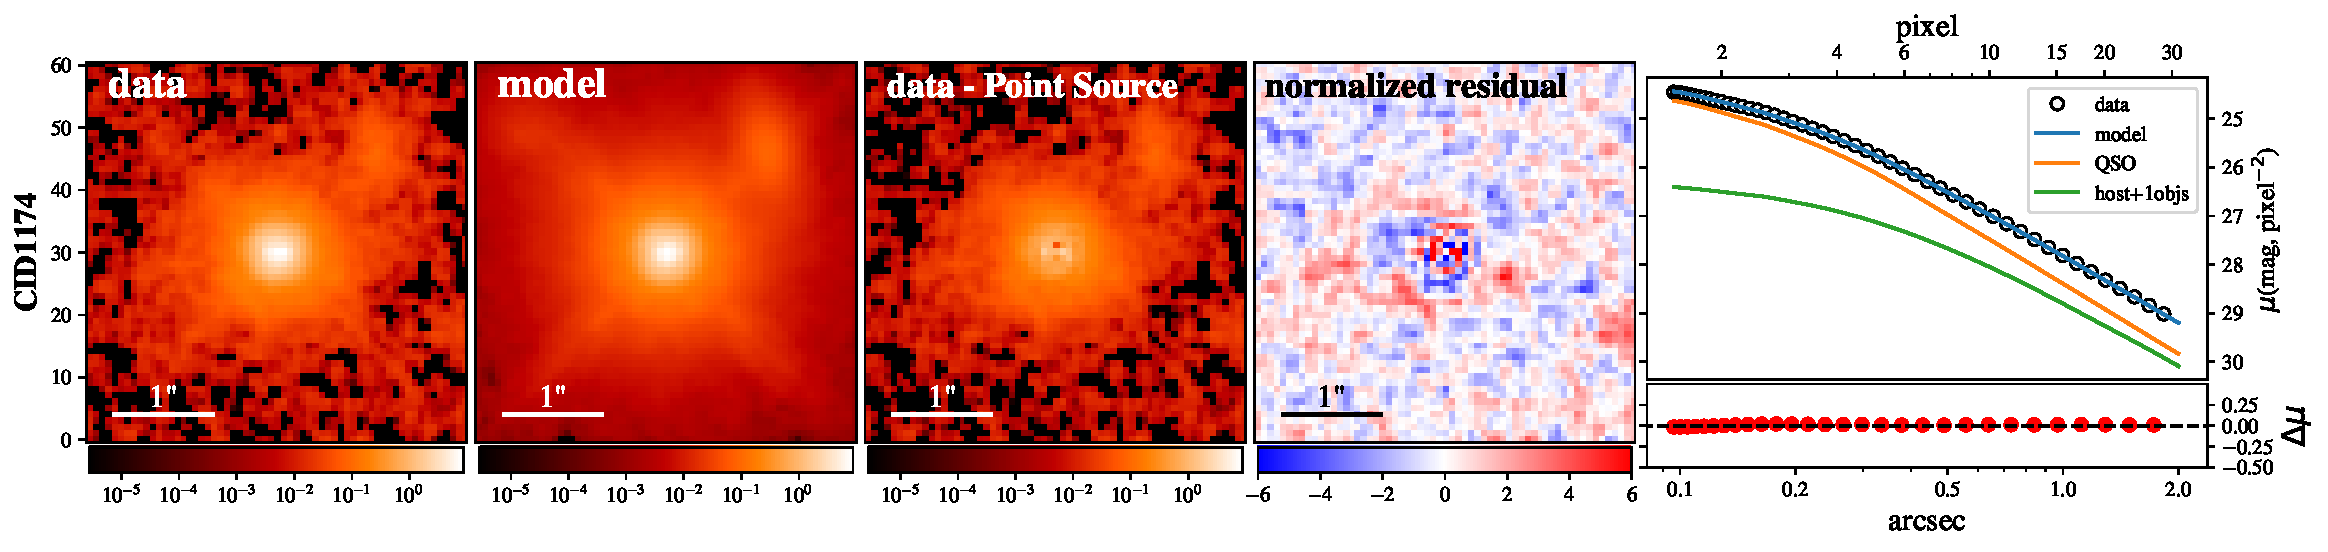
\includegraphics[height=0.25\textwidth]{fig/best_fit_CID1174_SB_profile.pdf}
\caption{\label{fig:AGN_decomp} 
Figure illustrates the inference for the 32 objects based on the WFC3 images.
In each row, observed data (first column), best-fit models (second column), data subtracted by the inferred point source (third column),  normalized residuals (fourth column) are presented together with the target ID. In the fifth column, we present the 1-D surface brightness profiles (top) and the corresponding residual (bottom). The 1-D profiles indicate the surface brightness including the data (open circles), the best-fit model (blue line), the AGN (orange line), and the model for the extended sources (green line, i.e., host and other objects). Note that the one-dimensional surface brightness profiles are only for illustration purposes. The actual fitting is based on the two-dimensional images. The remaining 31 objects of the sample are shown in appendix A.
}}
\end{figure*} 

\begin{deluxetable*}{ccccccc}
\tablecolumns{7}
\tablewidth{0pt}
\tablecaption{Host inference of CID1174} 
\tablehead{ 
\colhead{PSF rank} &
\colhead{total $\chi ^2$} & 
\colhead{weights $w_i$} &
\colhead{host flux (counts)} &
\colhead{host flux ratio}&
\colhead{\Reff (arcsec)}&
\colhead{\sersic\ $n$}
 \\ 
\colhead{(1)} &
\colhead{(2)} &
\colhead{(3)} &
\colhead{(4)} &
\colhead{(5)} &
\colhead{(6)} &
\colhead{(7)} 
} 
\startdata
%\multicolumn{5}{c}{Sample presented in \citet{Treu+07}}\\
%\\
1 & $8584.429$ & $1.000$ & $82.2$ & $35\%$ & $0\farcs{}345$ & $1.1$ \\
2 & $8646.711$ & $0.920$ & $99.1$ & $42\%$ & $0\farcs{}298$ & $1.9$ \\
3 & $8816.947$ & $0.734$ & $76.7$ & $33\%$ & $0\farcs{}365$ & $1.1$ \\
4 & $9304.841$ & $0.383$ & $128.6$ & $55\%$ & $0\farcs{}231$ & $2.8$ \\
5 & $9652.575$ & $0.241$ & $187.5$ & $79\%$ & $0\farcs{}116$ & $6.2$ \\
6 & $9917.101$ & $0.170$ & $100.2$ & $42\%$ & $0\farcs{}287$ & $2.1$ \\
7 & $10018.324$ & $0.148$ & $75.1$ & $32\%$ & $0\farcs{}365$ & $1.2$ \\
8 & $10087.456$ & $0.135$ & $79.8$ & $34\%$ & $0\farcs{}358$ & $1.2$ \\
\hline\\
Weighted value & & & $97.322\pm28.336$ & $42\%\pm12\%$& $0\farcs{}309\pm0\farcs{}065$  & $1.9\pm1.3$  \\
\enddata
\label{tab:weight_CID1174}
\tablecomments{
Column~1: Rank of the PSF from the library.
Column~2: Total $\chi ^2$ for the corresponding PSF.
Column~3: Weights for the inference.
Column~4-7: Fitted value for the host flux, host/total flux ratio, effective radius, and \sersic\ index.
For this sample, the inflation parameter $\alpha$ calculated by Eq.~\ref{eq:alpha} is 16.671.
}
\end{deluxetable*}

\begin{figure*}
\centering
{
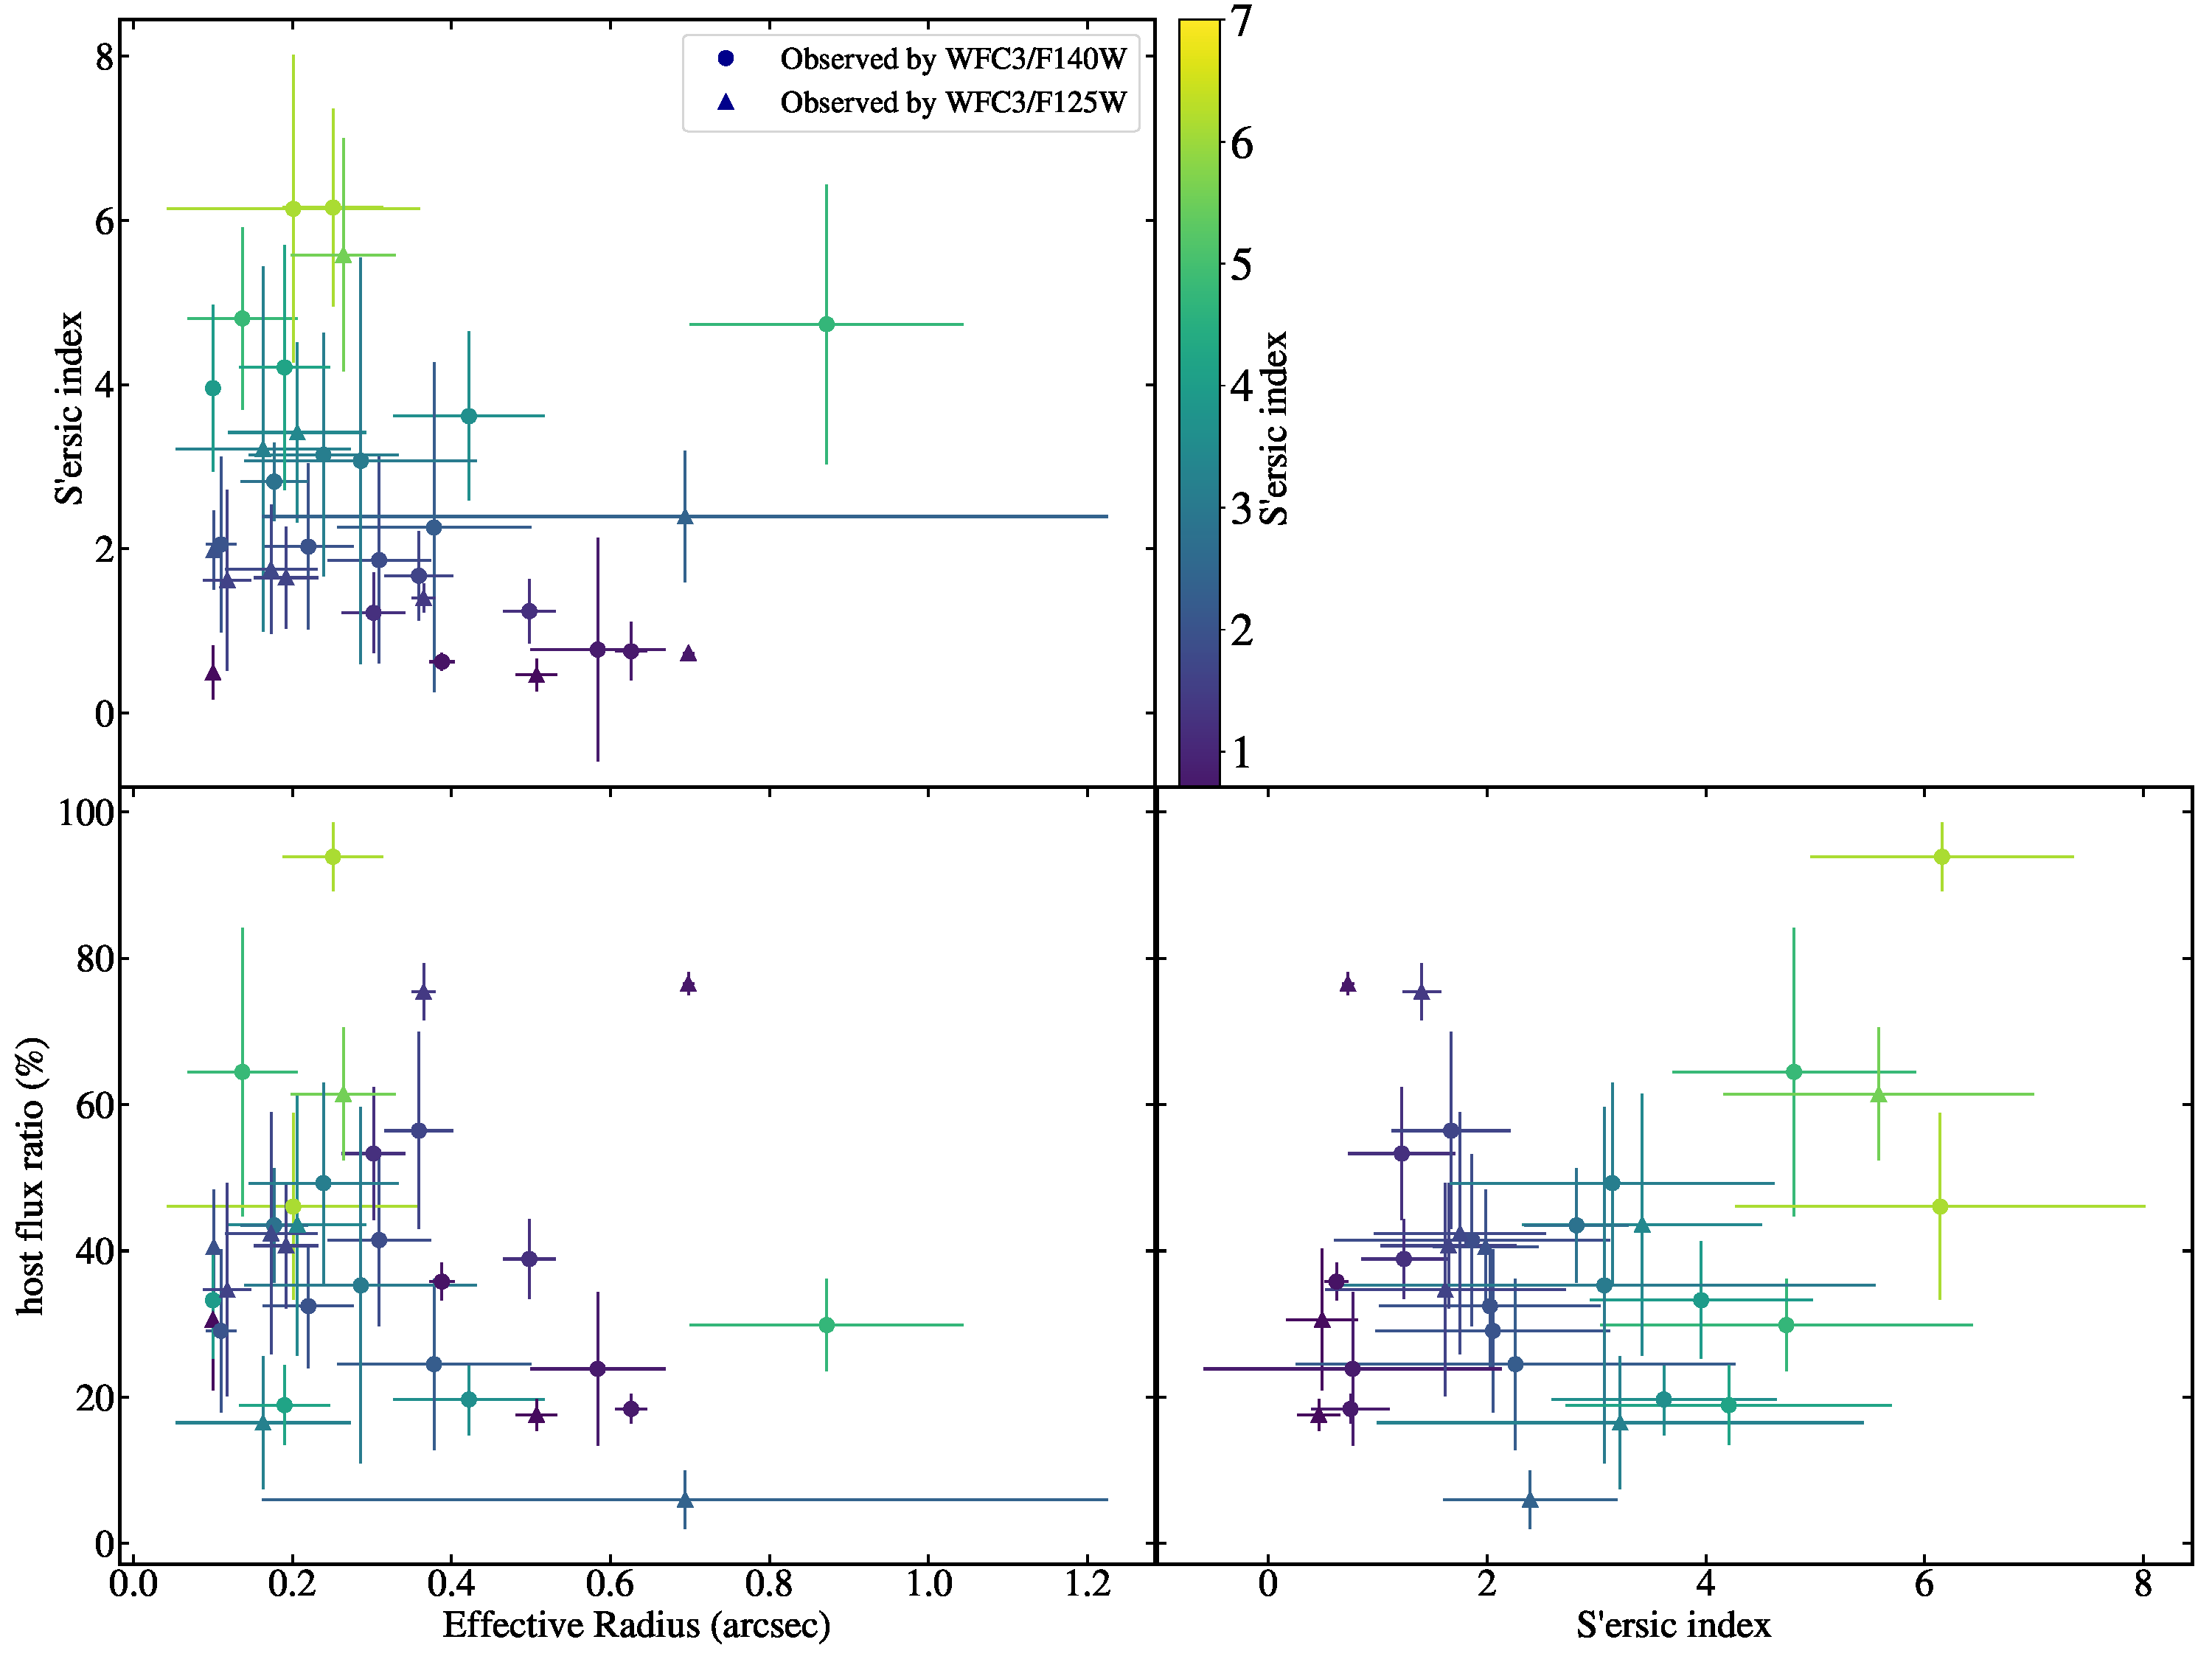
\includegraphics[height=0.75\textwidth]{fig/flux_r_n_corner.pdf}
}
\caption{\label{fig:flux_r_n_corner}
Illustration of the relations between the inferred host \sersic\ parameters.}
\end{figure*} 

The inference of the host properties is weighted by eight top-ranked PSFs. With a smaller amount of PSFs, one would possibly underestimate the uncertainties. To understand how the choice of the number of top-ranked PSF affects our inference, we compare to the inference by five and ten top-ranked PSFs. As shown in Figure~\ref{fig:hist_compare}, the results are very consistent, meaning that the host inference has been solid when the amount of selected PSF exceeds five. 

\begin{figure*}
\centering
{
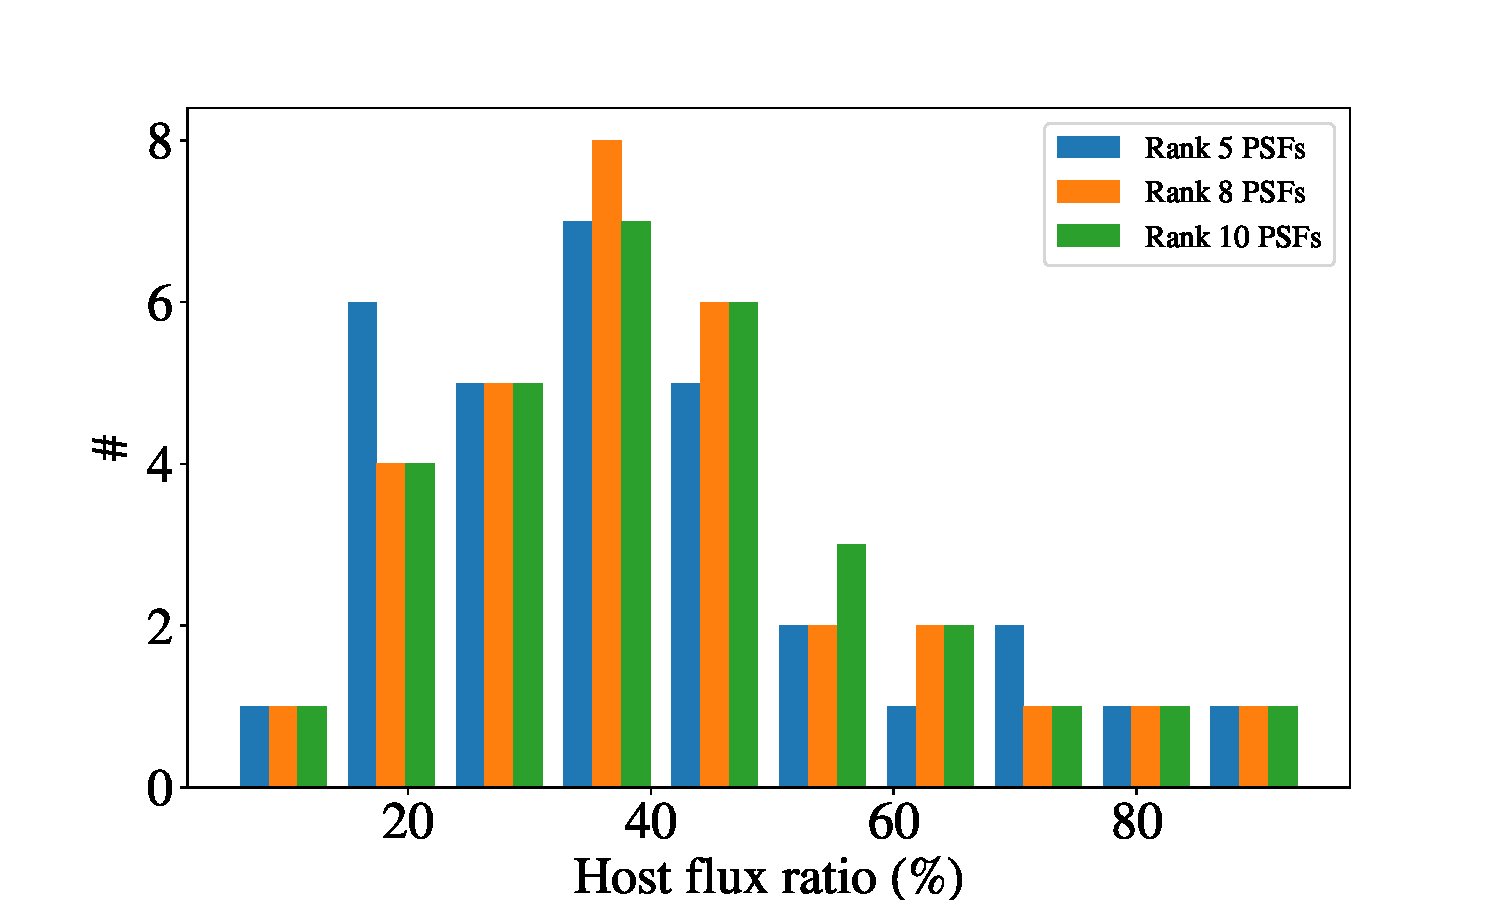
\includegraphics[height=0.35\textwidth]{fig/hist_compare.pdf}
}
\caption{\label{fig:hist_compare} 
Comparison of the histogram of the inferred host flux ratio, based on the different volum of the top-ranked PSFs.}
\end{figure*} 


%The inference of F814w data.
18/32 systems in the COSMOS field have ACS/F184W imaging data. We infer their host flux ratio using the same approach used for the WFC3-IR. The field of view by ACS are larger than WFC3, hence we collected in total 174 ACS PSFs in the library. In principle, the host inference by IR band is superior to the one by UV band, giving that the effects of dust extinction and contrast between the (blue) AGN and (red) host. Thus, we fix the \Reff\ and \sersic\ $n$ as the value inferred by IR band, assuming that the morphology of the galaxy is consistent between ACS and WFC3.

We list all the inference of the host galaxy properties in the Table~\ref{tab:result_sersic}.

\tabcolsep=0.03cm
\begin{deluxetable*}
{@{\extracolsep{4pt}}lcccccccccc}   % need for the gap between the clines.
\tablecolumns{9}
\tablewidth{0pt}
\tablecaption{Inferred host galaxy properties for the 32 systems.} 
\tablehead
{ 
\colhead{Target ID}&
  \multicolumn{5}{c}{WFC3}&
  \multicolumn{3}{c}{ACS/F814W} &
   \multicolumn{2}{c}{host properties} \\
  \cline{2-6}  \cline{7-9} \cline{10-11}  \\
\colhead{}& 
\colhead{reduced $\chi ^2$}& \colhead{host-total flux ratio}& 
\colhead{\Reff}& \colhead{\sersic\ $n$}& 
\colhead{magnitude}&
\colhead{reduced $\chi ^2$}& \colhead{host-total flux ratio}& \colhead{magnitude} &
\colhead{$\log L_R$} &\colhead{$\log M_*$} \\
\colhead{}& 
\colhead{}& \colhead{}& 
\colhead{($\arcsec$)}& \colhead{}& 
\colhead{(AB system)}& \colhead{}& 
\colhead{}& \colhead{(AB system)} &\colhead{($L_{\odot,R}$)} & \colhead{(M$_{\odot}$)}\\
\colhead{(1)}& 
\colhead{(2)}& \colhead{(3)}& 
\colhead{(4)}& \colhead{(5)}& 
\colhead{(6)}& \colhead{(7)}& 
\colhead{(8)}& \colhead{(9)}&
\colhead{(10)}& \colhead{(11)}
}
\setlength{\tabcolsep}{20pt}
\renewcommand{\arraystretch}{1.5}
\startdata 
CID1174 & $2.307$ & $42\%\pm12\%$ & $0\farcs{}31\pm0\farcs{}07$ & $1.9\pm1.3$ & $21.48\substack{+0.37\\-0.28}$ & $2.496$ & $11\%\pm1\%$ & $23.21\substack{+0.11\\-0.10}$ & $11.05\substack{+0.15\\-0.11}$ &$10.78\substack{+0.18\\-0.15}$\\[3pt]
CID1281 & $1.322$ & $49\%\pm14\%$ & $0\farcs{}24\pm0\farcs{}09$ & $3.2\pm1.5$ & $22.88\substack{+0.36\\-0.27}$ & $1.378$ & $19\%\pm8\%$ & $24.83\substack{+0.60\\-0.38}$ & $10.41\substack{+0.15\\-0.11}$ &$10.14\substack{+0.18\\-0.15}$\\[3pt]
CID206 & $2.054$ & $35\%\pm24\%$ & $0\farcs{}29\pm0\farcs{}15$ & $3.1\pm2.5$ & $21.82\substack{+1.30\\-0.58}$ & $1.903$ & $8\%\pm2\%$ & $23.67\substack{+0.40\\-0.29}$ & $10.86\substack{+0.52\\-0.23}$ &$10.59\substack{+0.53\\-0.25}$\\[3pt]
CID216 & $1.514$ & $94\%\pm5\%$ & $0\farcs{}25\pm0\farcs{}06$ & $6.2\pm1.2$ & $21.51\substack{+0.05\\-0.05}$ & $1.425$ & $35\%\pm2\%$ & $23.45\substack{+0.05\\-0.05}$ & $11.05\substack{+0.03\\-0.03}$ &$10.78\substack{+0.10\\-0.10}$\\[3pt]
CID237 & $2.349$ & $30\%\pm6\%$ & $0\farcs{}87\pm0\farcs{}17$ & $4.7\pm1.7$ & $21.28\substack{+0.26\\-0.21}$ & $2.354$ & $3\%\pm2\%$ & $23.72\substack{+1.04\\-0.52}$ & $11.18\substack{+0.11\\-0.09}$ &$10.91\substack{+0.14\\-0.13}$\\[3pt]
CID255 & $1.625$ & $19\%\pm5\%$ & $0\farcs{}19\pm0\farcs{}06$ & $4.2\pm1.5$ & $21.61\substack{+0.37\\-0.28}$ & 2.858 & $4\%\pm2\%$ & $22.89\substack{+0.60\\-0.39} $& $11.08\substack{+0.15\\-0.11}$ &$10.81\substack{+0.18\\-0.15}$\\[3pt]
CID3242 & $2.751$ & $46\%\pm13\%$ & $0\farcs{}20\pm0\farcs{}16$ & $6.1\pm1.9$ & $21.16\substack{+0.35\\-0.26}$ & $2.596$ & $5\%\pm1\%$ & $23.60\substack{+0.34\\-0.26}$ & $11.16\substack{+0.14\\-0.11}$ &$10.89\substack{+0.17\\-0.15}$\\[3pt]
CID3570 & $1.665$ & $77\%\pm2\%$ & $0\farcs{}70\pm0\farcs{}01$ & $0.7\pm0.1$ & $21.16\substack{+0.02\\-0.02}$ & $1.332$ & $86\%\pm2\%$ & $22.97\substack{+0.01\\-0.01}$ & $10.98\substack{+0.02\\-0.02}$ &$10.71\substack{+0.10\\-0.10}$\\[3pt]
CID452 & $1.684$ & $75\%\pm4\%$ & $0\farcs{}37\pm0\farcs{}02$ & $1.4\pm0.2$ & $21.18\substack{+0.06\\-0.06}$ & $1.452$ & $38\%\pm1\%$ & $22.73\substack{+0.02\\-0.02}$ & $11.13\substack{+0.03\\-0.03}$ &$10.86\substack{+0.10\\-0.10}$\\[3pt]
CID454 & $2.203$ & $36\%\pm3\%$ & $0\farcs{}39\pm0\farcs{}02$ & $0.6\pm0.1$ & $21.20\substack{+0.08\\-0.07}$ & $1.291$ & $9\%\pm1\%$ & $23.35\substack{+0.06\\-0.06}$ & $11.11\substack{+0.04\\-0.04}$ &$10.84\substack{+0.10\\-0.10}$\\[3pt]
CID50 & $5.576$ & $17\%\pm9\%$ & $0\farcs{}16\pm0\farcs{}11$ & $3.2\pm2.2$ & $20.93\substack{+0.86\\-0.48}$ & $4.940$ & $5\%\pm3\%$ & $22.50\substack{+1.15\\-0.55}$ & $11.07\substack{+0.35\\-0.19}$ &$10.80\substack{+0.36\\-0.21}$\\[3pt]
CID543 & $1.902$ & $31\%\pm10\%$ & $0\farcs{}10\pm0\farcs{}00$ & $0.5\pm0.3$ & $21.99\substack{+0.41\\-0.30}$ & $1.435$ & $5\%\pm2\%$ & $23.77\substack{+0.53\\-0.36}$ & $10.70\substack{+0.16\\-0.12}$ &$10.43\substack{+0.19\\-0.15}$\\[3pt]
CID597 & $1.565$ & $42\%\pm17\%$ & $0\farcs{}17\pm0\farcs{}06$ & $1.8\pm0.8$ & $21.87\substack{+0.54\\-0.36}$ & $1.254$ & $12\%\pm1\%$ & $23.56\substack{+0.13\\-0.11}$ & $10.73\substack{+0.22\\-0.15}$ &$10.46\substack{+0.24\\-0.18}$\\[3pt]
CID607 & $1.692$ & $44\%\pm18\%$ & $0\farcs{}21\pm0\farcs{}09$ & $3.4\pm1.1$ & $21.19\substack{+0.58\\-0.37}$ & $2.590$ & $5\%\pm2\%$ & $23.57\substack{+0.51\\-0.35}$ & $11.02\substack{+0.23\\-0.15}$ &$10.75\substack{+0.25\\-0.18}$\\[3pt]
CID70 & $2.041$ & $20\%\pm5\%$ & $0\farcs{}42\pm0\farcs{}10$ & $3.6\pm1.0$ & $21.86\substack{+0.30\\-0.24}$ & $2.361$ & $2\%\pm1\%$ & $24.63\substack{+0.68\\-0.41}$ & $10.98\substack{+0.12\\-0.10}$ &$10.72\substack{+0.16\\-0.14}$\\[3pt]
LID1273 & $1.697$ & $53\%\pm9\%$ & $0\farcs{}30\pm0\farcs{}04$ & $1.2\pm0.5$ & $20.94\substack{+0.21\\-0.18}$ & $2.137$ & $6\%\pm1\%$ & $23.29\substack{+0.15\\-0.13}$ & $11.32\substack{+0.09\\-0.07}$ &$11.05\substack{+0.13\\-0.12}$\\[3pt]
LID1538 & $2.362$ & $44\%\pm8\%$ & $0\farcs{}18\pm0\farcs{}04$ & $2.8\pm0.5$ & $21.25\substack{+0.22\\-0.18}$ & $2.173$ & $8\%\pm1\%$ & $23.09\substack{+0.19\\-0.16}$ & $11.12\substack{+0.09\\-0.08}$ &$10.86\substack{+0.13\\-0.12}$\\[3pt]
LID360 & $3.918$ & $18\%\pm2\%$ & $0\farcs{}63\pm0\farcs{}02$ & $0.8\pm0.4$ & $21.46\substack{+0.14\\-0.12}$ & $4.914$ & $4\%\pm1\%$ & $23.25\substack{+0.17\\-0.15}$ & $11.08\substack{+0.06\\-0.05}$ &$10.81\substack{+0.11\\-0.11}$\\[3pt]
XID2138 & $1.597$ & $39\%\pm6\%$ & $0\farcs{}50\pm0\farcs{}03$ & $1.2\pm0.4$ & $21.87\substack{+0.17\\-0.15}$ & $2.731$ & $5\%\pm1\%$ & $23.90\substack{+0.31\\-0.24}$ & $10.89\substack{+0.07\\-0.06}$ &$10.63\substack{+0.12\\-0.12}$\\[3pt]
XID2202 & $3.23$ & $33\%\pm8\%$ & $0\farcs{}10\pm0\farcs{}00$ & $4.0\pm1.0$ & $21.16\substack{+0.30\\-0.24}$ & $3.852$ & $8\%\pm2\%$ & $22.59\substack{+0.29\\-0.23}$ & $11.15\substack{+0.12\\-0.10}$ &$10.88\substack{+0.16\\-0.14}$\\[3pt]
XID2396 & $3.669$ & $24\%\pm11\%$ & $0\farcs{}58\pm0\farcs{}09$ & $0.8\pm1.4$ & $21.40\substack{+0.65\\-0.40}$ & $5.346$ & $2\%\pm1\%$ & $23.36\substack{+0.24\\-0.20}$ & $11.12\substack{+0.26\\-0.16}$ &$10.85\substack{+0.28\\-0.19}$\\[3pt]
CDFS-1 & $1.358$ & $65\%\pm20\%$ & $0\farcs{}14\pm0\farcs{}07$ & $4.8\pm1.1$ & $22.47\substack{+0.40\\-0.29}$ & ... & ... & ... & $10.71\substack{+0.16\\-0.12}$ &$10.45\substack{+0.19\\-0.15}$\\[3pt]
CDFS-229 & $4.329$ & $18\%\pm2\%$ & $0\farcs{}51\pm0\farcs{}03$ & $0.5\pm0.2$ & $21.57\substack{+0.14\\-0.13}$ & ... & ... & ... & $10.90\substack{+0.06\\-0.05}$ &$10.63\substack{+0.12\\-0.11}$\\[3pt]
CDFS-321 & $3.998$ & $25\%\pm12\%$ & $0\farcs{}38\pm0\farcs{}12$ & $2.3\pm2.0$ & $20.34\substack{+0.70\\-0.42}$ & ... & ... & ... & $11.52\substack{+0.28\\-0.17}$ &$11.25\substack{+0.30\\-0.20}$\\[3pt]
CDFS-724 & $1.355$ & $35\%\pm15\%$ & $0\farcs{}12\pm0\farcs{}03$ & $1.6\pm1.1$ & $23.70\substack{+0.58\\-0.38}$ & ... & ... & ... & $10.06\substack{+0.23\\-0.15}$ &$9.79\substack{+0.25\\-0.18}$\\[3pt]
ECDFS-358 & $2.012$ & $56\%\pm14\%$ & $0\farcs{}36\pm0\farcs{}04$ & $1.7\pm0.5$ & $21.34\substack{+0.30\\-0.24}$ & ... & ... & ... & $11.16\substack{+0.12\\-0.10}$ &$10.89\substack{+0.16\\-0.14}$\\[3pt]
SXDS-X1136 & $1.937$ & $41\%\pm8\%$ & $0\farcs{}10\pm0\farcs{}00$ & $2.0\pm0.5$ & $21.92\substack{+0.23\\-0.19}$ & ... & ... & ... & $10.75\substack{+0.09\\-0.08}$ &$10.49\substack{+0.14\\-0.13}$\\[3pt]
SXDS-X50 & $1.423$ & $41\%\pm9\%$ & $0\farcs{}19\pm0\farcs{}04$ & $1.7\pm0.6$ & $21.99\substack{+0.27\\-0.21}$ & ... & ... & ... & $10.80\substack{+0.11\\-0.09}$ &$10.54\substack{+0.15\\-0.13}$\\[3pt]
SXDS-X717 & $1.426$ & $61\%\pm9\%$ & $0\farcs{}26\pm0\farcs{}07$ & $5.6\pm1.4$ & $21.76\substack{+0.18\\-0.15}$ & ... & ... & ... & $10.77\substack{+0.07\\-0.06}$ &$10.51\substack{+0.12\\-0.12}$\\[3pt]
SXDS-X735 & $2.203$ & $32\%\pm9\%$ & $0\farcs{}22\pm0\farcs{}06$ & $2.0\pm1.0$ & $20.92\substack{+0.33\\-0.25}$ & ... & ... & ... & $11.19\substack{+0.13\\-0.10}$ &$10.92\substack{+0.17\\-0.14}$\\[3pt]
SXDS-X763 & $2.376$ & $6\%\pm4\%$ & $0\farcs{}69\pm0\farcs{}53$ & $2.4\pm0.8$ & $24.13\substack{+1.17\\-0.55}$ & ... & ... & ... & $9.95\substack{+0.47\\-0.22}$ &$9.68\substack{+0.48\\-0.24}$\\[3pt]
SXDS-X969 & $1.613$ & $29\%\pm11\%$ & $0\farcs{}11\pm0\farcs{}02$ & $2.1\pm1.1$ & $21.59\substack{+0.52\\-0.35}$ & ... & ... & ... & $11.03\substack{+0.21\\-0.14}$ &$10.76\substack{+0.23\\-0.17}$\\[3pt]
\enddata
\label{tab:result_sersic}
\tablecomments{
Column~1: Object ID.
Column~2-6: WFC3 inference. 
Column~2: Reduced $\chi ^2$ value by the best PSF in the library.
Column~7-9: ACS inference. 
Column~10: Observed host luminosity in the rest-frame R band.
Column~11: Host total stellar mass.
}
\end{deluxetable*}

\section{Results}
\label{sec:result}

\subsection{Host galaxy properties}
We derive the rest-frame R band magnitude ($M_R$) and luminosity ($L_R$) of our sample based on their filter magnitude. 18/32 systems have multi-band host magnitude which enables us to select the best stellar population that could fit the overall sample. We find that the 1~Gyrs stellar population with solar metallicity by Chabrier initial mass function (IMF)~\citep{Bruzual2003} could well match the color between the WFC3 and ACS band magnitude of these samples.

Adopting the color information, we perform the K-correction and derive the rest-frame R band magnitude of our sample. Given that the WFC3 filter we selected is very close to the rest-frame R band, we expect the $M_R$ uncertainty introduced by this K-correction is within 0.05~mag. We derive the rest-frame R band luminosity by $\log L_R/L_{R, \odot} = 0.4 (M_{R, \odot}-M_R)$, where $M_{R, \odot}=4.61$~\citep{Blanton07}.

Taking the stellar population, we estimate the stellar mass content of each host galaxy according to the mass-to-light ratio of the stellar population we adopted. The uncertainty level associated with the stellar mass is expected to be of order 0.1~dex, at fixed stellar initial mass function (changing the initial mass function would change all our stellar masses systematically).


The inferred $L_R$ and $M_*$ are listed in Table~\ref{tab:result_sersic}. In the rest of this section, we compare their relations to the \mbh.

\subsection{\mbh-\lhost\ relation}\label{sec:ml}
We show our measurements of the \mbh-\lhost\ relation together with the comparison sample in Figure~\ref{fig:ML}. Following common practice, we fit the local relation as a linear relation,
\begin{eqnarray}
\label{eq:MLlocal}
\log \big( \frac{\mathcal M_{\rm BH}}{10^{7}M_{\odot}})= \alpha + \beta \log(\frac{L_R}{10^{10}L_{\odot}}),
\end {eqnarray}
which enables direct comparison to the distant sample. The inferred local relations are presented in the Figure~\ref{fig:ML}, showing that the observed \mbh-\lhost\ relation for our measurements is nearly identical to the local and intermediate ones. The observational result shows that the black hole mass and the host luminosity located at a similar relation at different galaxy age.

{\color{blue} 
Considering that both the black hole and host galaxy are expected to evolve over cosmic time, it is essential to transfer high-$z$ measurements to their values at today so as to compare them in an equivalent frame. We will present the discussion of this comparison in Section~\ref{sec:ml-ev}.

\begin{figure}
\centering
{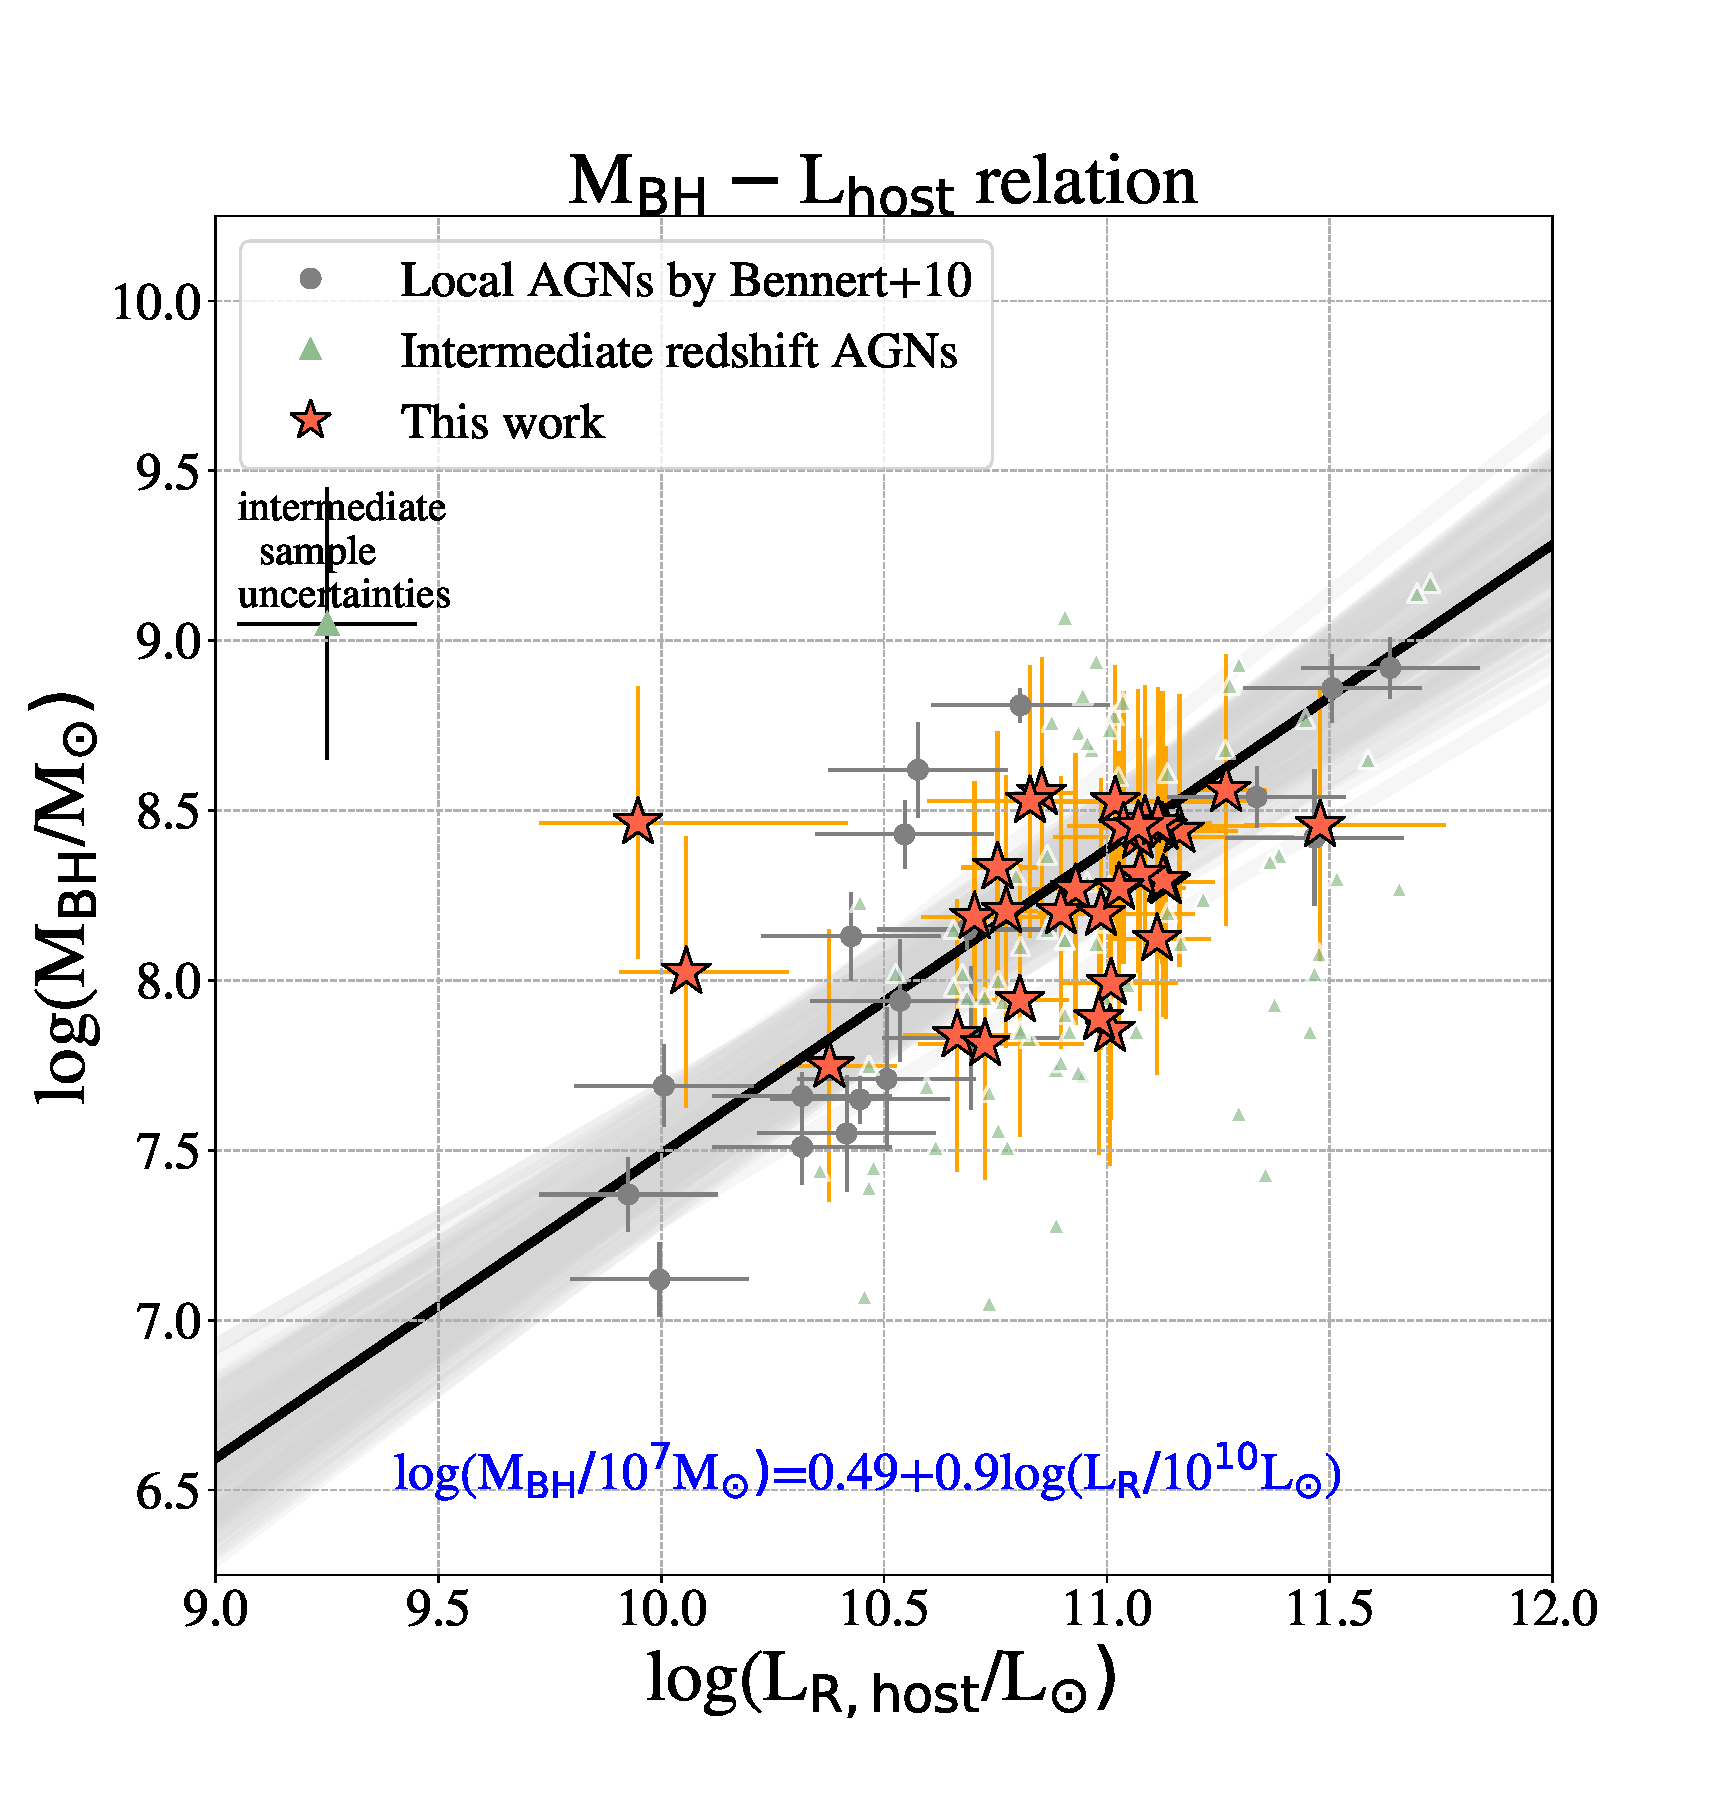
\includegraphics[width=0.5\textwidth]{fig/MBH-L_obs.pdf}}
\caption{\label{fig:ML} 
Illustration of observed correlations between \mbh-\lhost, with local linear relation indicated. 
%The redshift are color-coded, for distant and intermediate AGNs.
The black line and the blue colored equation indicates the best-fit result of local sample as Equation~\ref{eq:MLlocal}, with $1-\sigma$ confidence interval colored as gray region.
}
\end{figure} 

\subsection{\mbh-\smass\ relation}\label{sec:mm}
In Figure~\ref{fig:MM}, we plot the \mbh-\smass\ relation and compare to the local and intermediate sample. We visually see that the relations for the three samples are close from one to another. Similar as Equation~\ref{eq:MLlocal}, we consider the local \mbh-\smass\ relations as linear relation as:
\begin{eqnarray}
\label{eq:MMlocal}
\log \big( \frac{\mathcal M_{\rm BH}}{10^{7}M_{\odot}})= \alpha + \beta \log(\frac{M_*}{10^{10}M_{\odot}}),
\end {eqnarray}

To understand the evolution for high$-z$ relations, we fit the offset as a function of redshift in form as:
\begin{eqnarray}
\label{eq:offset}
\Delta \log \mathcal M_{\rm BH}= \gamma \log (1 + z),
\end{eqnarray} 
where $\Delta \log \mathcal M_{\rm BH} = \log \big( \frac{\mathcal M_{\rm  BH}}{10^{7}M_{\odot}}) -\alpha-\beta\log(\frac{M_*}{10^{10}M_{\odot}})$. We obtain $\gamma  = 0.74 \pm 0.21$, i.e. tentative evidence for evolution, see Figure~\ref{fig:MM-vz}, panel (a). We also show the ratio of \mbh-\smass\ of the three samples at different redshift in Figure~\ref{fig:MM-vz}, panel (b). 

\begin{figure}
\centering
{
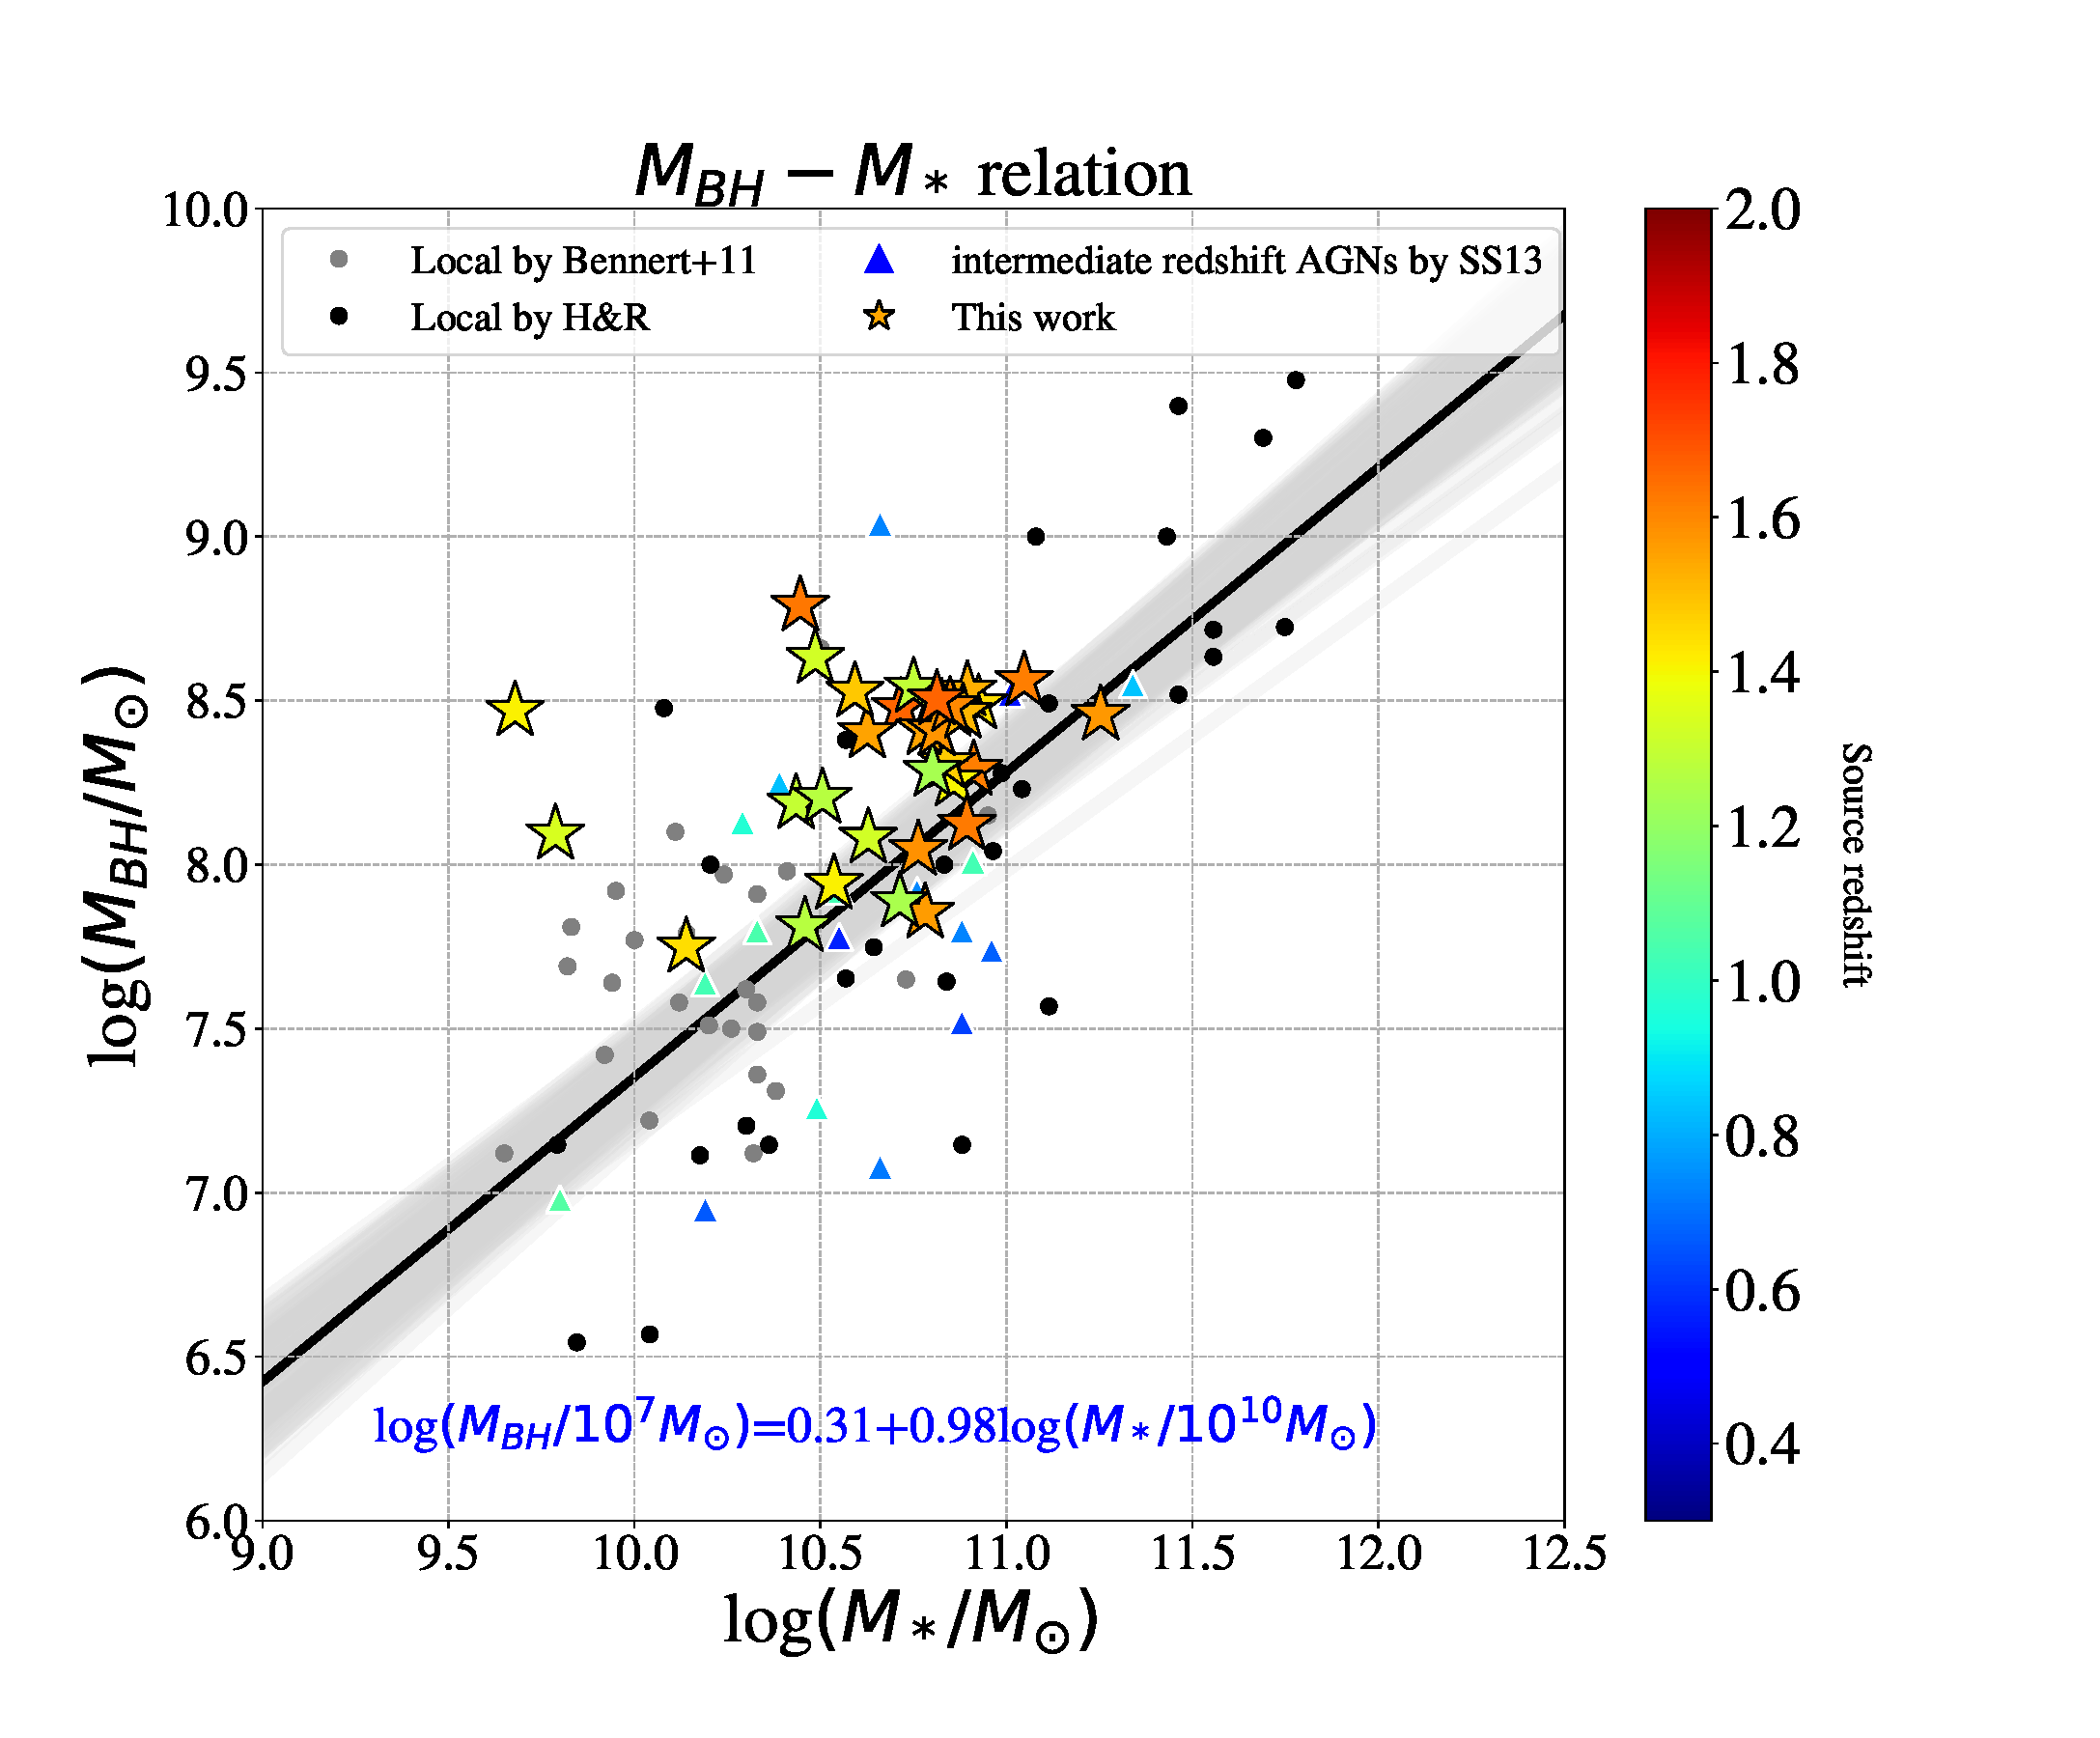
\includegraphics[width=0.5\textwidth]{fig/MBH-Mstar.pdf}
}
\caption{\label{fig:MM} 
Similar to the Figure~\ref{fig:ML}, but the comparison of the \mbh-\smass\ relations.}
\end{figure} 

\begin{figure*}
\centering
\begin{tabular}{c c}
{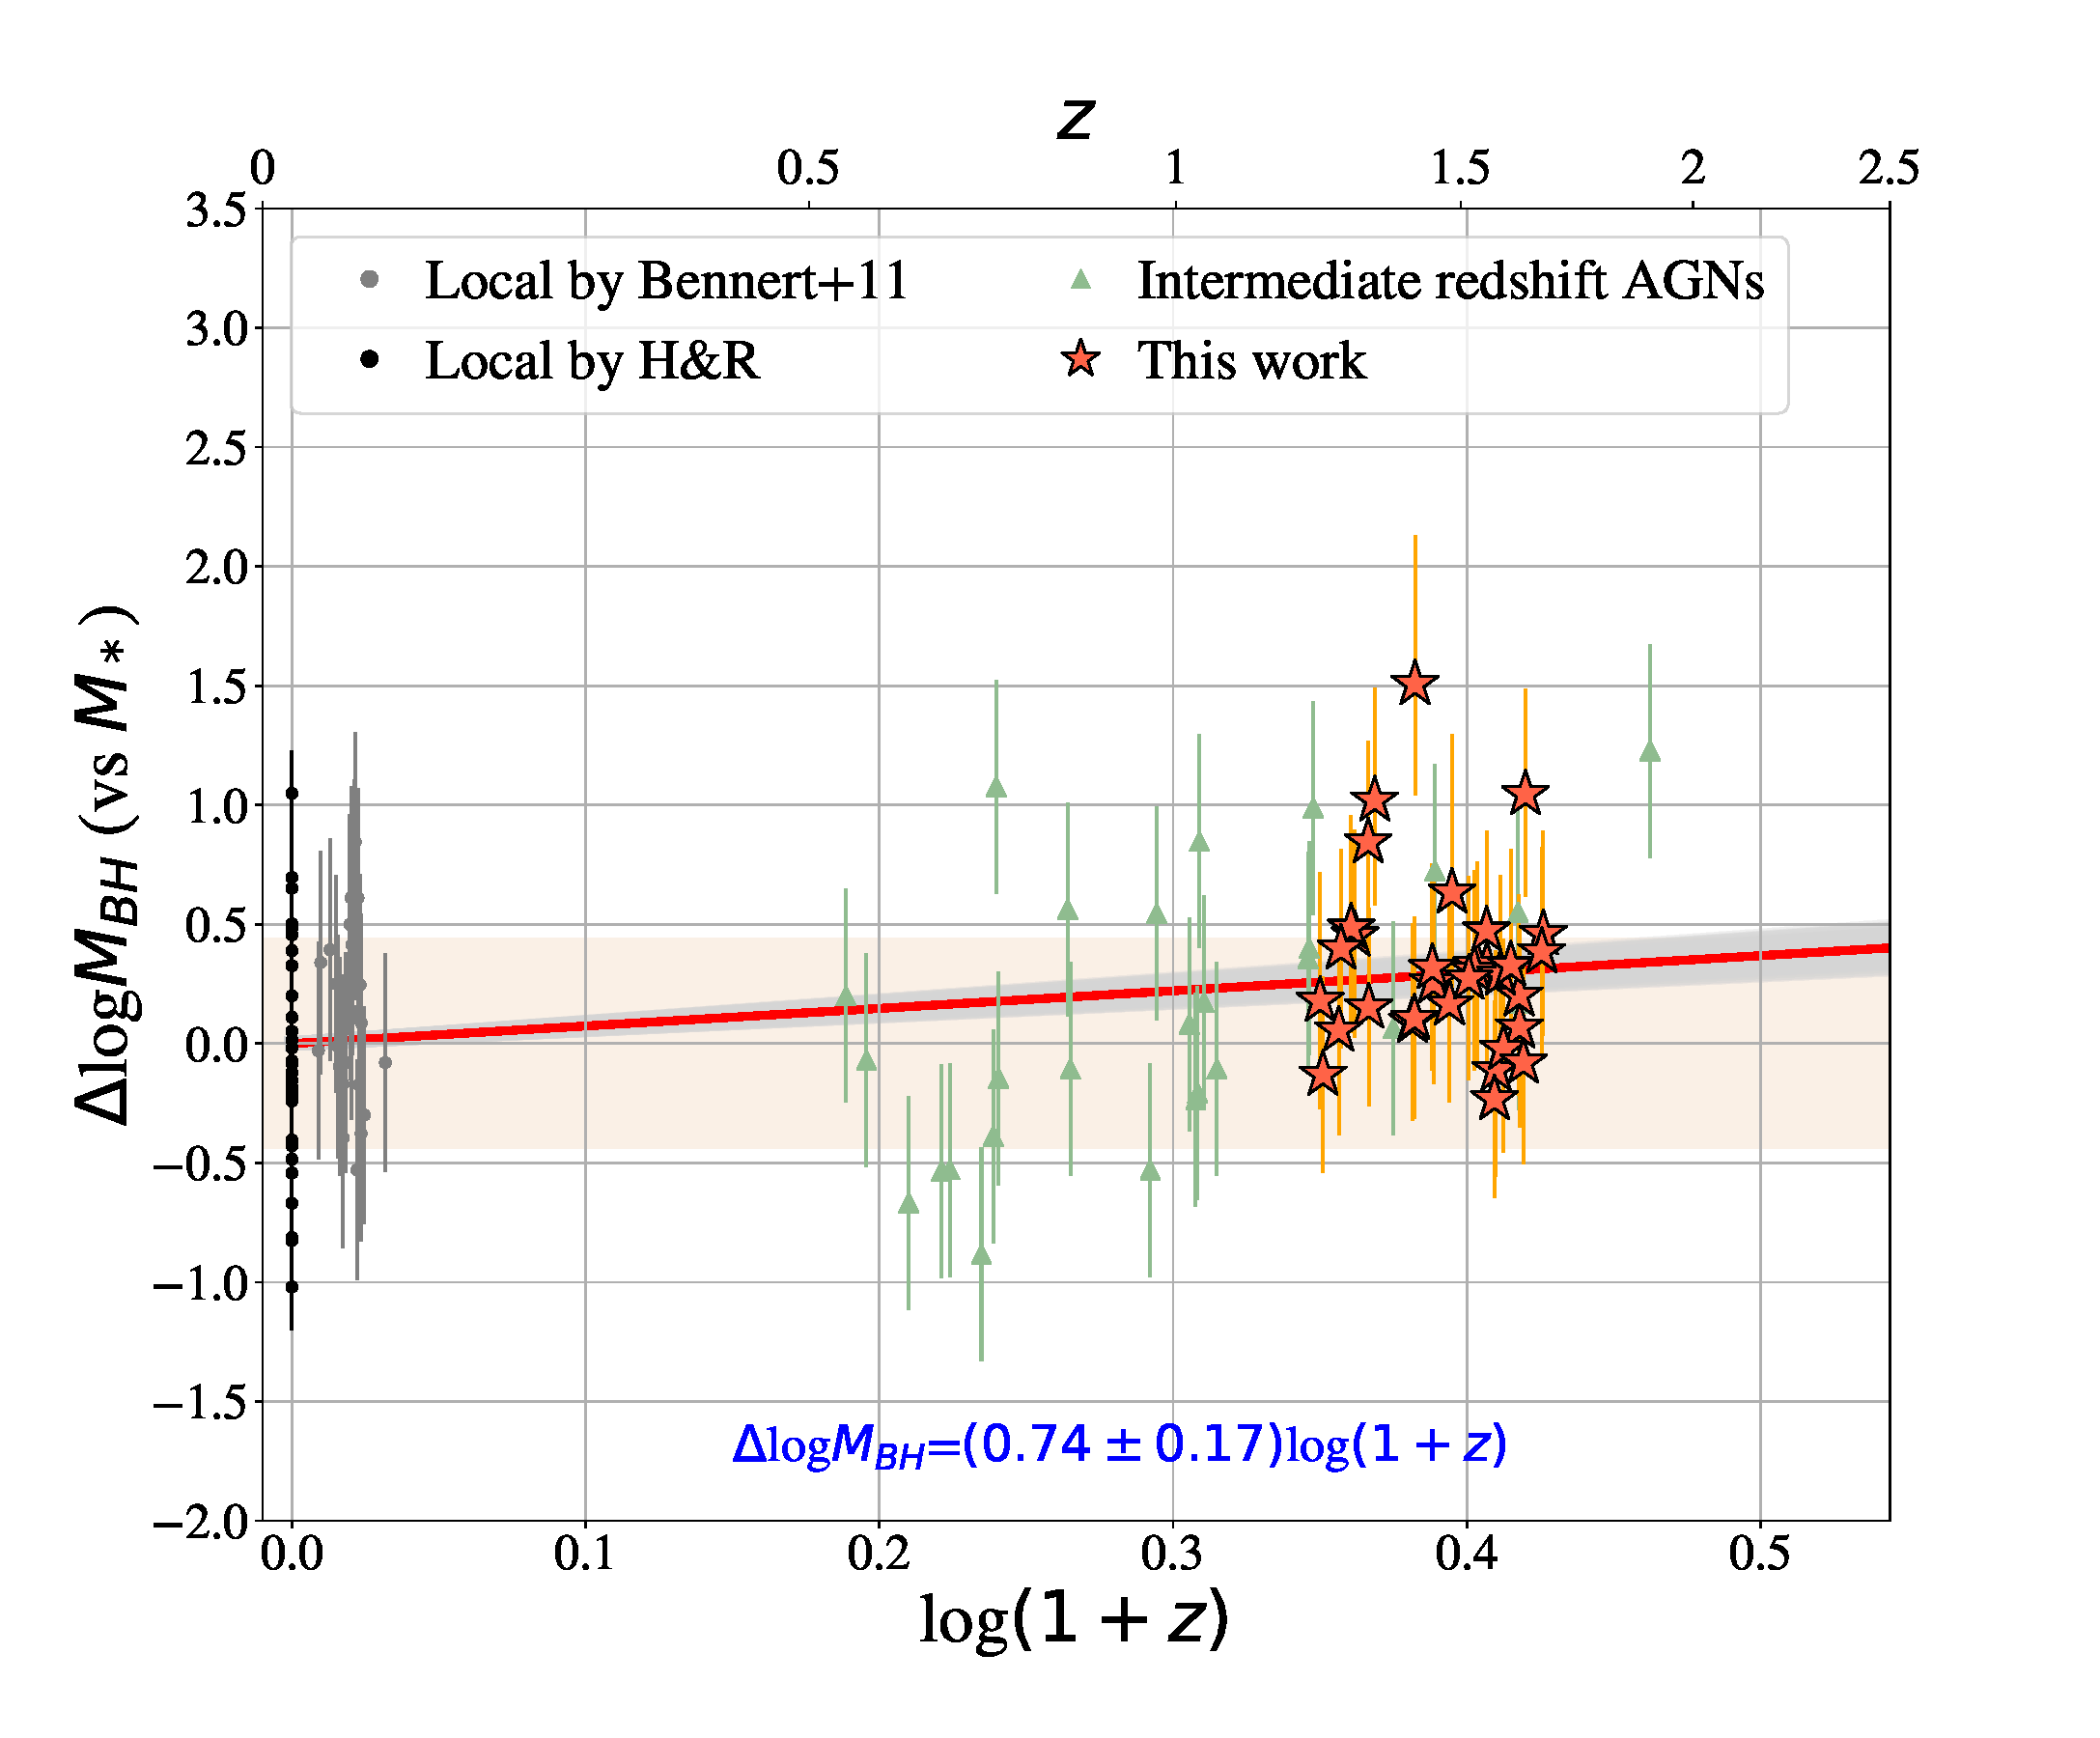
\includegraphics[width=0.5\textwidth]{fig/MBH-Mstar-vz_style1.pdf}}&
{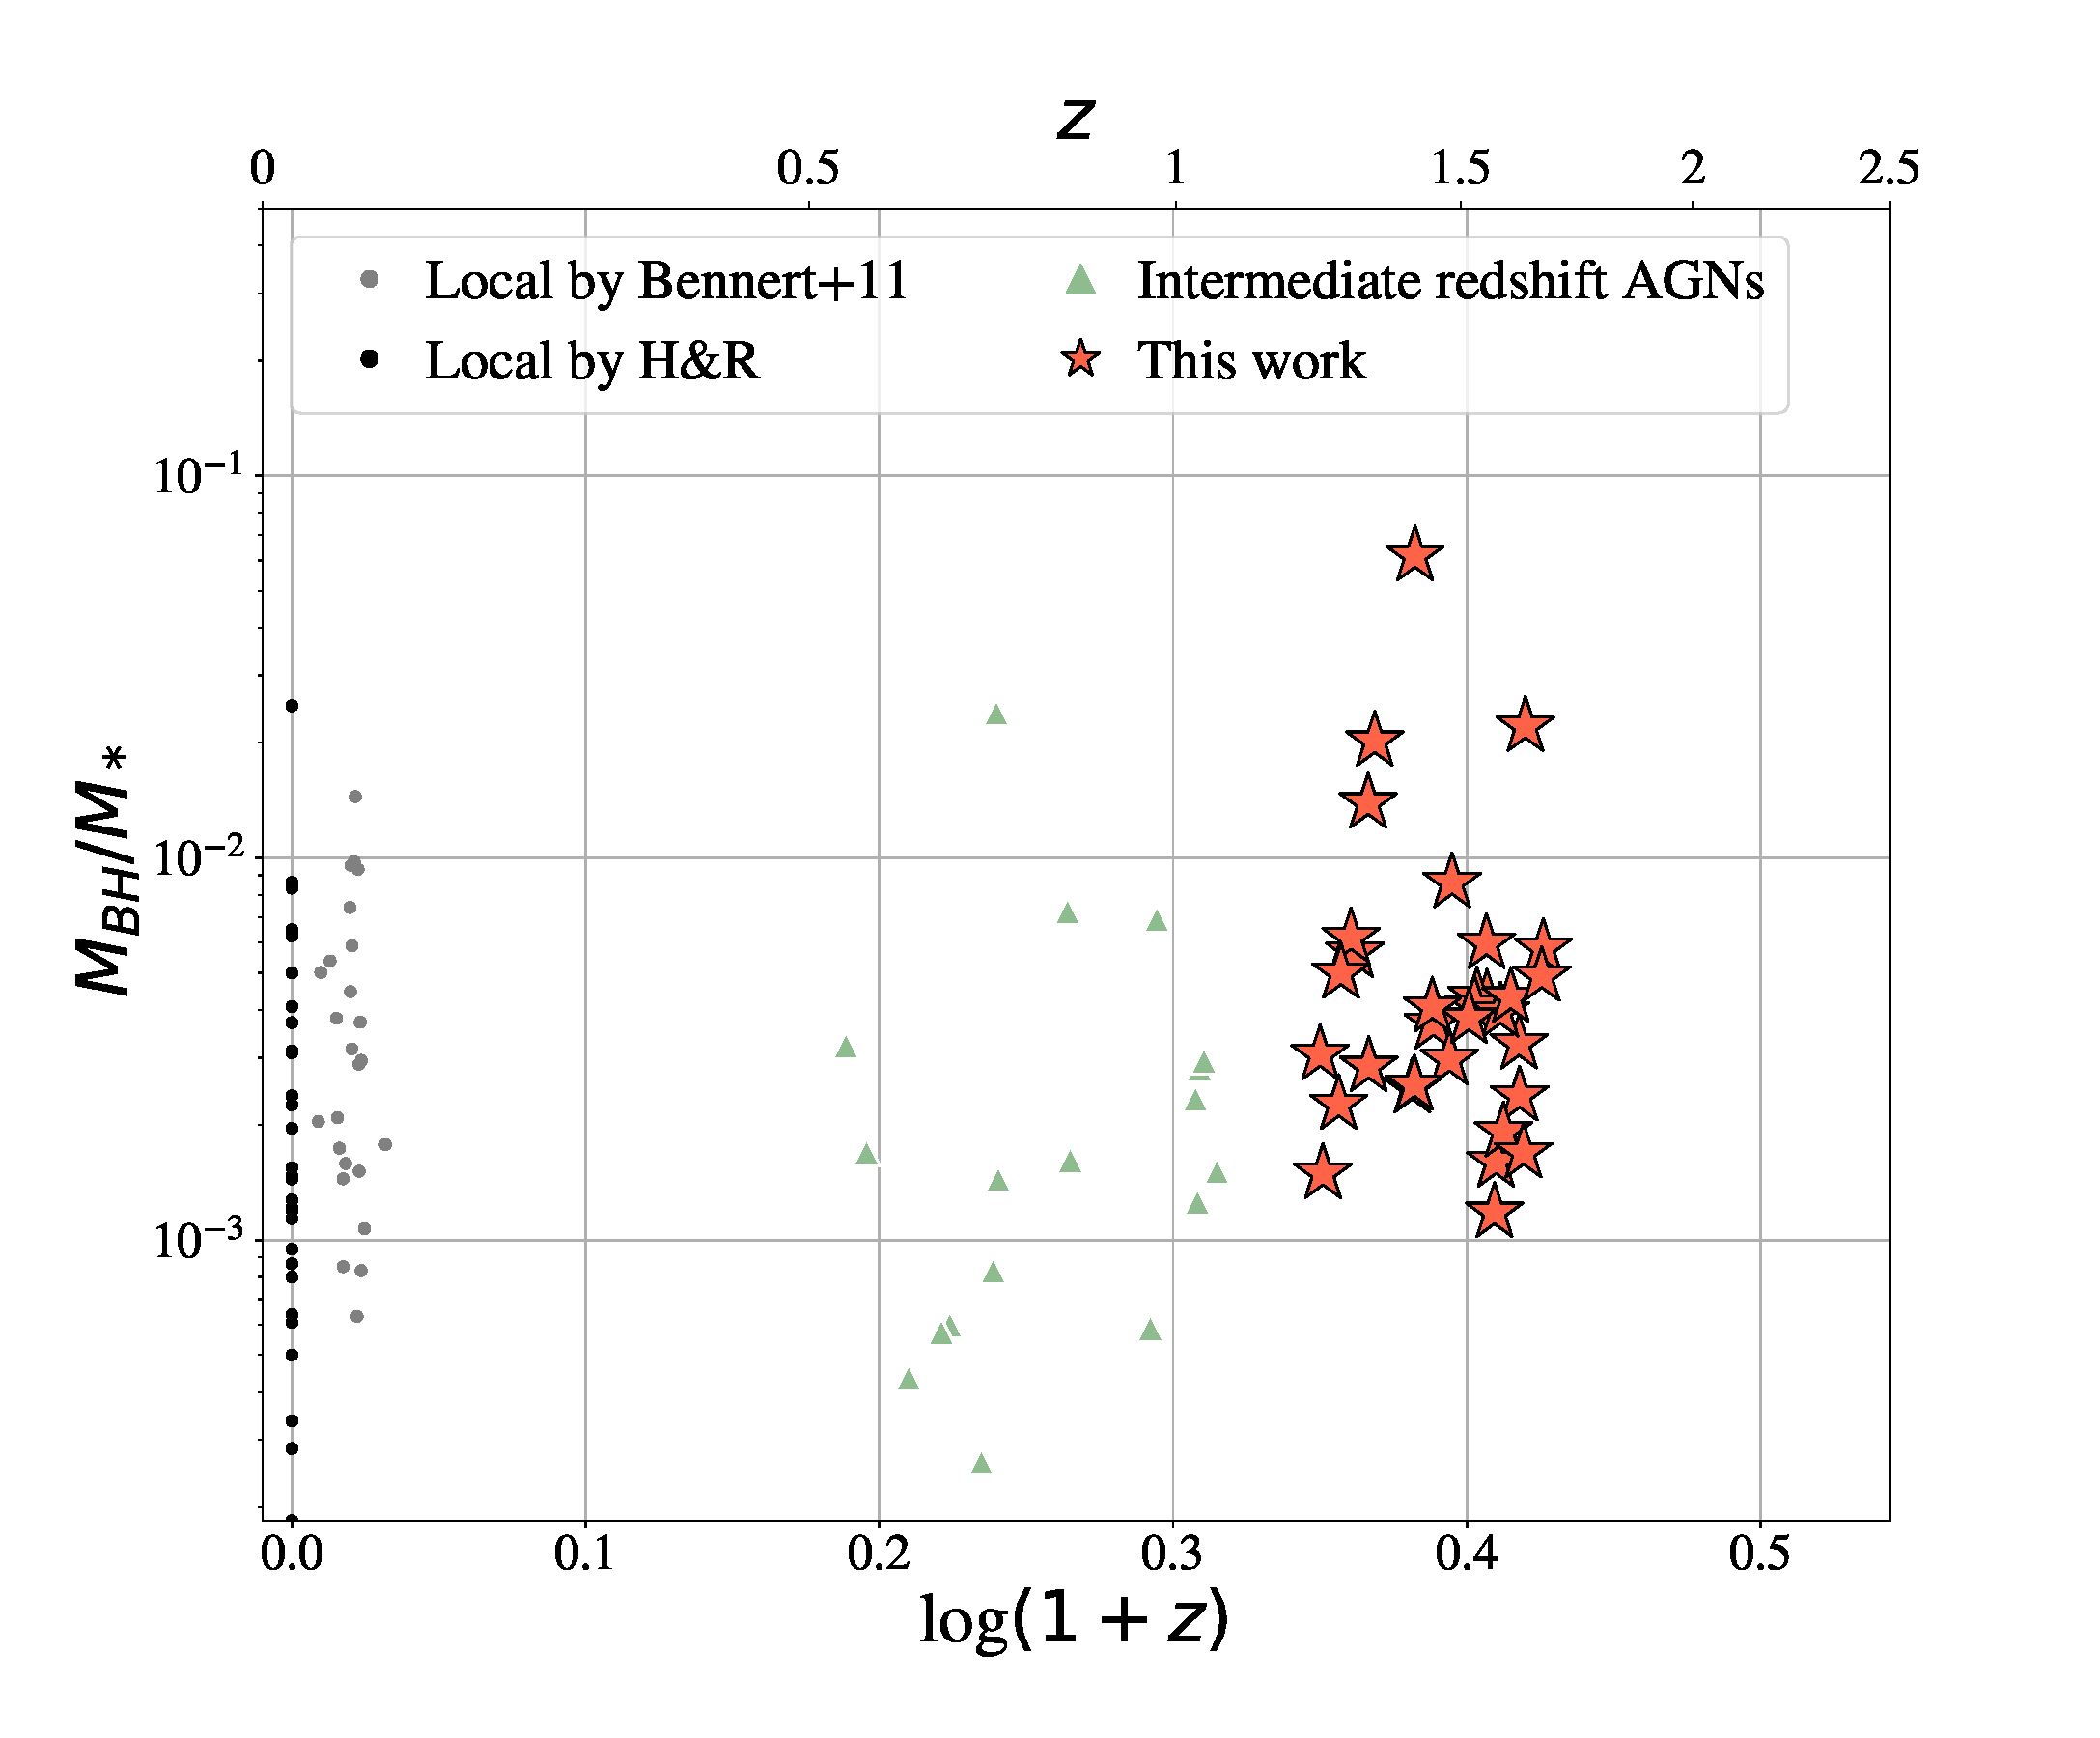
\includegraphics[width=0.5\textwidth]{fig/MBH-Mstar-vz_style0.pdf}}\\
\end{tabular}
\caption{\label{fig:MM-vz} 
Left: illustration of the offset in log\mbh\ (VS. \smass) as a function of redshift. The orange band is the intrinsic scatter of local linear relation. Right: \mbh/\smass\ as a function of redshift.}
\end{figure*} 

We also note that in Figure~\ref{fig:MM-vz}, panel (a), most of our new measurement is visually within the scatter of the local sample. The inference of the positive $\gamma$ seems to stem from the four outliers AGN systems which happens to have lower host mass relative to the BH mass. Thus, we only take the rest of the 28 sample and rerun the statistical analysis, aim to test if offset still exist among them only. As a result, we obtain the $\gamma  = 0.55 \pm 0.29$, indicating a slighter but still positive evolution, i.e. Figure~\ref{fig:MM_restsample}.

\begin{figure}
\centering
{\includegraphics[width=0.5\textwidth]{fig/MBH-Mstar-vz_subsample.pdf}}
\caption{\label{fig:MM_restsample} 
Same as Figure~\ref{fig:MM-vz}, left, but excluding the 4 outliers systems. The result shows the evolution still exist among the other 28 AGN sample.
}
\end{figure} 

It is worth note that the local sample employed are bulge-dominated galaxies and the adopted \smass\ are equivalent to their bulge masses. That is, we are comparing the \mbh-\smass$_{,total}$ at the distant universe to the \mbh-\smass$_{,bulge}$ at the local. Considering that a major part of the distant systems has indicated the disk component (i.e., the systems with fitted \sersic\ index close to 1), the \smass$_{,bluge}$ of them are supposed to be even less.

Without taking into account the selection effect, the direct comparison shows that the growth of the black hole predates that of the host bulge.

\subsection{Selection effect}
\label{select_eff}

Our AGN sample is manually selected based on the mass of BH, the Eddington rates, and \halpha\ broad emission line, with low nuclear-to-host ratios. When adopting the inference from the selected sample to the overall sample without properly considering the selection effect, bias could be introduced~\citep{Tre++07, Bennert++2011, Schulze2014, Park15}. In theory, the simulation~\citep{DeG++15} also find the scaling relations by the selected samples have steeper feature than the random ones, highlighting the necessity of eliminating the selection biases. 

We take selection effects into account using the Monte Carlo simulation based on the approach introduced by \citet{Tre++07}. Following \citet{Park15, Ding2017b}, we generate the simulating samples from a combination of the local active \mbh\ function by \cite{Schulze2010} and the local samples adopted in this work. We then added Gaussian random noise to the simulated samples as a function of two free parameters, $\gamma$ and \sint, where \sint\ is the intrinsic scatter when considering the scaling relation as linear. According to the observed distribution, we consider the observational selection of \mbh\ of our samples by lower and upper limits of $[7.7, 8.8]$ to model their distribution. To evaluate the posterior at the given $\gamma$ and \sint, for each object, we consider the likelihood of observing such object using the simulated sample, and consider whether the object would be selected or not, given the sensitivity. In addition, we adopt both uniform (flat) prior and lognormal prior for \sint\ (using the inference from linear fitting).

Combining the 32 AGNs together with the intermediate redshift sample, we present the inferred  $\gamma$ and \sint\ in the two-dimensional planes in Figure~\ref{fig:select_effect}. With a lognormal prior for \sint, the fitted $\gamma = 0.8\pm0.3$, consistent with the inference by the flat prior. These inference are consistent with the previous values without considering the selection effect in Section~\ref{sec:mm}, indicating that the evolution feature of our sample exist globally in the overall samples. Furthermore, we find that the final inferred scatter \sint$\sim 0.3$ are similar to the local scatter, suggesting that the scatter of the scaling relation at high redshift are similar to local ones and indicating that we have not significantly underestimated/overestimated our errors for high redshift samples.

We also study the selection effect by only consider the new 32 AGNs, result in a higher evolution trend with a higher value of $\gamma$. We show all the result of the $\gamma$ and \sint\ in Table~\ref{table:gamma_sf}.

\begin{table}
\centering
    \caption{The summary for the different inference of $\gamma$.}\label{table:gamma_sf}
     \resizebox{8cm}{!}{
     \begin{tabular}{cccc}
     \hline
     Sample & Selection effects &  \mbh-\smass & \mbh-\lhost \\
     &&&\\
     \hline\hline
32 AGNs + intermediate & No & 0.74$\pm$0.21 & 0.70$\pm$0.18 \\
32 AGNs + intermediate& Yes & 0.80 $\pm$ 0.30 & 0.60 $\pm$ 0.30 \\
32 AGNs & No & 0.80$\pm$0.27  & 1.13$\pm$0.23\\
32 AGNs& Yes & 1.30$\pm$0.50 & 1.70$\pm$0.40 \\
     \hline
     \end{tabular}}
    \tablecomments{
    Entire sample includes the 32 AGNs and the intermediate redshift AGNs from the reference in Section~\ref{sec:compare_sample}. Note that the adopted \lhost\ have been transferred to today assuming the passive evolution scenario using Equation~\ref{eq:L_relation}.
The results of selection effects used the lognormal prior of \sint.
}
\end{table}

\begin{figure*}
\centering
\begin{tabular}{c c}
\subfloat[\mbh-\smass, flat prior]
{\includegraphics[width=0.5\textwidth]{fig/MM_MC_seleff_flatprior.pdf}}&
\subfloat[\mbh-\smass, lognormal prior]
{\includegraphics[width=0.5\textwidth]{fig/MM_MC_seleff_lognormprior.pdf}}\\
\end{tabular}
\caption{\label{fig:select_effect} 
Constraining the evolution factor $\gamma$ of \mbh-\smass\ relation using Equation~\ref{eq:offset}, with intrinsic scatter \sint, using Monte Carlo simulation, by taking selection effects into account. The adopted sample includes 32 AGNs and the intermediate redshift AGNs, using flat prior of \sint\ (left panel) and lognormal prior (right panel).
}
\end{figure*} 

\section{discussion}
\label{sec:dis}

\subsection{Host luminosity passive evolution correction}\label{sec:ml-ev}
In a passive evolution scenario, we expect \lhost\ to fade over time. We transfer the \lhost\ for distant samples at today and compare them to the local in an equivalent frame 

We consider this scenario following \citet{Ding2017b} and parametrize the luminosity evolution with the functional form as
$d{\rm mag}_{\rm R} \sim d\log(1+z)$, i.e.,
\begin{eqnarray}
\label{eq:L_relation}
\log(L_{R,0})=\log(L_{R}) - 1.48 \log (1+z).
\end{eqnarray} 
This formalism is more accurate to fit a broad range redshift comparing to a single slope as $d$mag$/dz$. We refer to \citet[][section 5.4]{Ding2017b} for more details.

We find that, as showing in Figure~\ref{fig:ML-vz}-(a), after transferring the \lhost\ to today, at fixed \mbh, the BH in the more distant universe tends to reside in less luminous hosts, which is consistent to the \mbh-\smass\ relation. To quantitatively understand this trend, we fit the offset as a function of redshift in form following Equation~\ref{eq:offset}. The best-fit and 1-$\sigma$ inference are $\gamma = 0.71 \pm 0.18$, i.e.  Figure~\ref{fig:ML-vz}-(b). We consider the selection effect use the same approach as introduced in Section~\ref{select_eff}, and obtain $\gamma = 0.6\pm0.3$ with lognormal prior, showing in Figure~\ref{fig:ML-vz}-(c), (d).

This section is based on a simplified correction, after all we are not clear exactly how they were evolving to $z=0$. Also, we only consider the evolution of the host galaxy but not the BH. Thus, the correlation of the \mbh-\smass\ would be more efficient to understand the co-evolution connection between BH and its host galaxy.

\begin{figure*}
\centering
\begin{tabular}{c c}
\subfloat[\mbh-\lhost\ relation, evolution-corrected]
{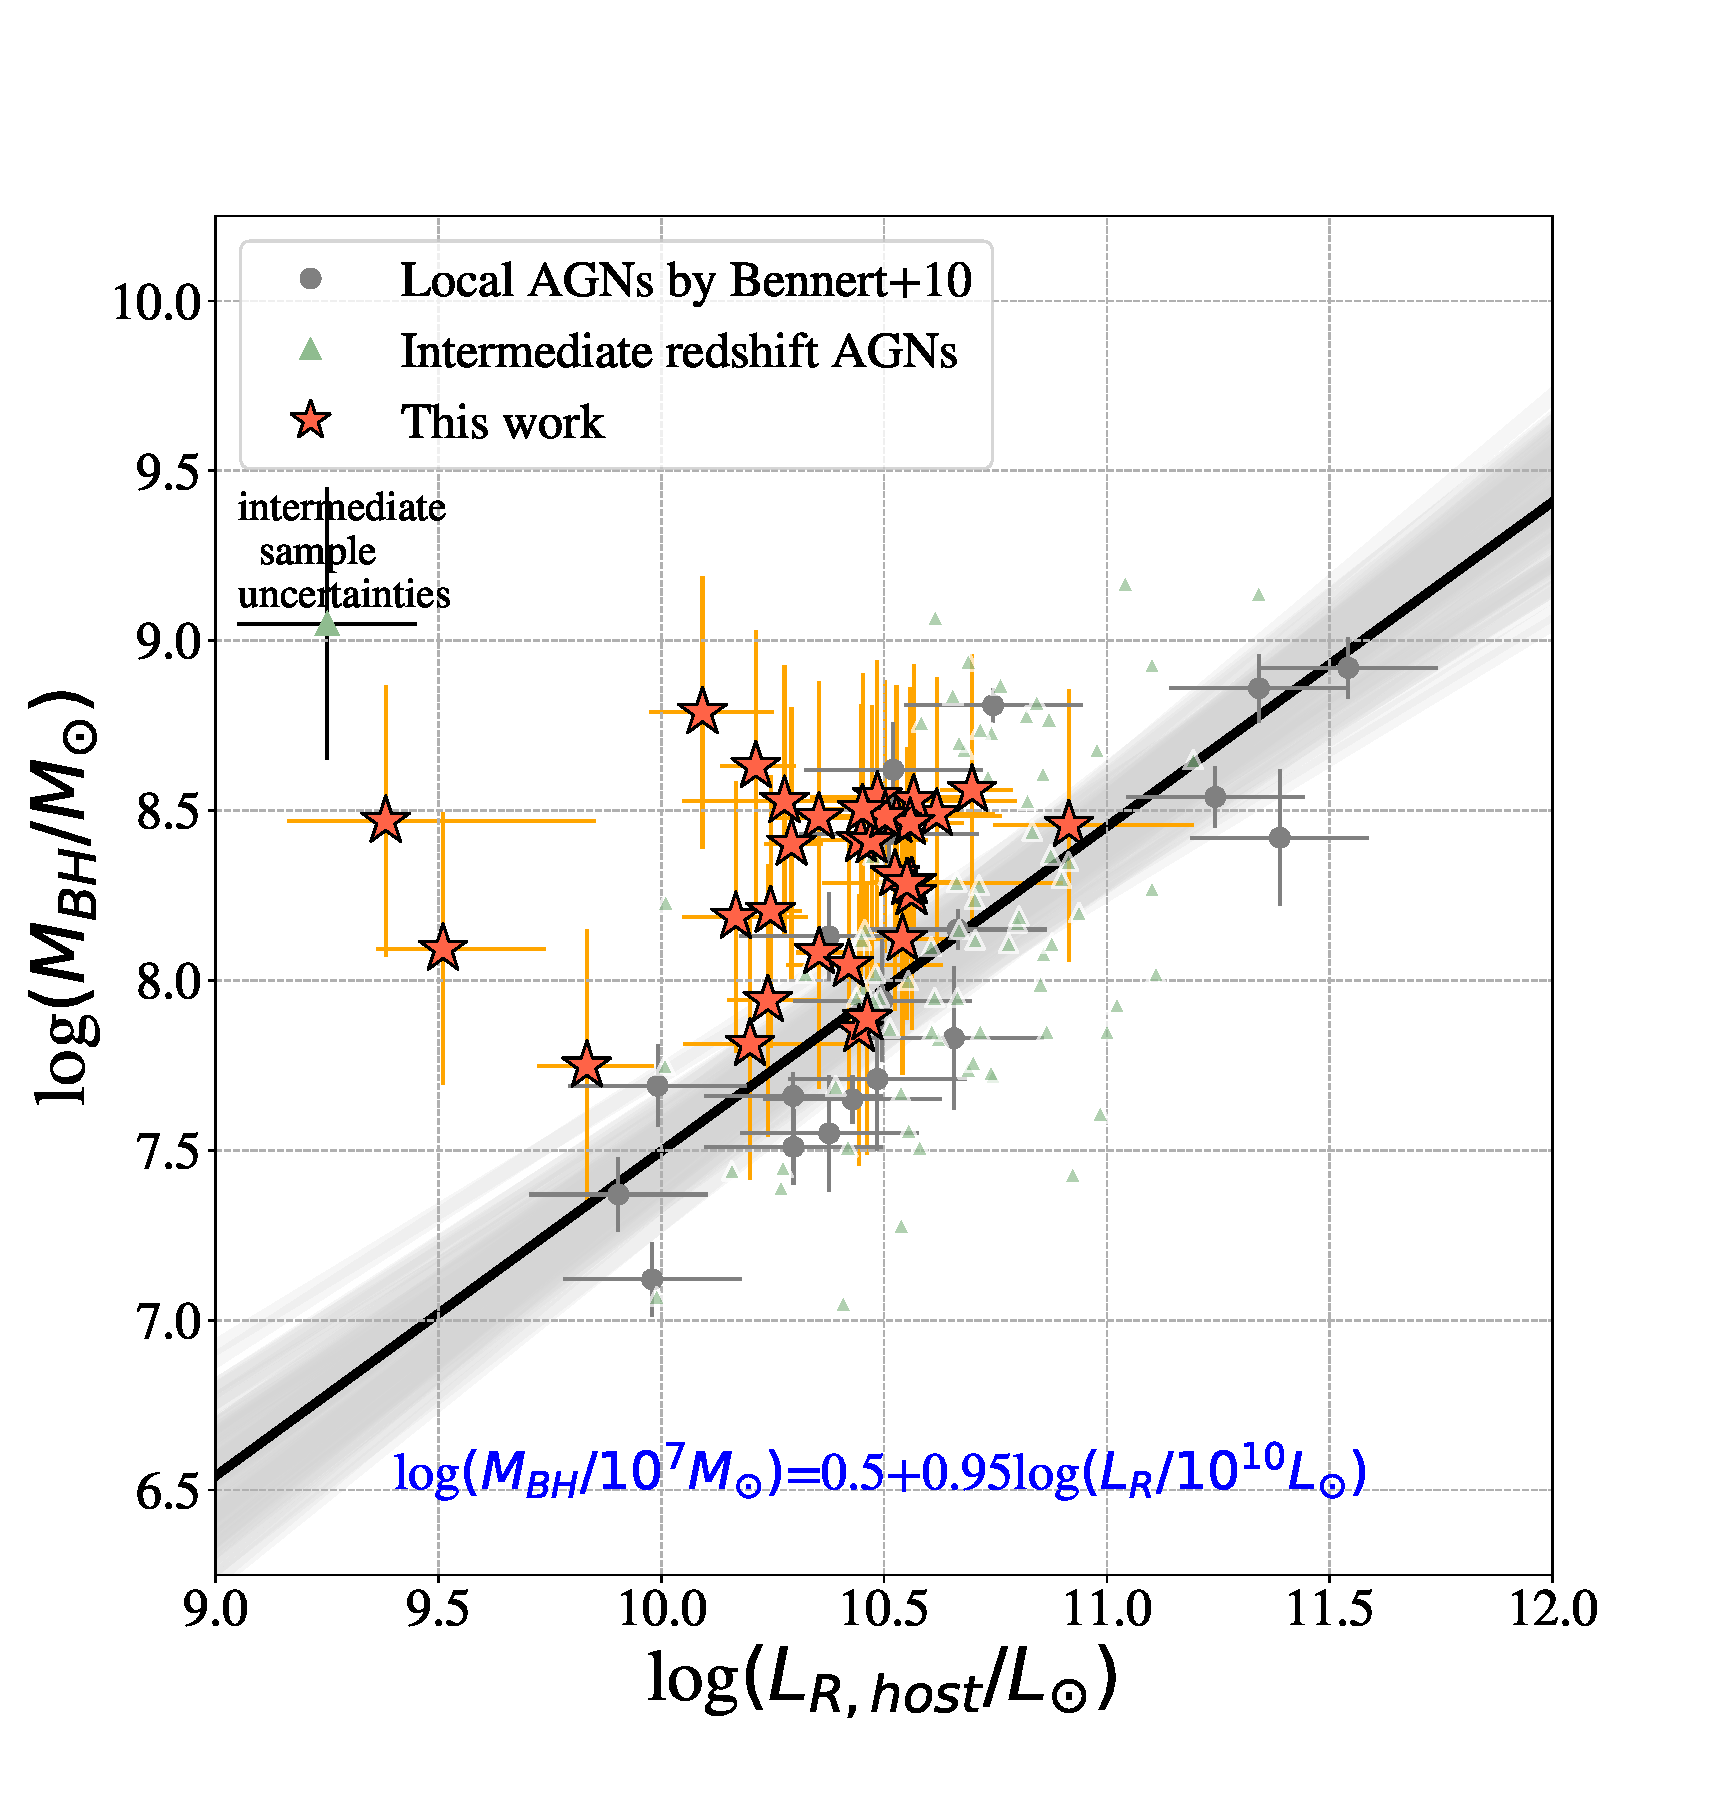
\includegraphics[height=0.4\textwidth]{fig/MBH-L_ev.pdf}}&
\subfloat[offset in log\mbh\ (VS. \lhost) as a function of redshift]
{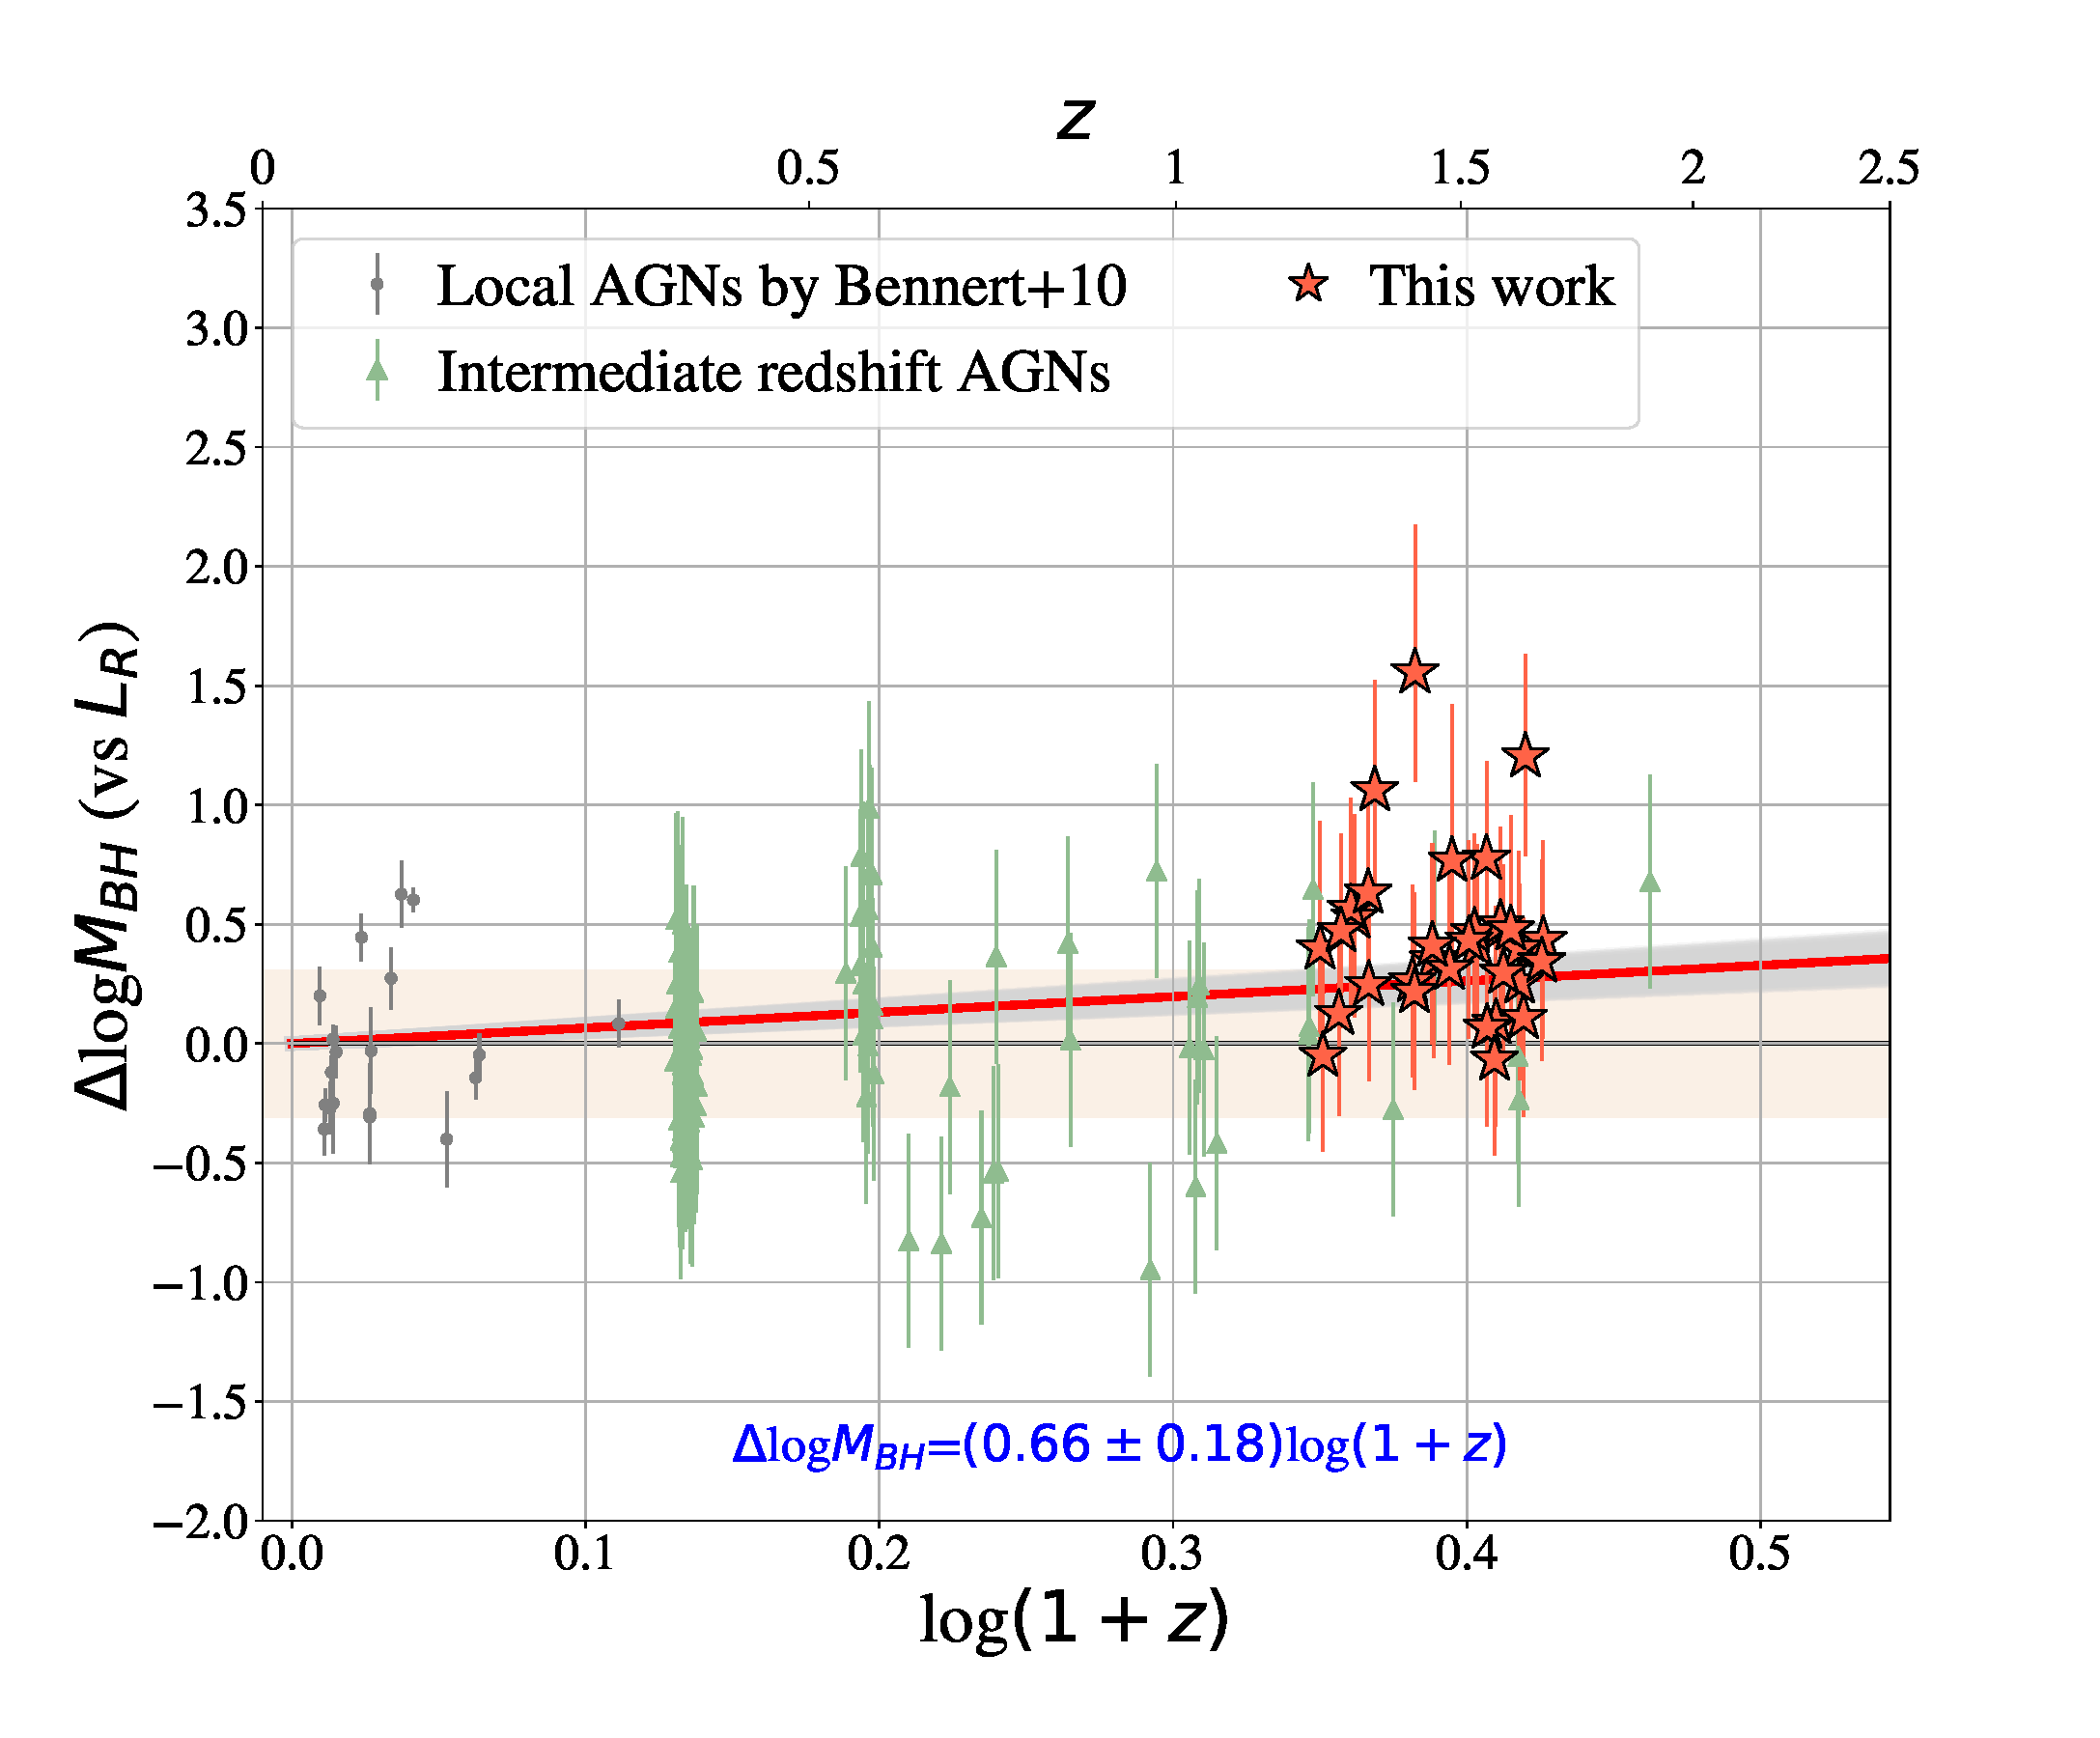
\includegraphics[height=0.4\textwidth]{fig/MBH-L-vz.pdf}}\\
\subfloat[\mbh-\lhost, flat prior]
{\includegraphics[width=0.5\textwidth]{fig/ML_MC_seleff_flatprior.pdf}}&
\subfloat[\mbh-\lhost, lognormal prior]
{\includegraphics[width=0.5\textwidth]{fig/ML_MC_seleff_lognormprior.pdf}}\\
\end{tabular}
\caption{\label{fig:ML-vz} 
Same as previous figures but for \mbh-\lhost relation, considering the passive evolution correction for host galaxy luminosity.}
\end{figure*} 


\subsection{Systematic error}
In this work, we use the start-of-the-art techniques to derive the host flux from the AGN image. The fidelity of the inferred apparent magnitudes of the host galaxies are high. Nevertheless, we adopt one stellar population to the overall sample to derive the rest-frame R band luminosity and stellar mass.
We note that adopting the private stellar populations for each samples which havs both multi-band host magnitude could be more robust in principle. However, considering that the host magnitude in ACS band is faint (host-total flux ratio $< 30\%$), the fidelity of the SED fitting is actually lost. Perhaps the best way to derive the stellar population is to combining our measurements to the ground-based photometry.
We highlight that, in this particular paper, we focus most on the decomposing of the AGN image to present our inference of the host. In the mean time, we carry out a rapid analysis of the \mbh\ and host properties relations. The measurements incorporating the ground-based photometry and the comparison with the simulations are presented in our companion paper.

At last, we stress that the uncertainty in the scaling relations is dominated by the single epoch black hole mass estimates. That is to say, the intrinsic scatter is not necessarily worse at high-$z$ than the low-$z$.

\subsection{Affect using different local anchor}
%Why we local anchor for this paper, for a consistency to the previous work.
%However, the other local samples could be different.
%The comparison of the local MM?
%The corresponding systemic error?
To determining the scaling relations at the local universe, we adopt the local measurements by \citet{Ben++10, Bennert++2011, H+R04}. This adopting enable a direct comparison with the previous work \citep{Park15, SS13}, which adopted the same local sample. We realize that in the literature, there are other local measurements which could shift the local anchor hence affect the conclusion of the co-evolution. For example, we compare our local \mbh-\smass\ sample to the ones by \citet{Kormendy13} (hereafter K13), as showing in Figure~\ref{fig:local_MM_comp}.

We compare the inference of the local linear relation using different combinations of the local sample. It turn out that the inference by HR04+B11 has a lower intercept value to the sample by K13+B11 by 0.3~dex. Apparently, adopting the local by K13+B11 would raise the local relation, hence mitigate the offset of $\Delta\log\mathcal M_{\rm BH}$ and $\gamma$ by a factor of 0.3~dex. Given the values in Table~\ref{fig:MM_restsample}, this mitigating wouldn't affect our inference of $\gamma$ from positive to negative, however, the current offset highlights the importance to build a solid local baseline for the future studies (Bennert et al., in prep).

\begin{figure}
\centering
{\includegraphics[width=0.5\textwidth]{fig/local_MM_comparison.pdf}}
\caption{\label{fig:local_MM_comp} 
The local \mbh-\smass\ relations from different literature. The black and red line are the best-fit linear relation using the sample by combining B11+HR04 and B11+ K13, respectively, showing a 0.3~dex offset in the intercept value.
}
\end{figure} 

\subsection{Comparison to the inactive galaxies}
We compared the morphology of AGNs host galaxies to the inactive galaxies in CANDLES imaging survey. We select 4401 inactive galaxies in a comparable redshift range ($1.2<z<1.7$) whose \sersic\ properties are inferred by \citet{VDwel++2012} by \galfit, and their stellar masses are derived by 3-D-HST spectroscopic survey~\citep{Momcheva2016, Brammer2012}.

In Figure~\ref{fig:Mstar-rn}, we plot the \smass\ versus the \Reff\ and \sersic\ index. The color coding is based on the filter flux ratio between WFC3 and ACS. The distribution of \smass-\Reff\ relation show that our AGN hosts concentrate at the high end of the stellar mass, close to the red sequence. 

\begin{figure*}
\centering
\begin{tabular}{c c}
 \hspace{-2.5em}
{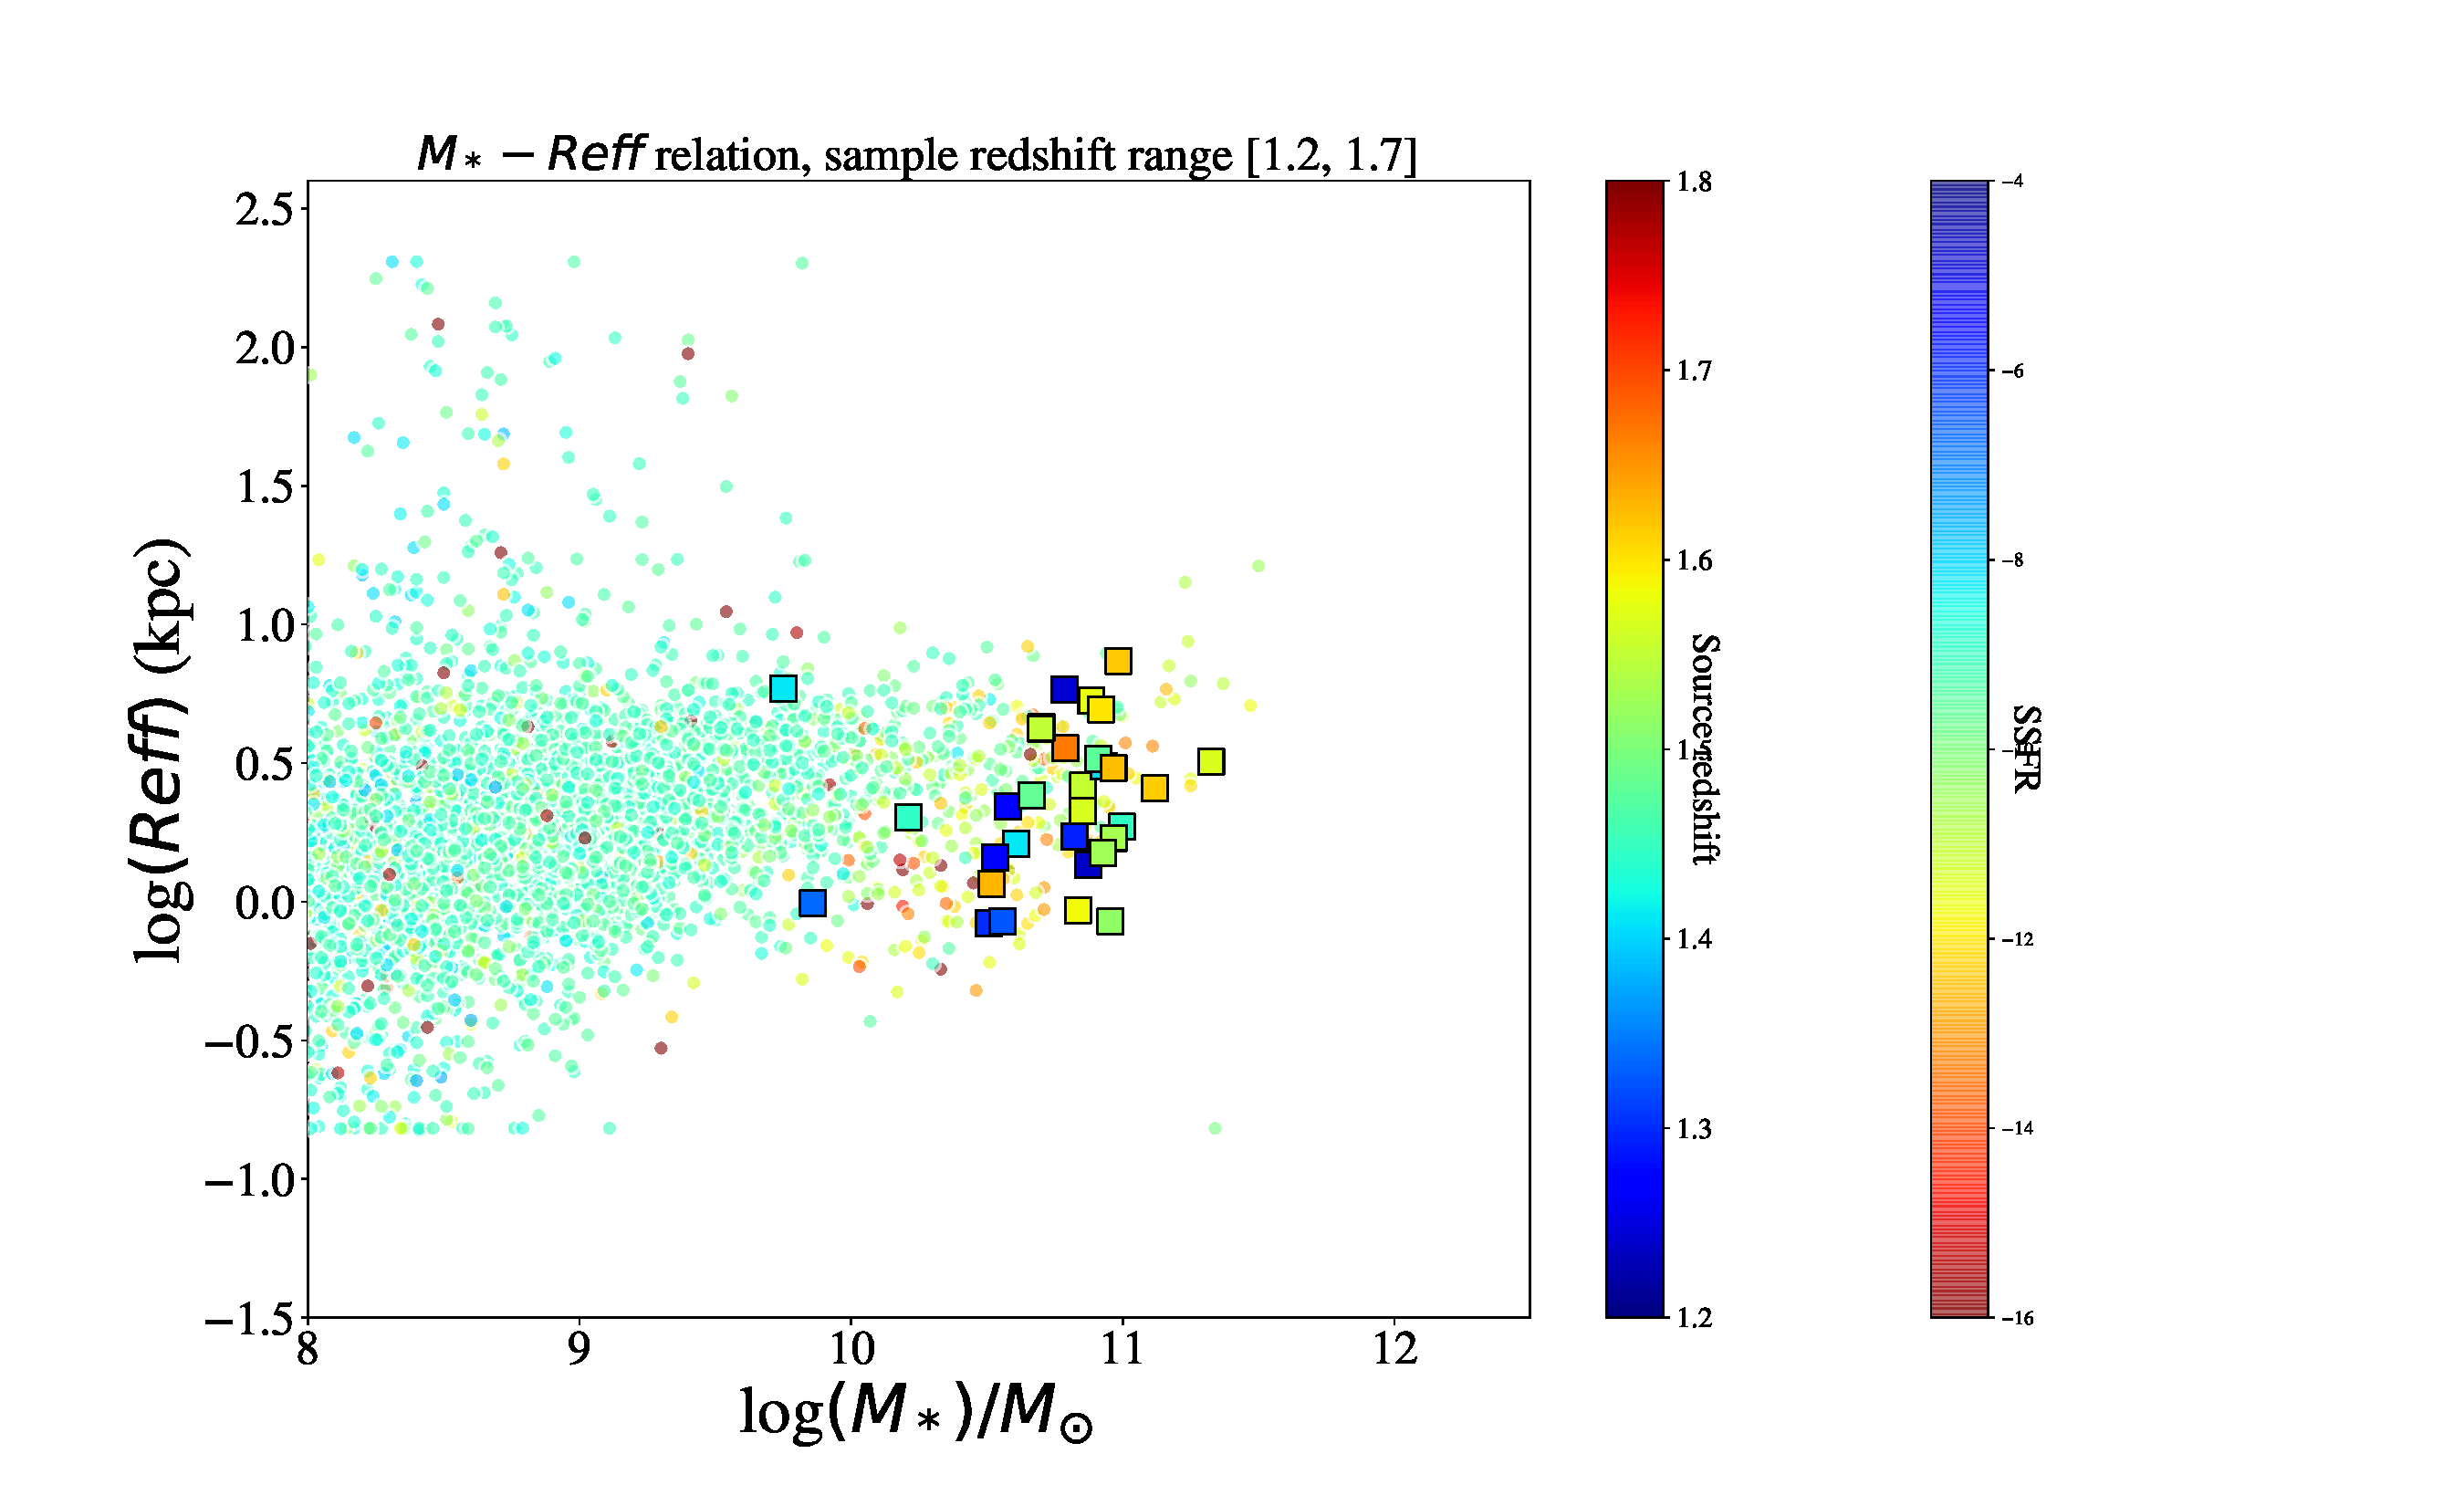
\includegraphics[trim = 0mm 0mm 90mm 0mm, clip, height=0.45\textwidth]{fig/Mstar-Reff.pdf}}&
{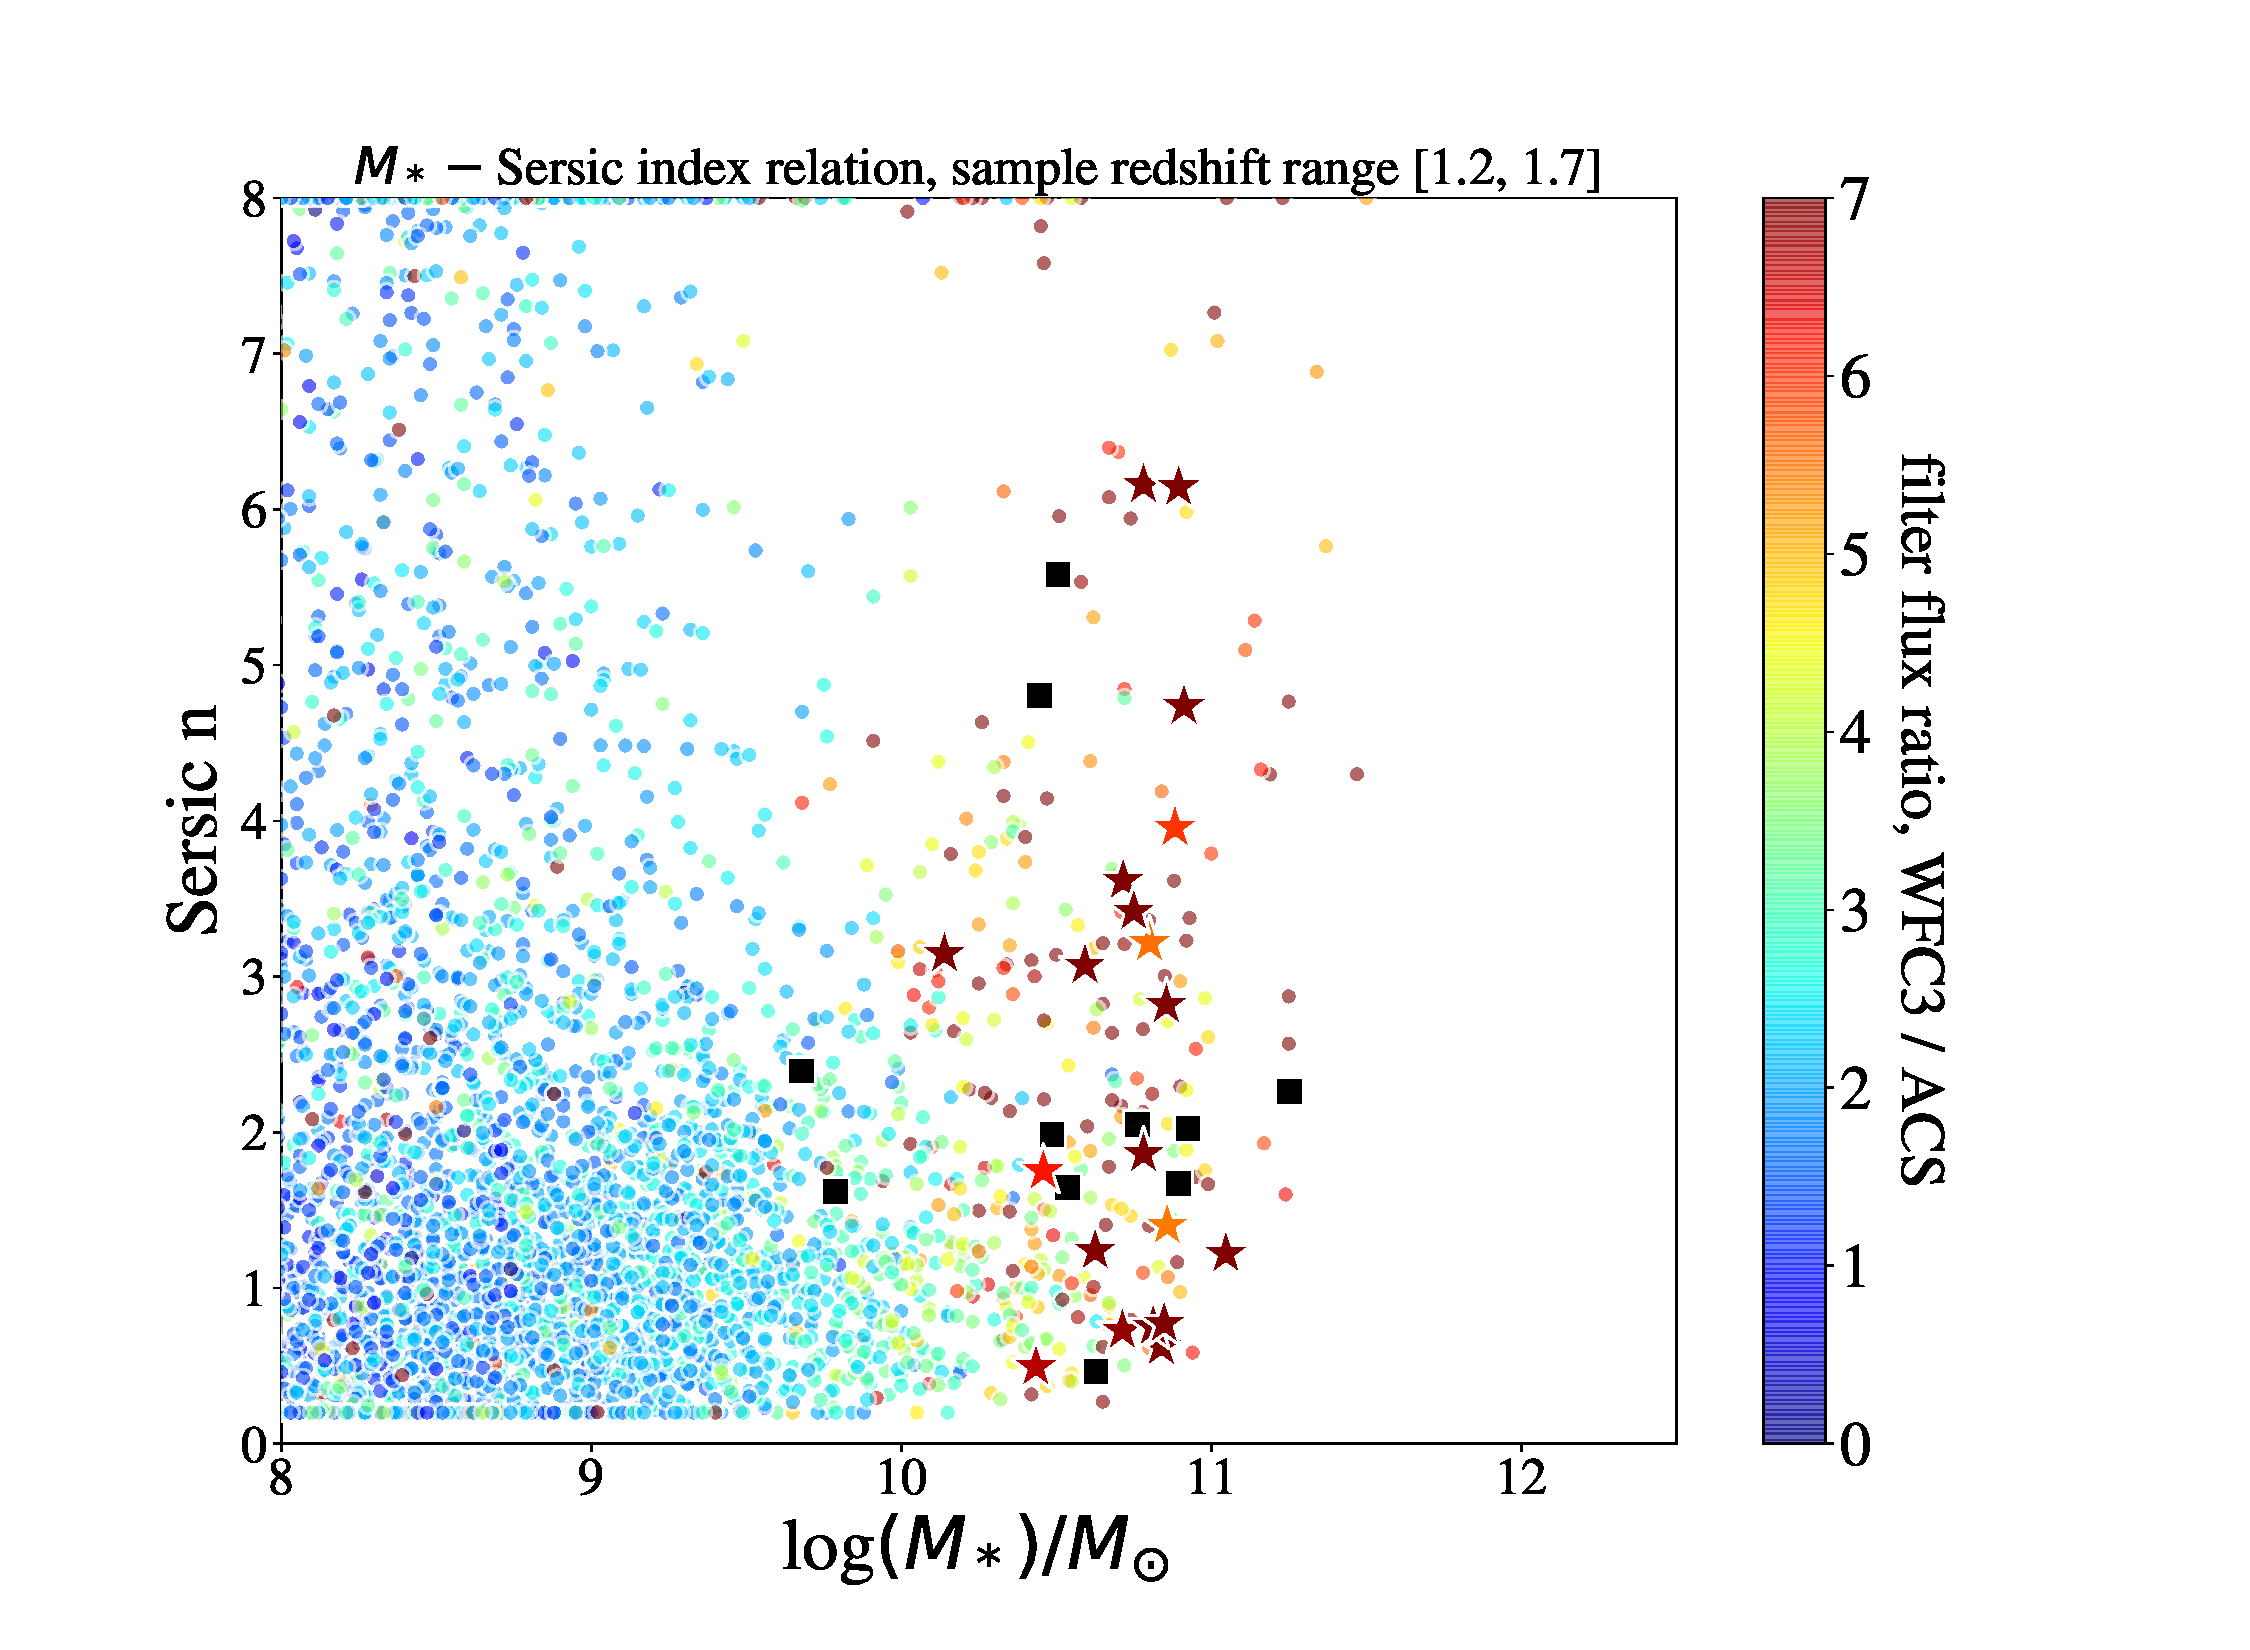
\includegraphics[ height=0.45\textwidth]{fig/Mstar-Sn.pdf}}\\
\end{tabular}
\caption{\label{fig:Mstar-rn} 
The comparison of the galaxy properties between our 32 AGNs' hosts to the CANDLES sample including 4401 inactive galaxies (circles). The color coding is based on the filter flux ratio between WFC3 and ACS. For CANDLES sample, the WFC3/F125W flux is taken. The black squares are the AGN samples with only WFC3 band observation.
}
\end{figure*} 

We also compare the histogram of the inferred \Reff\ and \sersic\ n to the inactive galaxies in Figure~\ref{fig:hist_rn}, where there is no significant difference between their distribution and median value. We perform the Kolmogorov-Smirnov test to interpret the p-value as 0.42 and 0.04 for \Reff\ and $n$, respectively. We thus conclude that the host galaxies of our AGN sample are representative of the overall population of galaxies at comparable luminosity and stellar mass at the same redshift.

\begin{figure}
\centering
{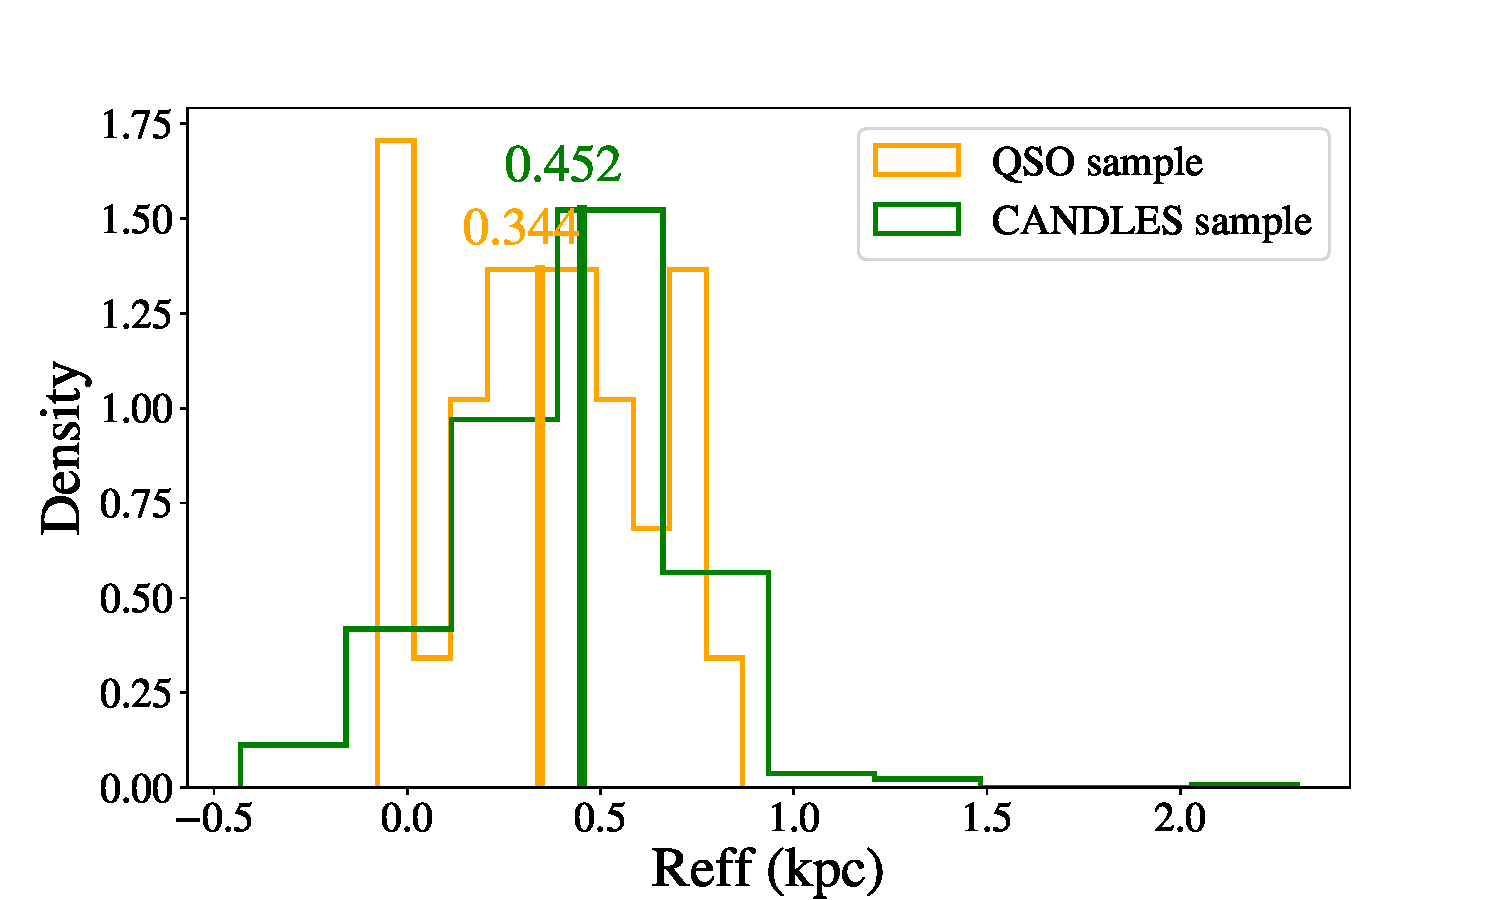
\includegraphics[ height=0.3\textwidth]{fig/Hist_Reff.pdf}}\\
{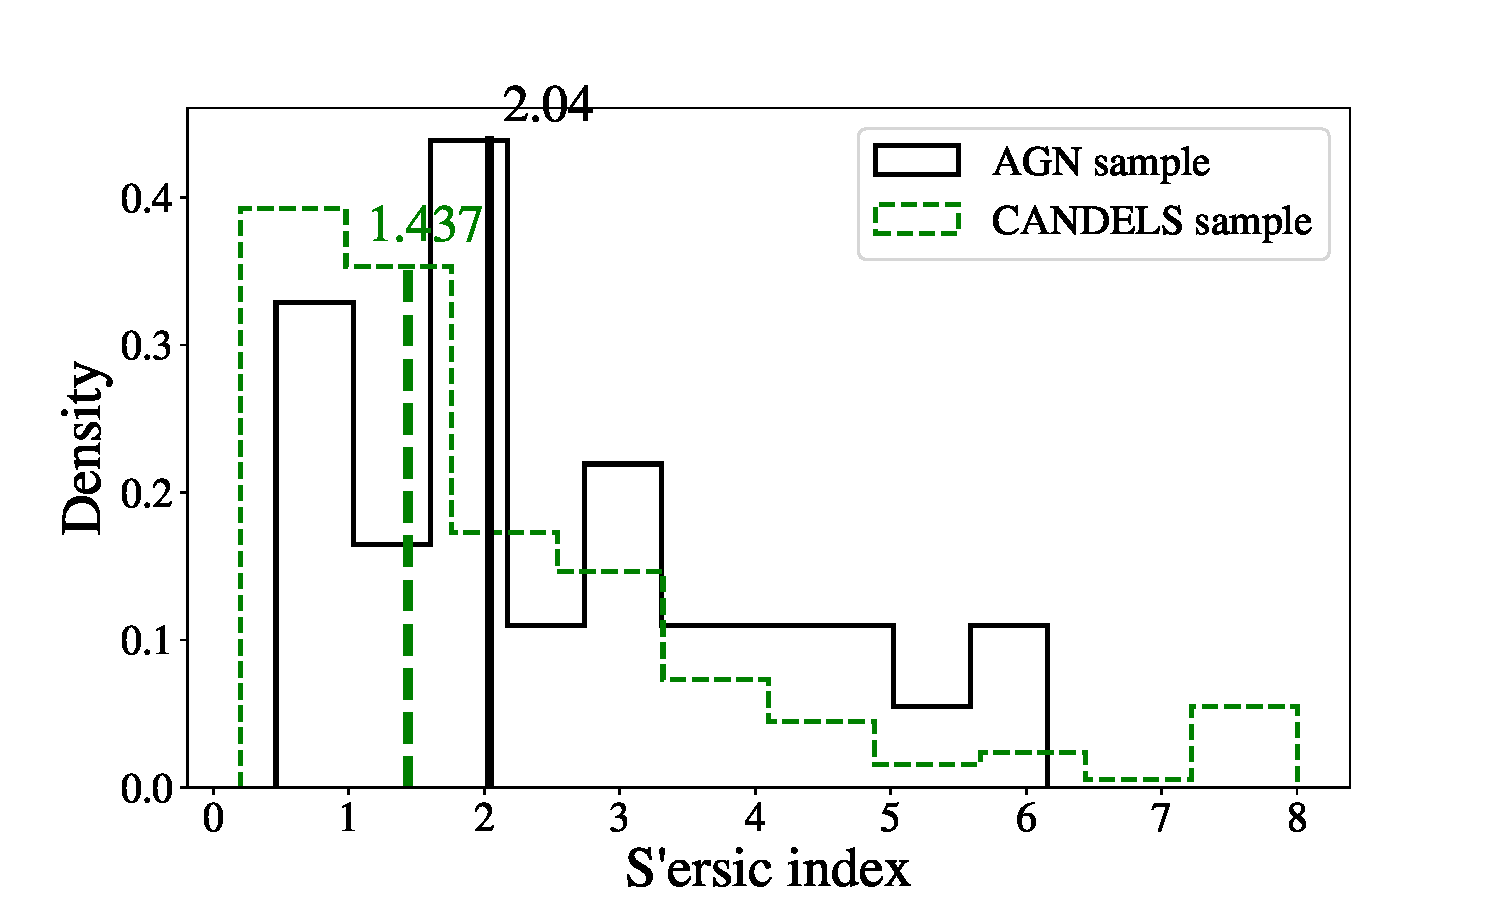
\includegraphics[ height=0.3\textwidth]{fig/Hist_Sn.pdf}}
\caption{\label{fig:hist_rn} 
The comparison of the histogram of the \Reff\ and \sersic\ n, with median value indicated.}
\end{figure} 

%The distribution shows that our AGN host are located at a higher end of the stellar mass at region where 

\subsection{JWST}
\textcolor{red}{Xuheng: some comments on JWST have been made at the end of the Summary. Do we need to put more discussion here?}

\section{Summary} \label{sec:sum}
We studied the evolution of the correlations between the supermassive black hole and their host galaxies using new measurements of 32 X-ray selected AGNs at $1.2<z<1.7$.

We used the published near-infrared spectroscopic observations \halpha\ and \hbeta\ emission lines to estimate the reliable values of BH mass. To obtain the properties of the AGN host galaxies, we performed the AGN image decomposition using the state-of-the-art techniques. We adopted the \hst/WFC3 infrared channel to observe the high-resolution AGN imaging data and collected the PSF-stars in across all the fields to build to a library of PSF for the fitting. Using the latest image modeling tool \lenstronomy, we decomposed the AGN image in 2-D plane taking each PSF in the library. We obtained the host \sersic\ property (i.e., host flux, effective radius, \sersic\ index) using a weighted arithmetic mean based on the inference by the eight top-ranked PSFs. Incorporating with the inference by \hst/ACS image, we selected the stellar population, hence derived the rest-frame R band Luminosity (\lhost) and stellar mass of the host (\smass).

Combining out high-$z$ measurements with the intermediate redshift samples from the literature~\citep{Park15, Bennert11, SS13}, we compared the scaling relations to the ones by the local with main results summarized as follows:
\begin{enumerate}
\item The \mbh-\smass\ relations at higher redshift are inconsistent with the local ones, i.e. Figure~\ref{fig:MM}, \ref{fig:MM-vz}.
\item Considering the correction for passive evolution of galaxy luminosity, the \mbh-\lhost\ relations at higher redshift are inconsistent with the local ones,  i.e. Figure~\ref{fig:ML-vz}.
\item The offsets of by the evolution are well described by the form $\Delta\log\mathcal M_{\rm BH}= \gamma \log (1 + z)$. Taking intro account selection effect, we obtain $\gamma = 0.8\pm0.3$ (\mbh-\smass) and $\gamma = 0.6\pm0.3$ (\mbh-\lhost).
\item We compare the properties of our active galaxy sample to the ones from inactive galaxy in the CANDLES imaging survey at the same redshift range, finding no significant discrepancy among them.
\end{enumerate}

Our inference indicates the evidence of disk component, i.e. the ones with \sersic\ $n<2$, and the local comparing samples are bulge dominated sample, we hence conclude that the BHs 8-10~Gyrs ago reside in bulges, if not entire galaxies, which are less massive/luminous than today.

Towards a better estimation of the evolution of the scaling relations, we need to address the limitations of this work. First, most of the host-total ration in the \hst/ACS band, the fidelity of the host flux are thus limited at UV. We thus adopt a universal stellar template to the overall galaxies based on the general inference between UV band and IR band, rather than carry out the SED fitting for each galaxy, to derive the \lhost\ and \smass. Second, at this moment, the local scaling relations that we current have are not yet solid. We have found the values of $\gamma$ could vary from 0.8 to 2.0, using different local sample from different literature \citep{Ben++10, Bennert++2011, H+R04, Kormendy13, Bentz2018}. Thus, a solid sample served as the local anchor still needed to be well defined (Bennert et al., in prep). One the other hand, comparing the observational measurements to the ones by the simulation could avoid not only the dependency to the local anchor, but also the bias by selection effect \citep{DeG++15, Khandai2015, Menci2014}. To overcome these limitation, we are currently incorporating our measurement with the ground-based photometry to derive SED fitting, in order to compare with the sample by simulations, which will be presented in our coming up paper.

Looking into the future, the forthcoming lunching of {\it James Webb Space Telescope} ({\it JWST}) would provide the high quality imaging data of AGN at higher redshift (up to $z\sim$7-10) and thus trace the evolution of correlation at more distant universe. Furthermore, {\it JWST} is capable of showing the morphology of structures feeding black hole accretion and feedback on the host galaxy~\citep{Ford2014}, thus providing the opportunity to understand the origin of the scaling relations and their evolution.
}


\section*{Acknowledgments}
Based in part on observations made with the NASA/ESA Hubble Space Telescope, obtained at the Space Telescope Science Institute, which is operated by the Association of Universities for Research in Astronomy, Inc., under NASA contract NAS 5-26555. These observations are associated with programs
\#15115. Support for this work was provided by NASA through grant number HST-GO-15115 from the Space Telescope Science Institute, which is operated by AURA, Inc., under NASA contract NAS 5-26555.

The authors fully appreciate the discussions with Hyewon Suh, Vardha N. Bennert, Anton M. Koekemoer, Takahiro Morishita.

XD, SB and TT acknowledge support by the Packard Foundation through a Packard Research fellowship to TT.

This work has made use of \lenstronomy~\citep{lenstronomy}, {\sc Astropy}~\citep{Astropy}, {\sc photutils}~\citep{photutils}, {\sc TOPCAT}~\citep{TOPCAT}, {\sc Matplotlib}~\citep{Matplotlib} %, {\sc adjustText}~\citep{adjustText}
and standard Python libraries.

\bibliographystyle{apj.bst}
\bibliography{references}

\newpage
\appendix
\section{A. The demonstration of remaining 31 AGNs}\label{appA}
The AGNs decomposition for the other 31 objects of our sample, presented in the same way as Figure~\ref{fig:AGN_decomp}.

\begin{figure}[H]
\centering
%\hspace{-5.5em}
{
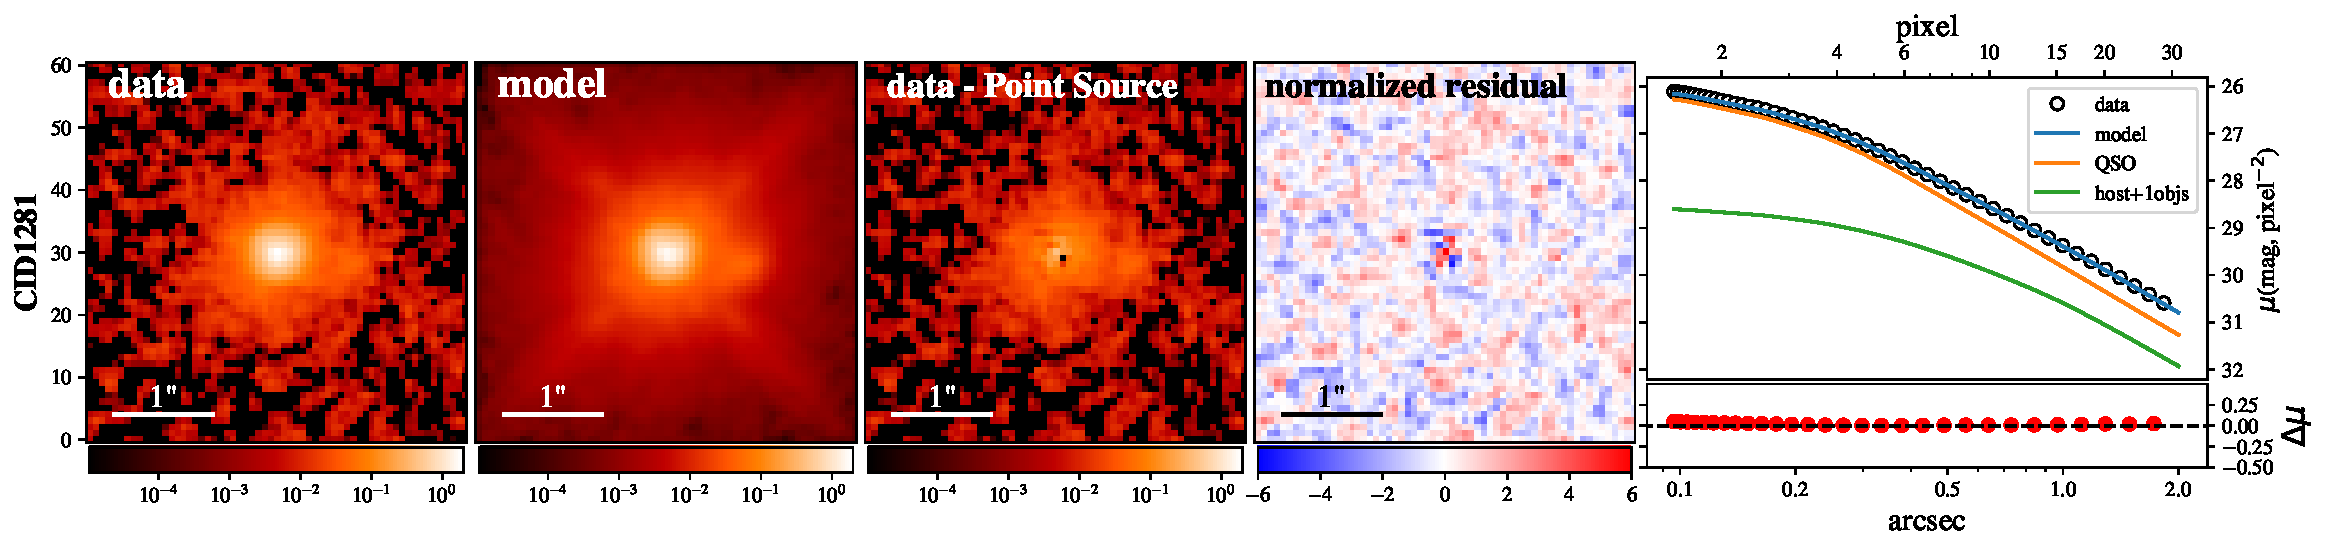
\includegraphics[height=0.25\textwidth]{fig/best_fit_CID1281_SB_profile.pdf}
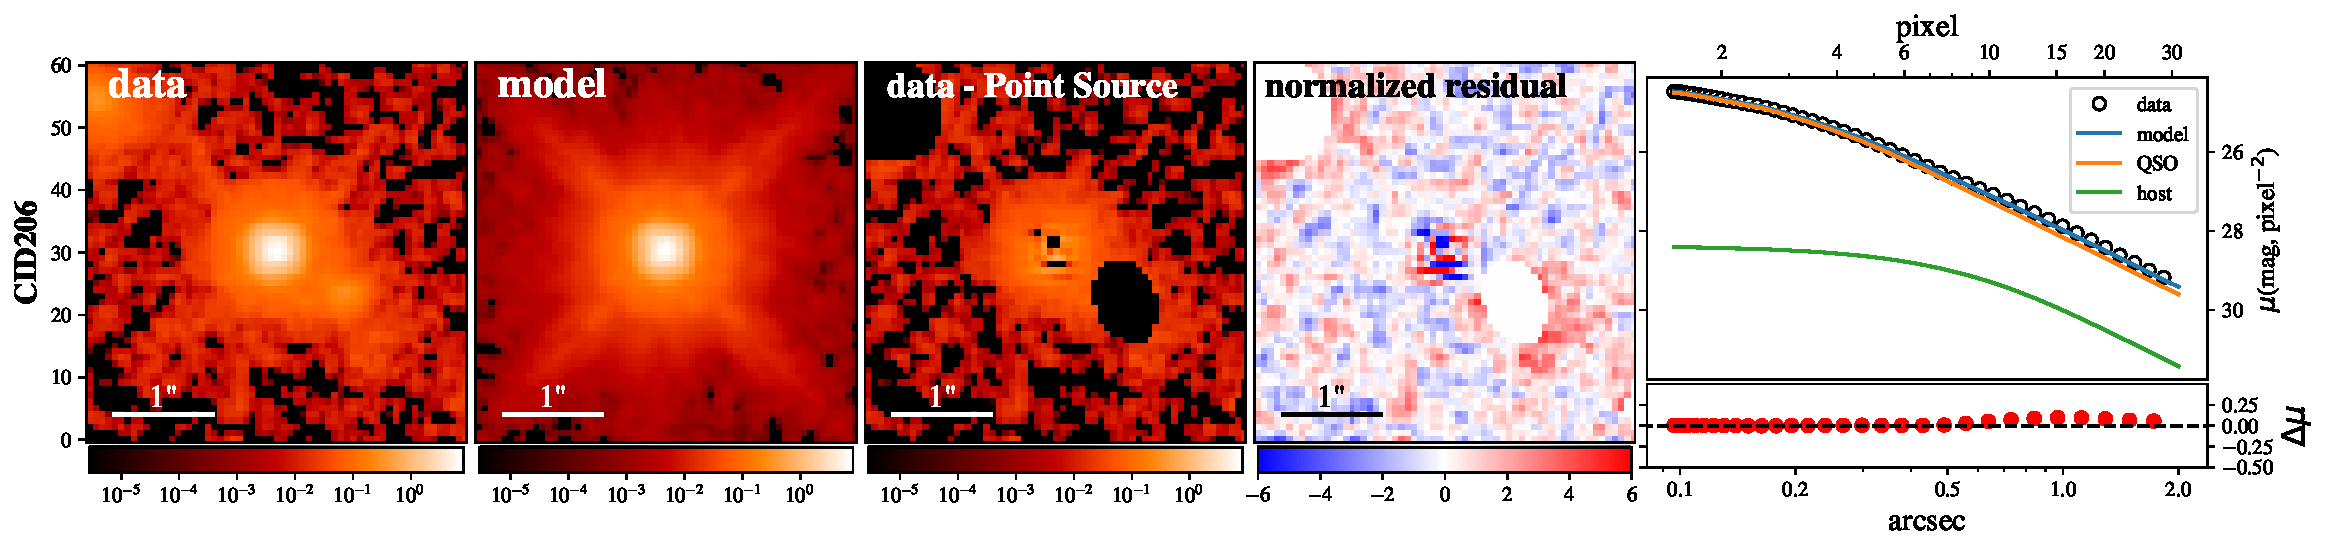
\includegraphics[height=0.25\textwidth]{fig/best_fit_CID206_SB_profile.pdf}
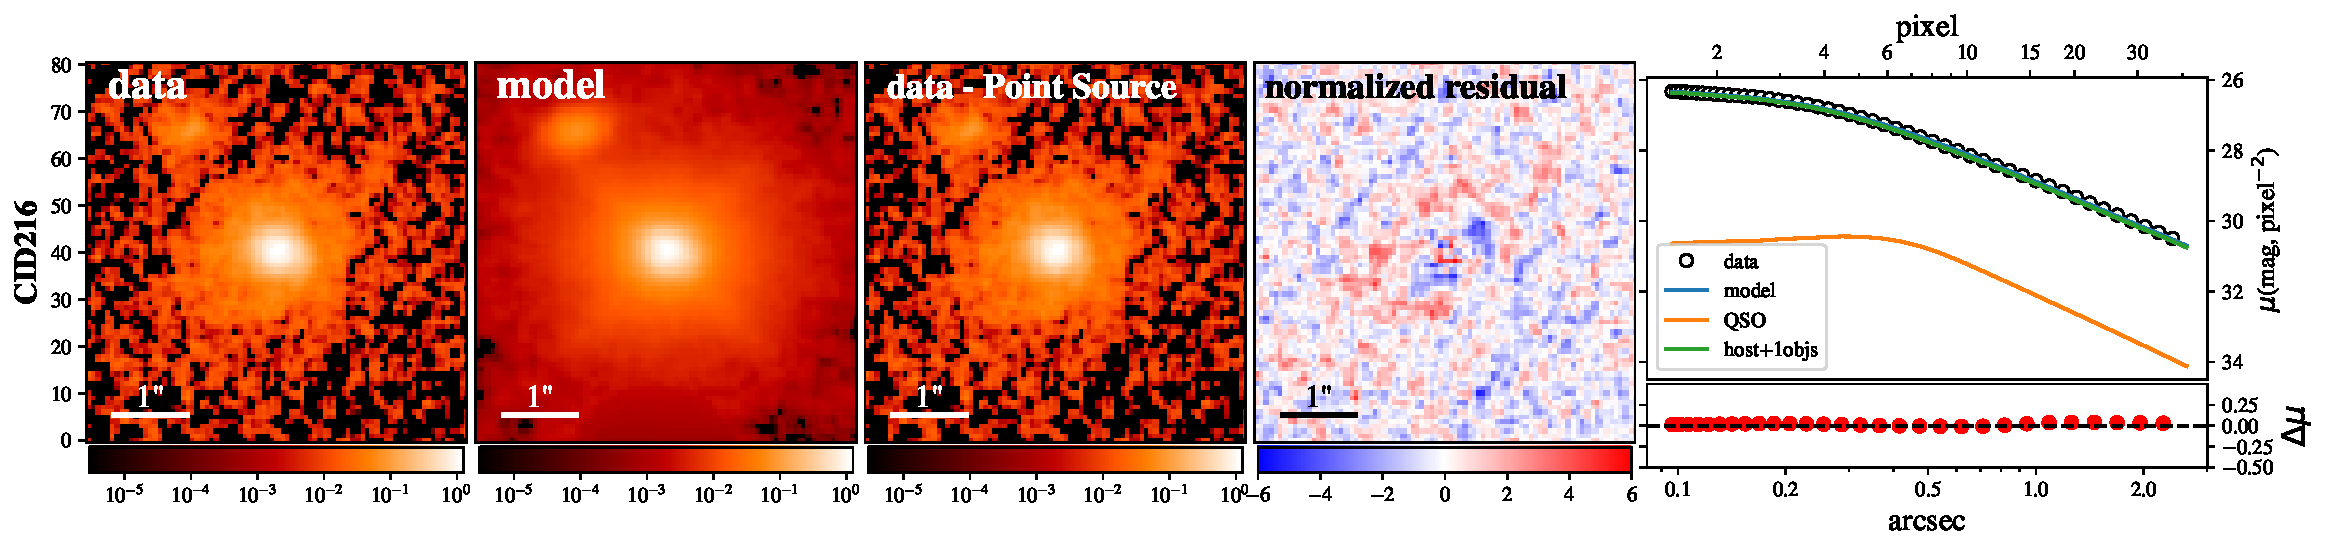
\includegraphics[height=0.25\textwidth]{fig/best_fit_CID216_SB_profile.pdf}
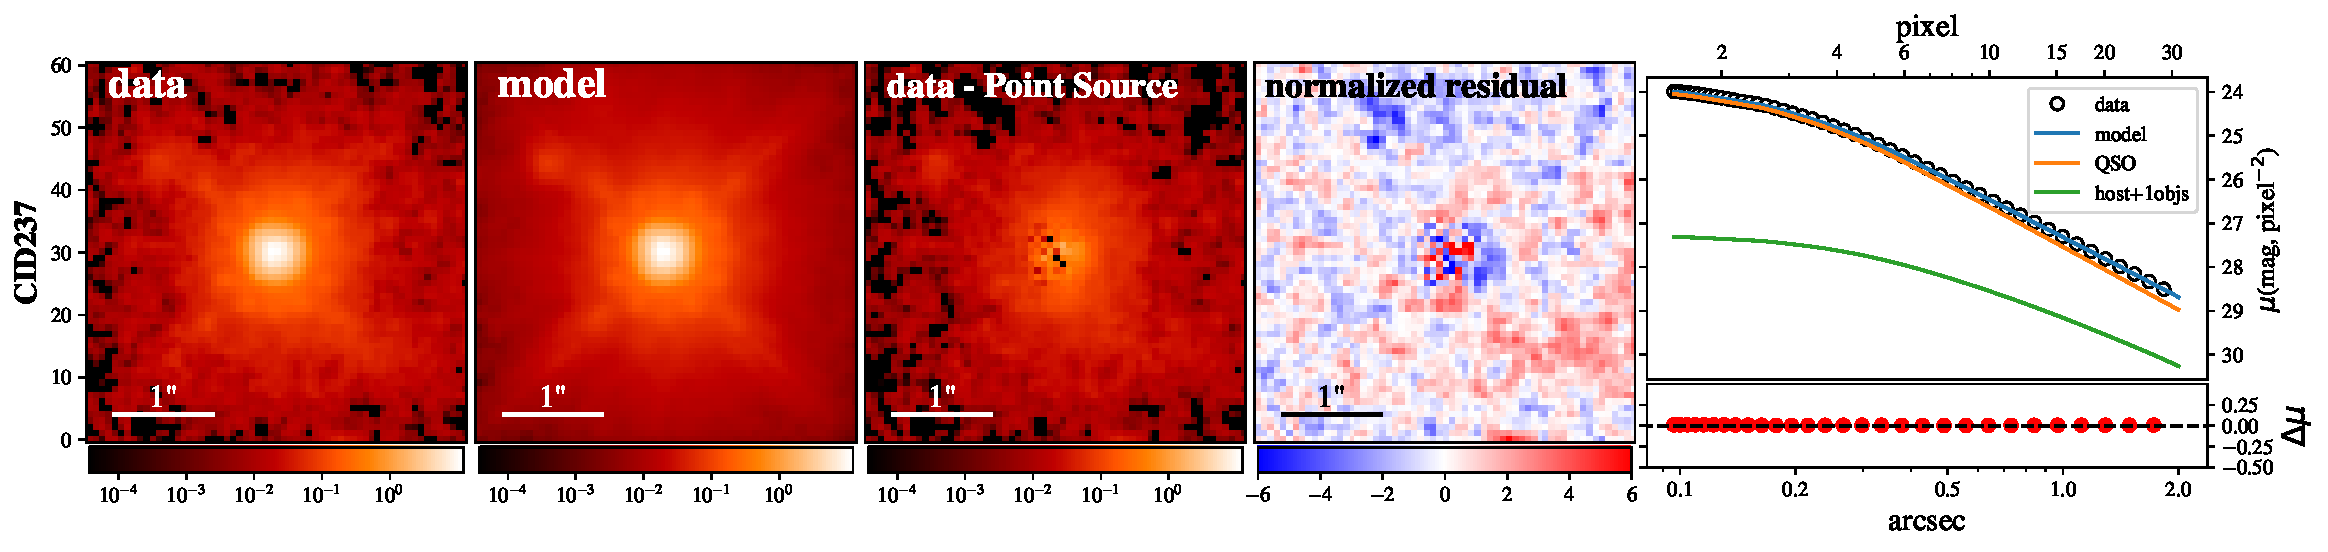
\includegraphics[height=0.25\textwidth]{fig/best_fit_CID237_SB_profile.pdf}
}
\end{figure} 

\begin{figure}
\centering
%\hspace{-5.5em}
{
\includegraphics[height=0.25\textwidth]{fig/best_fit_CID255_SB_profile.pdf}
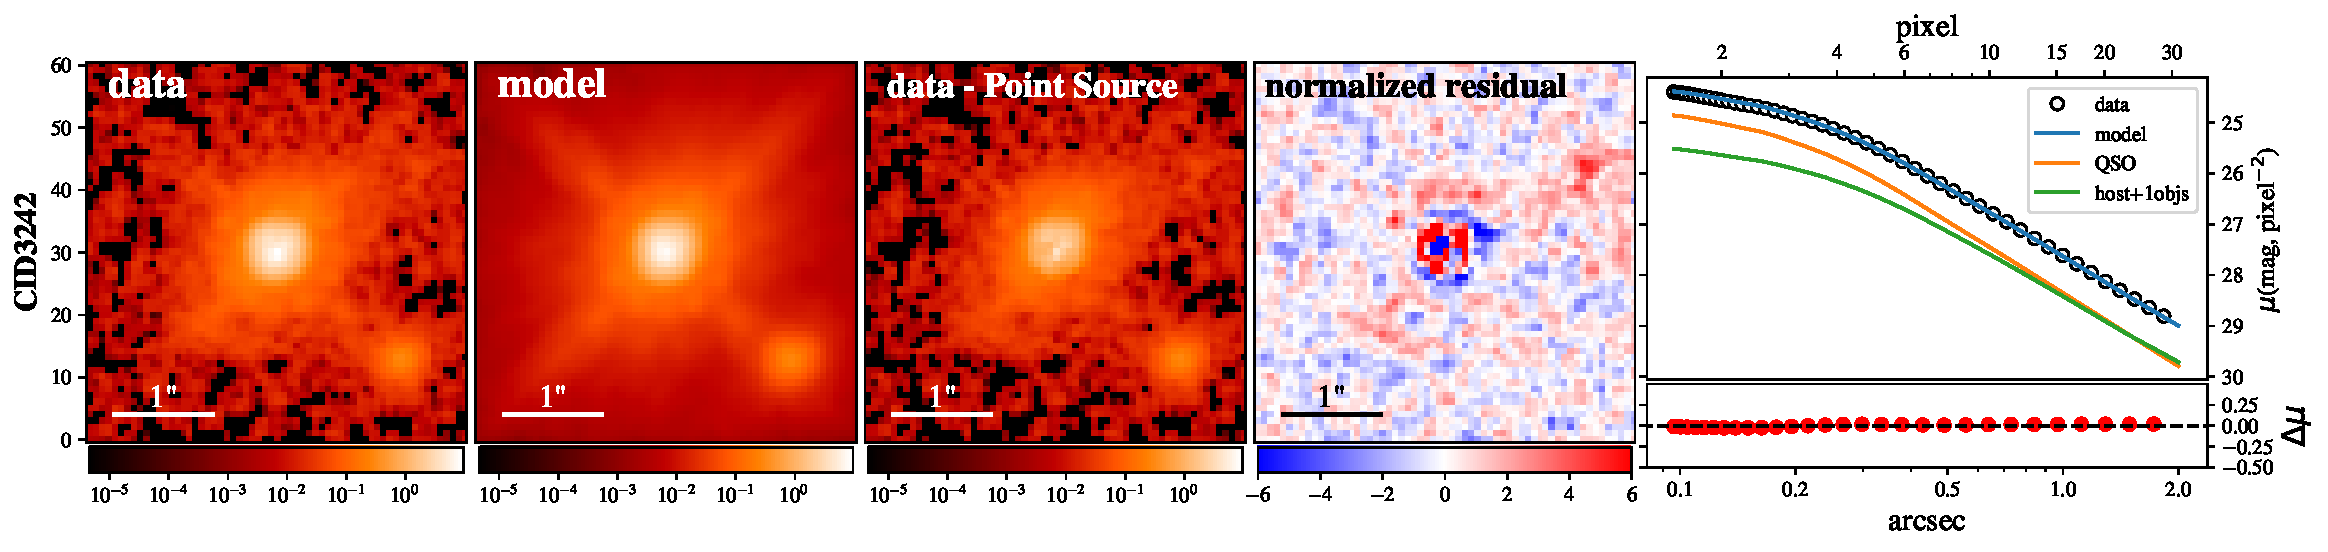
\includegraphics[height=0.25\textwidth]{fig/best_fit_CID3242_SB_profile.pdf}
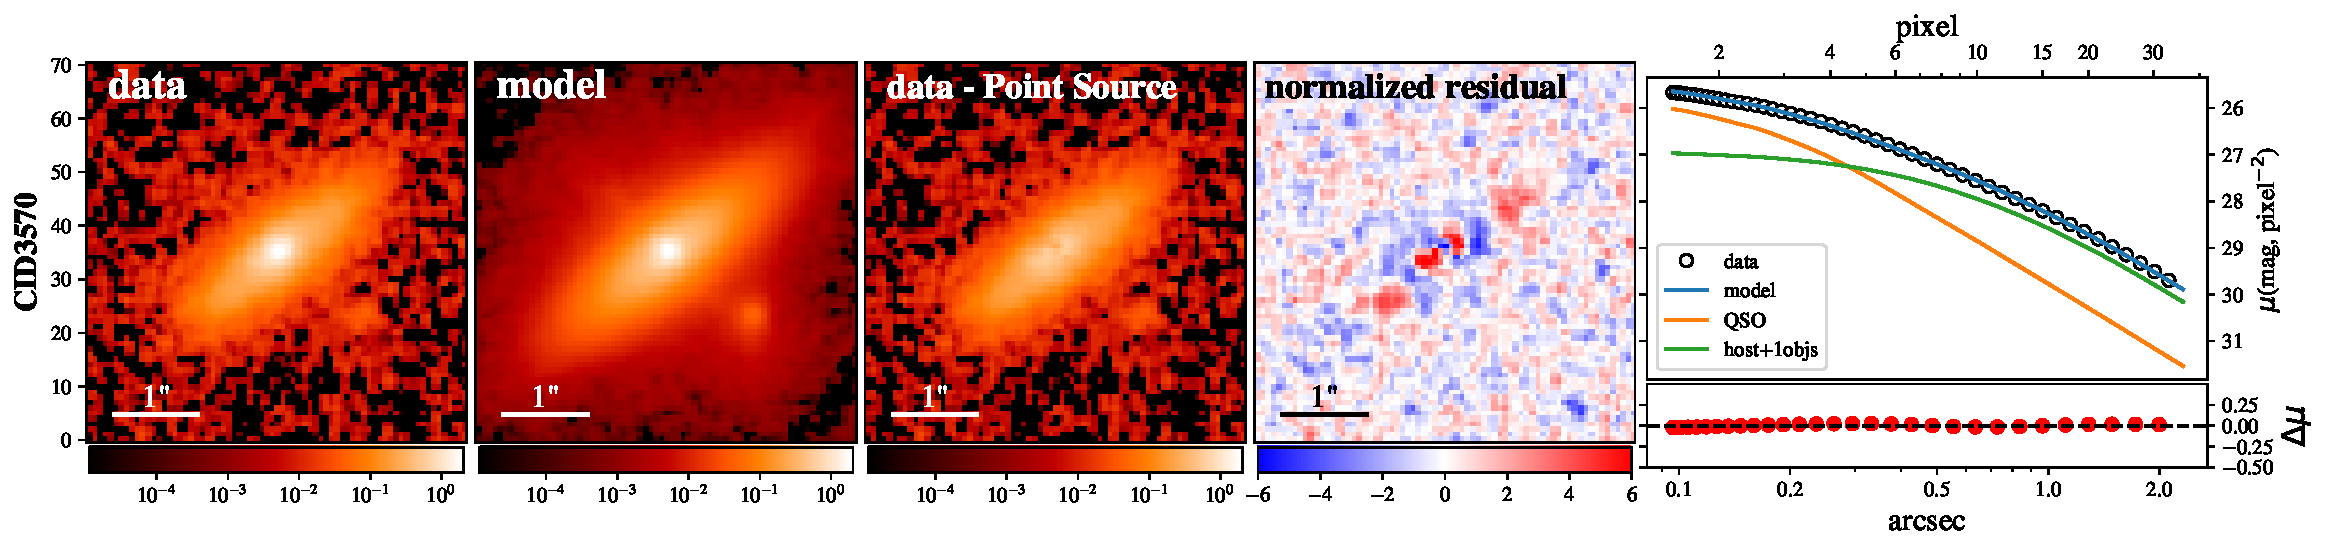
\includegraphics[height=0.25\textwidth]{fig/best_fit_CID3570_SB_profile.pdf}
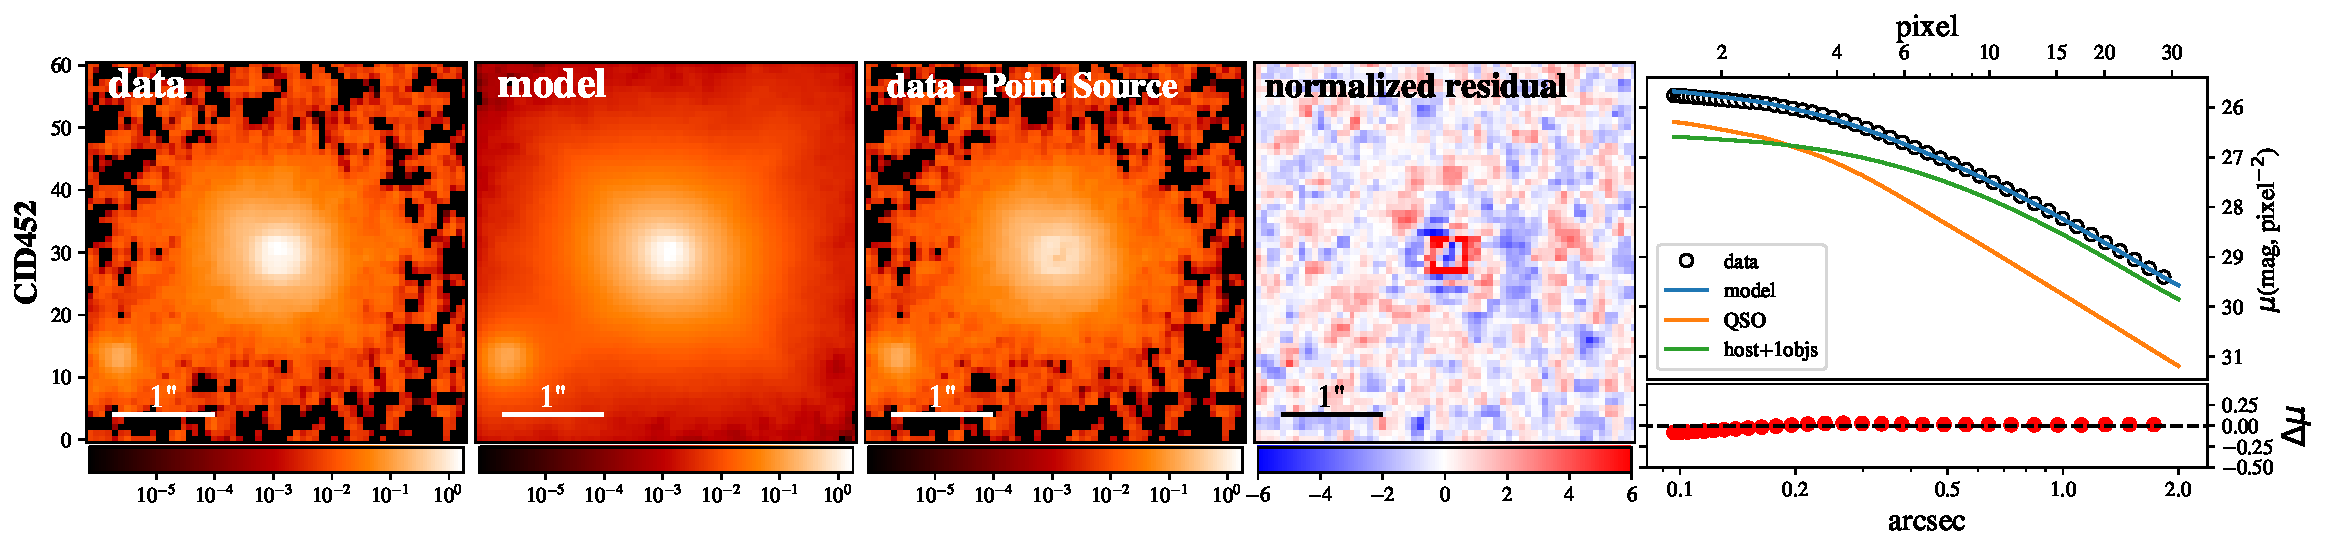
\includegraphics[height=0.25\textwidth]{fig/best_fit_CID452_SB_profile.pdf}
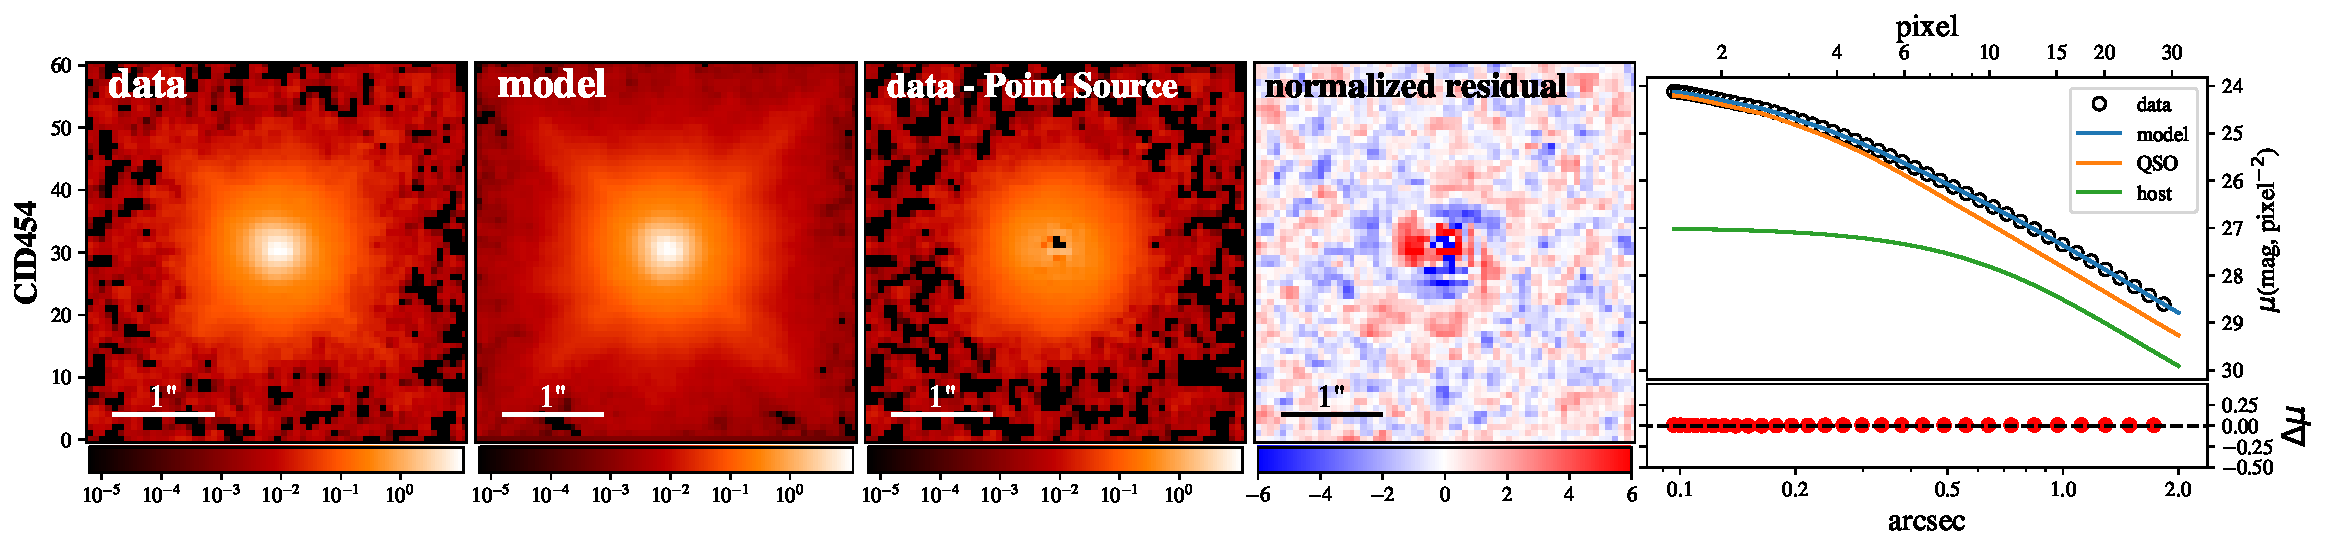
\includegraphics[height=0.25\textwidth]{fig/best_fit_CID454_SB_profile.pdf}
}
%\figurenum{1}
%\caption{Continued.}
\end{figure} 

\begin{figure*}
\centering
%\hspace{-5.5em}
{
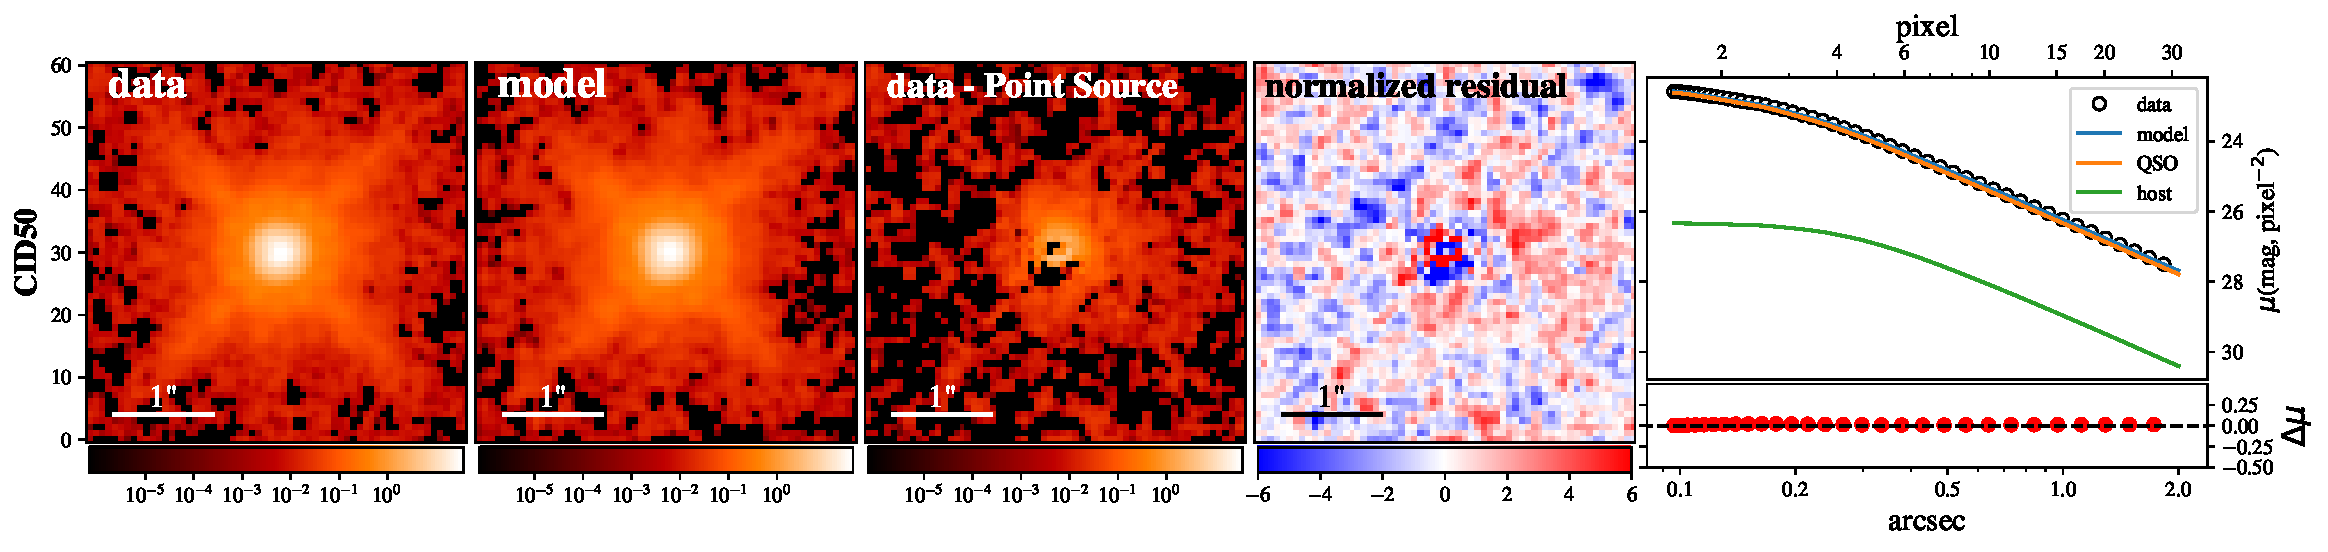
\includegraphics[height=0.25\textwidth]{fig/best_fit_CID50_SB_profile.pdf}
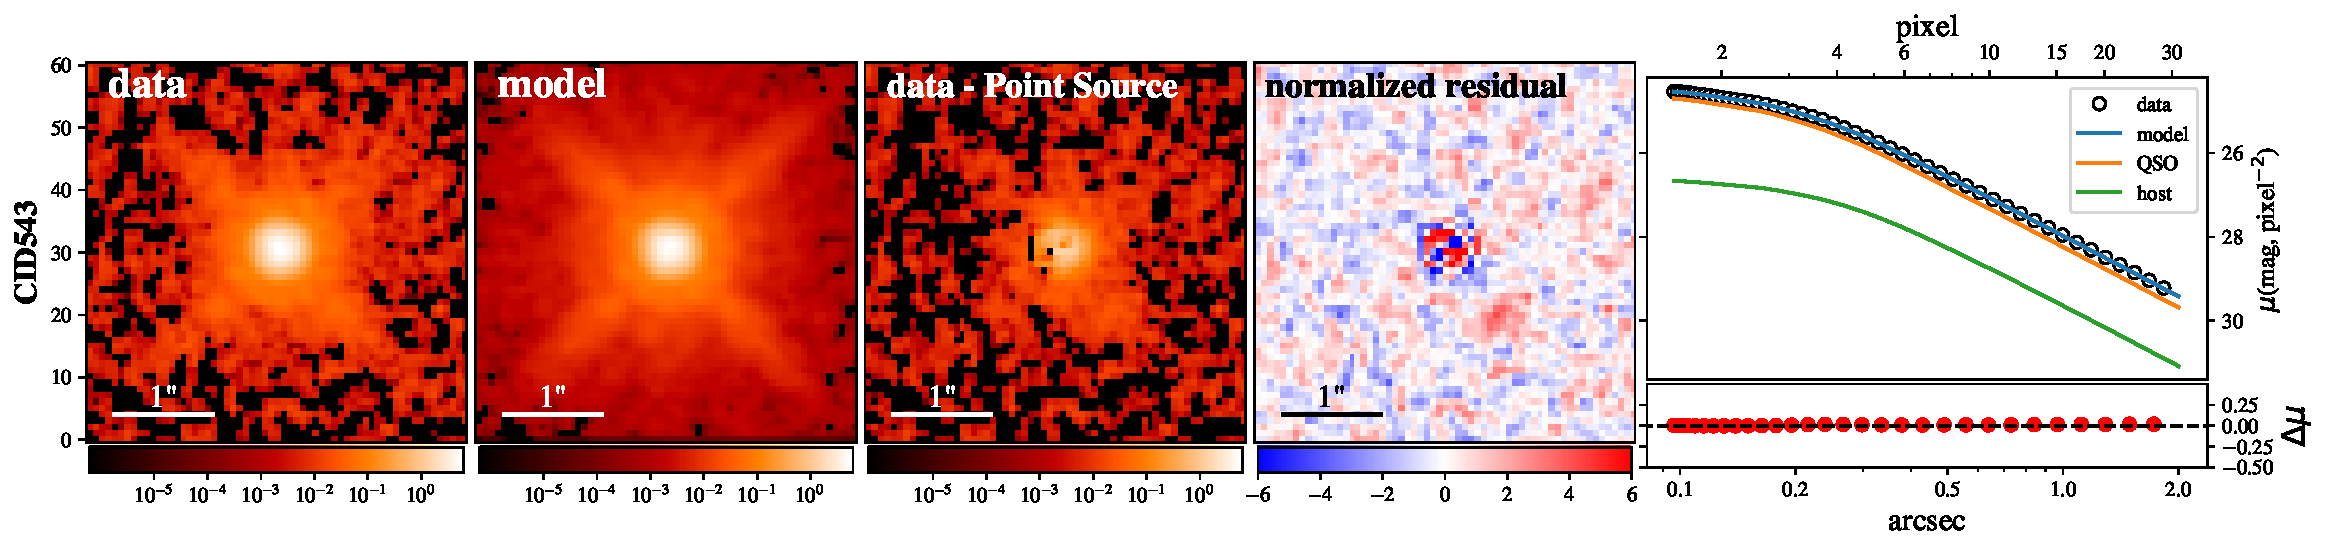
\includegraphics[height=0.25\textwidth]{fig/best_fit_CID543_SB_profile.pdf}
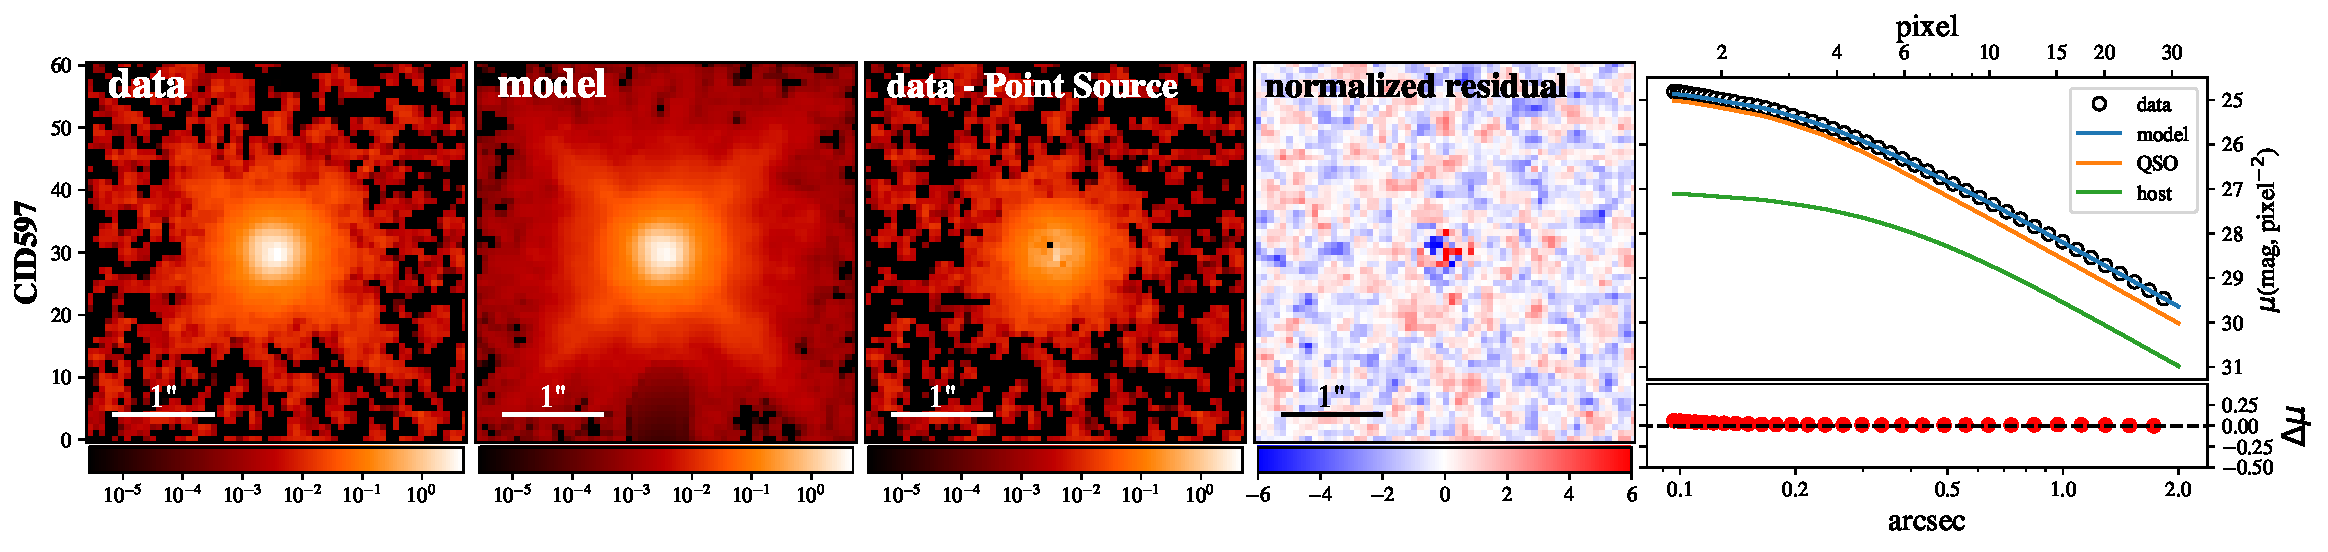
\includegraphics[height=0.25\textwidth]{fig/best_fit_CID597_SB_profile.pdf}
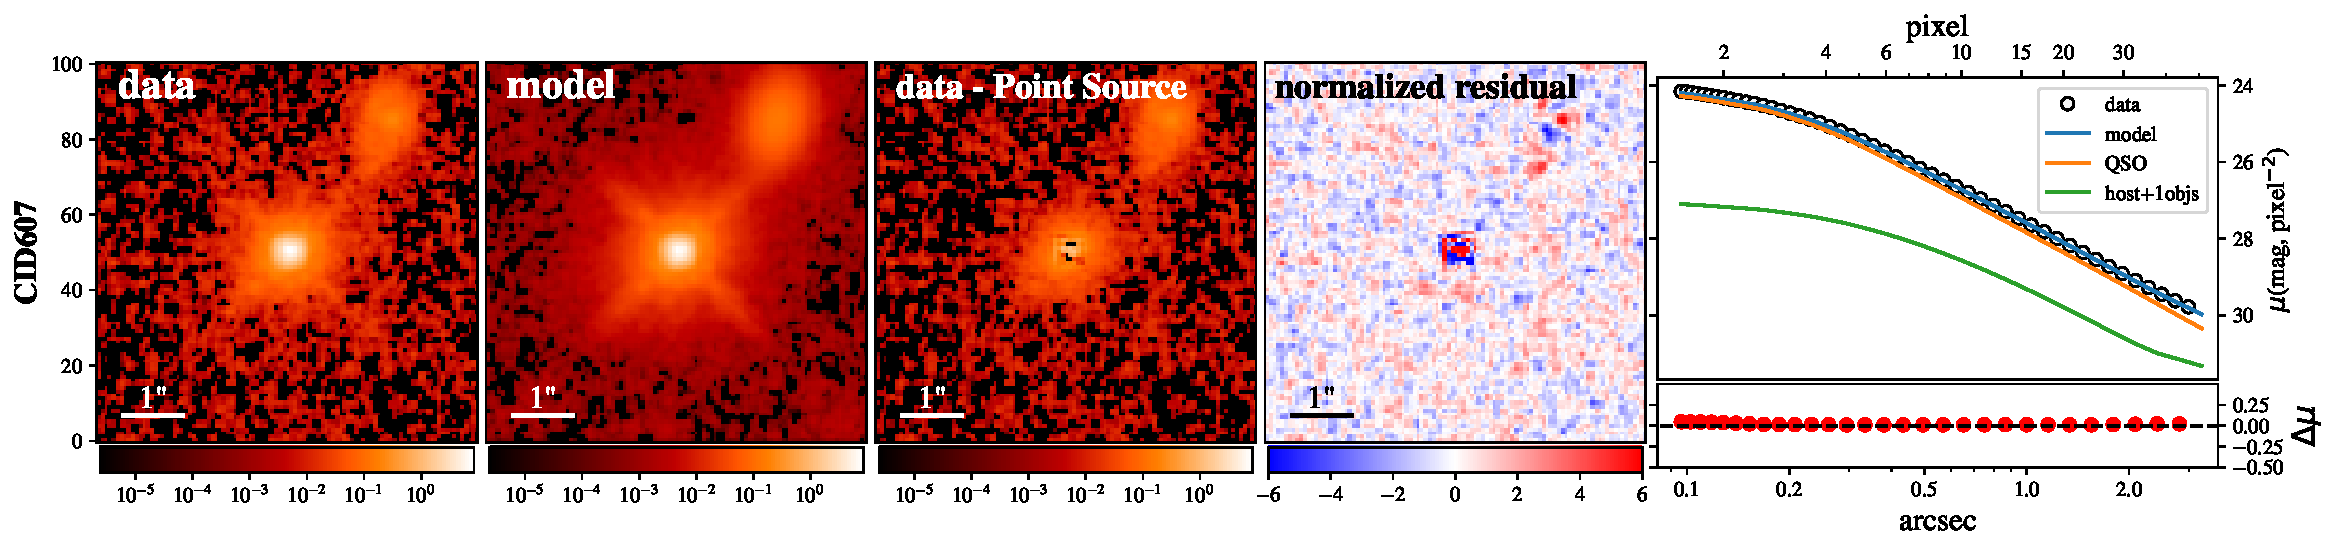
\includegraphics[height=0.25\textwidth]{fig/best_fit_CID607_SB_profile.pdf}
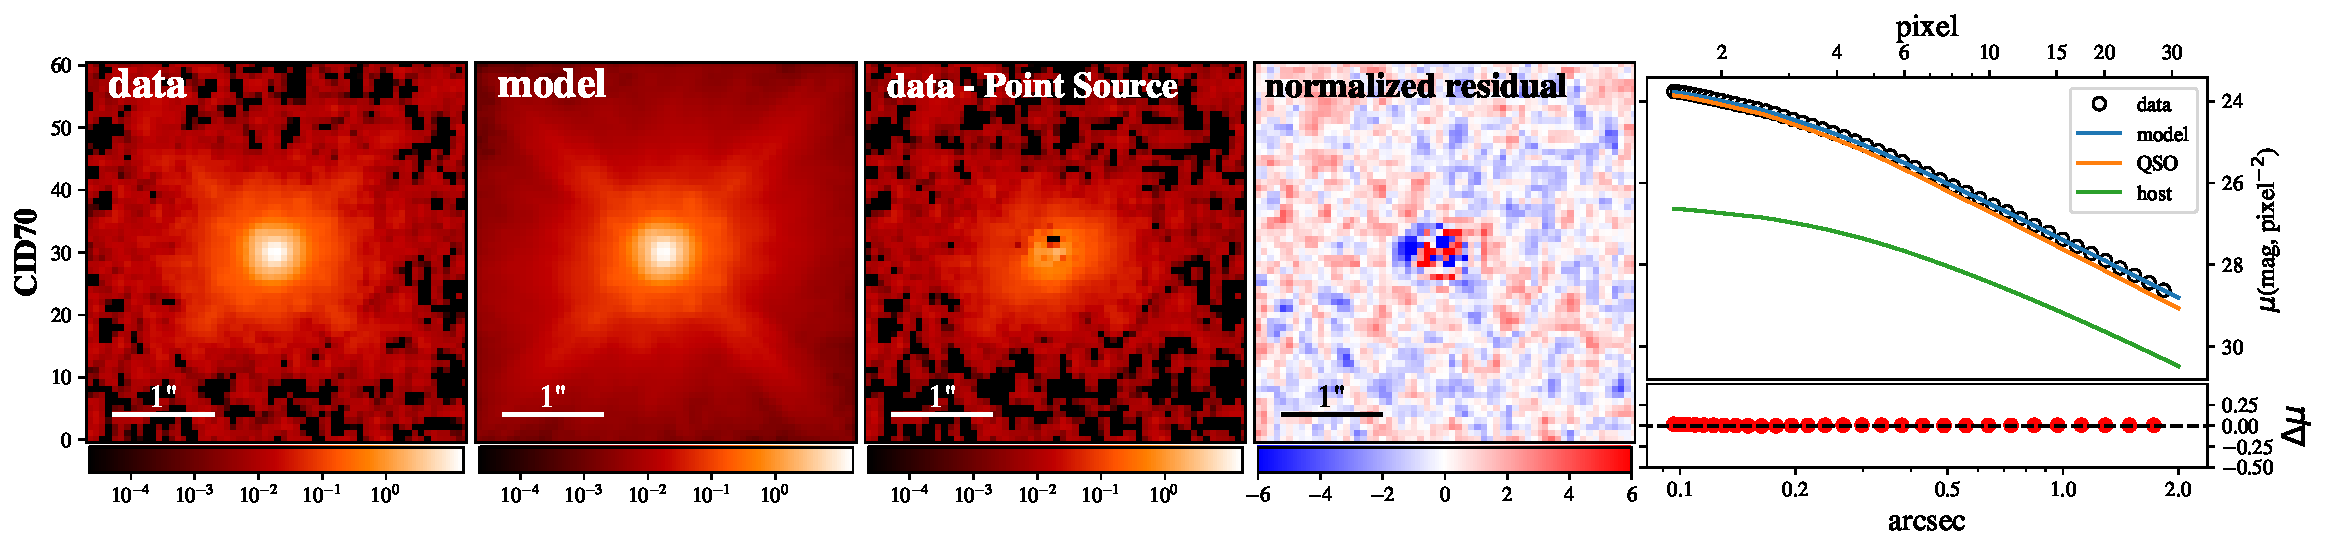
\includegraphics[height=0.25\textwidth]{fig/best_fit_CID70_SB_profile.pdf}
}
%\figurenum{1}
%\caption{Continued.}
\end{figure*} 

\begin{figure*}
\centering
%\hspace{-5.5em}
{
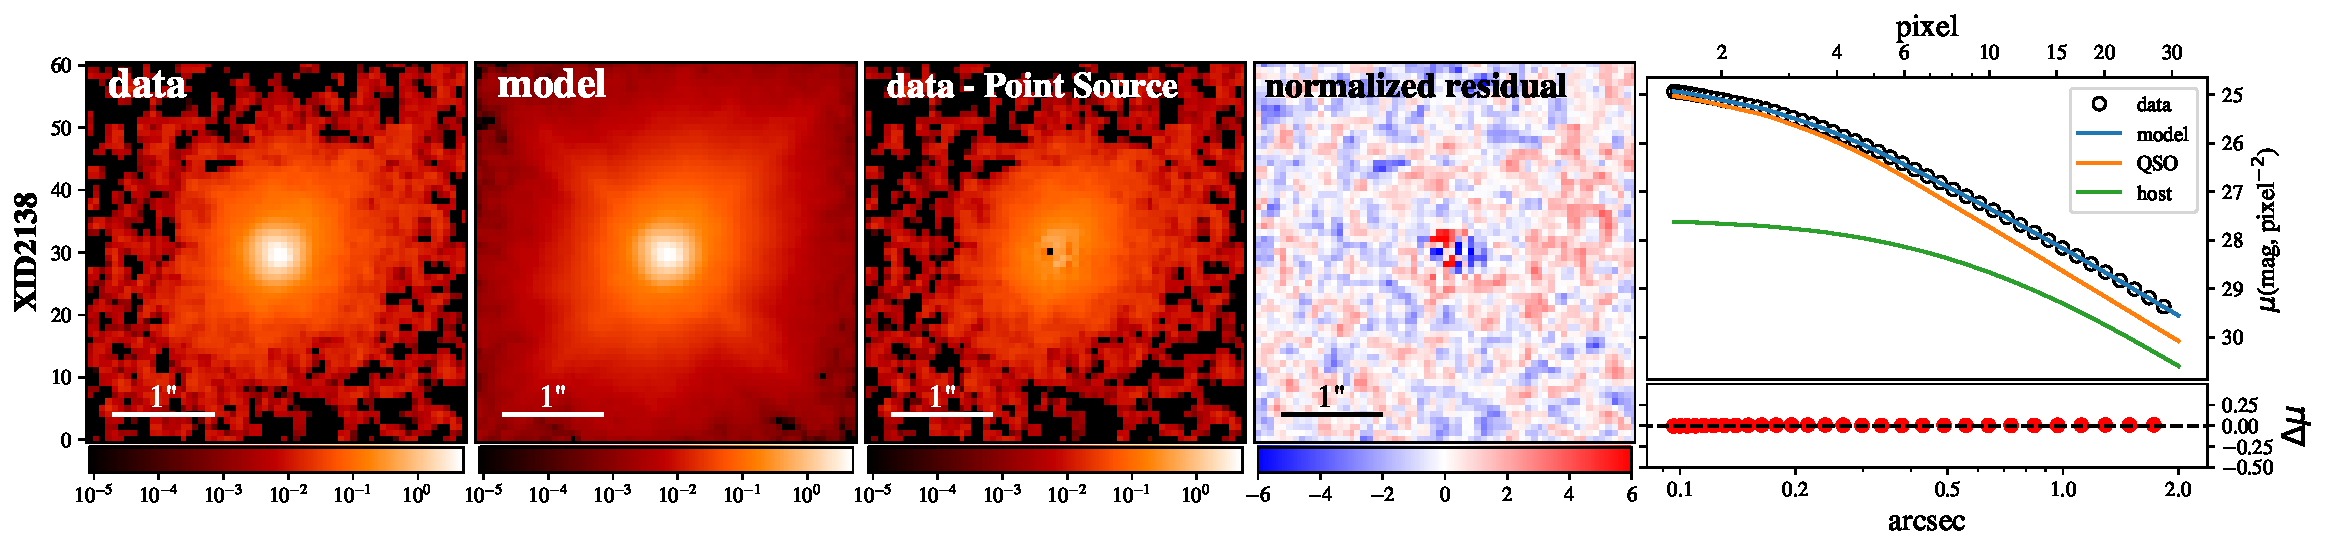
\includegraphics[height=0.25\textwidth]{fig/best_fit_XID2138_SB_profile.pdf}
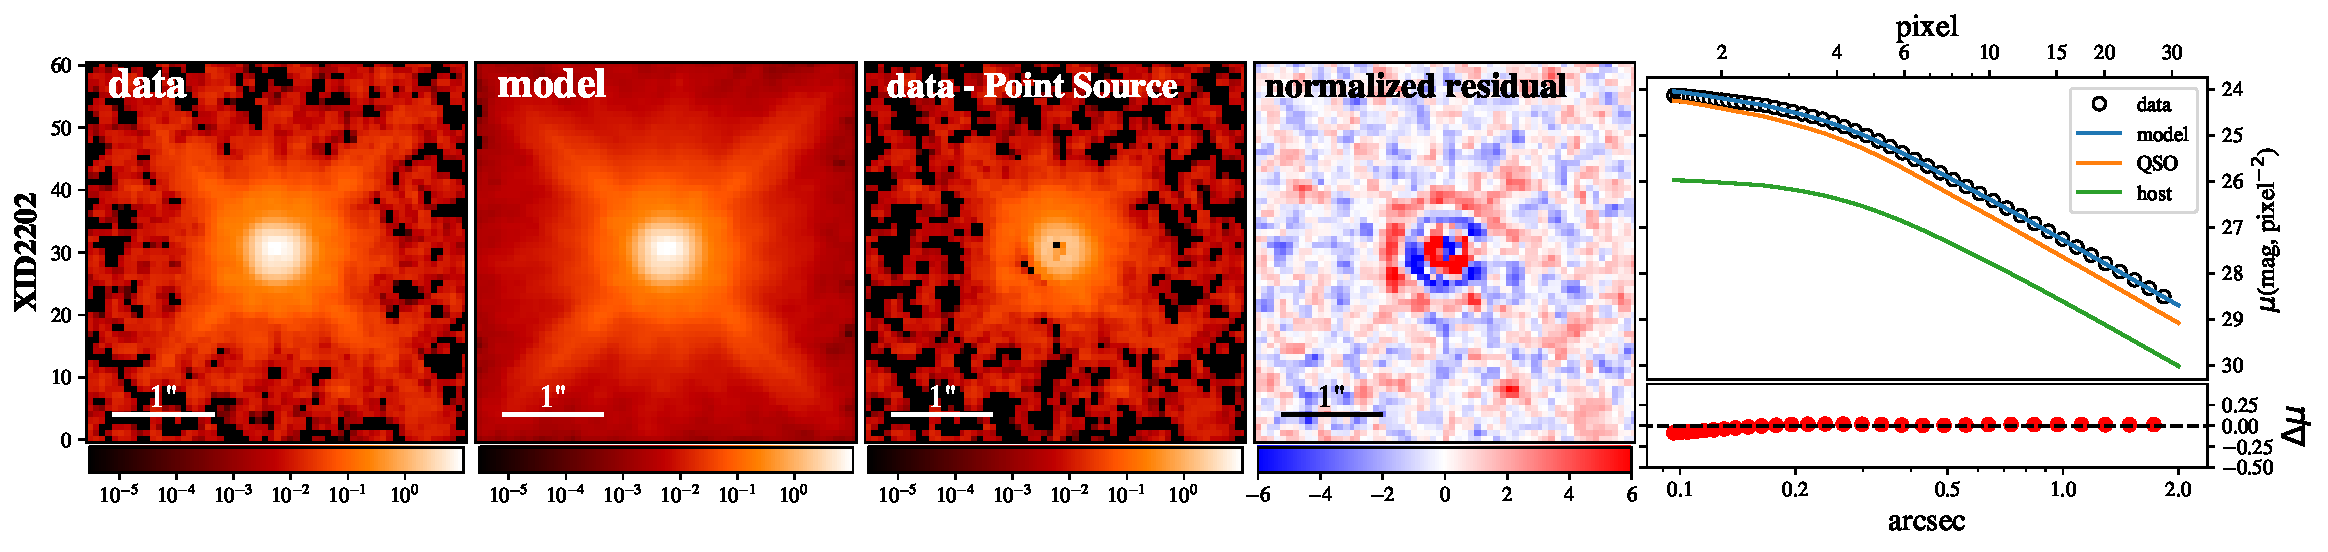
\includegraphics[height=0.25\textwidth]{fig/best_fit_XID2202_SB_profile.pdf}
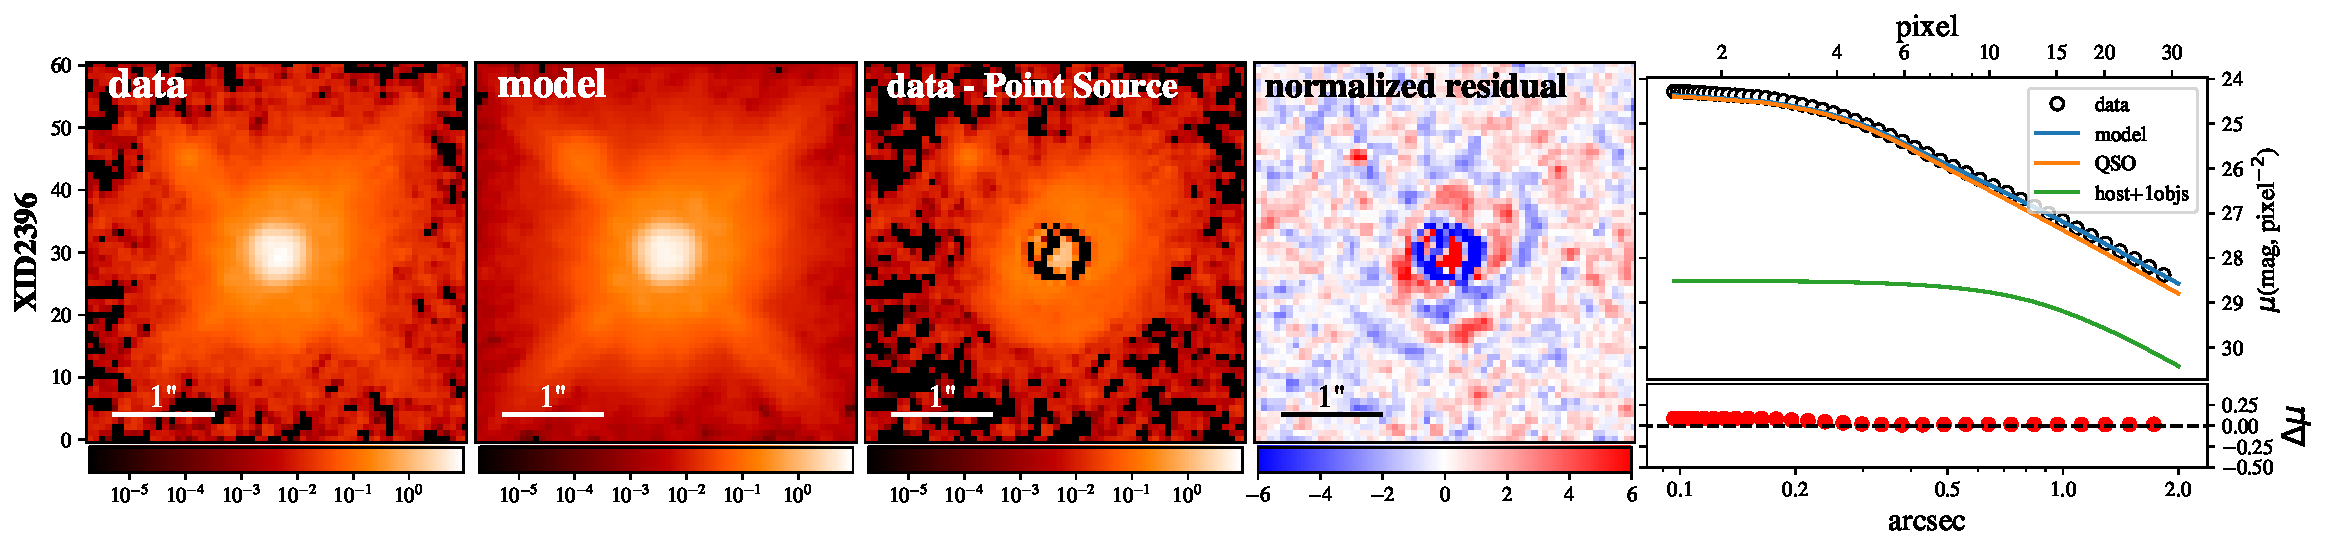
\includegraphics[height=0.25\textwidth]{fig/best_fit_XID2396_SB_profile.pdf}
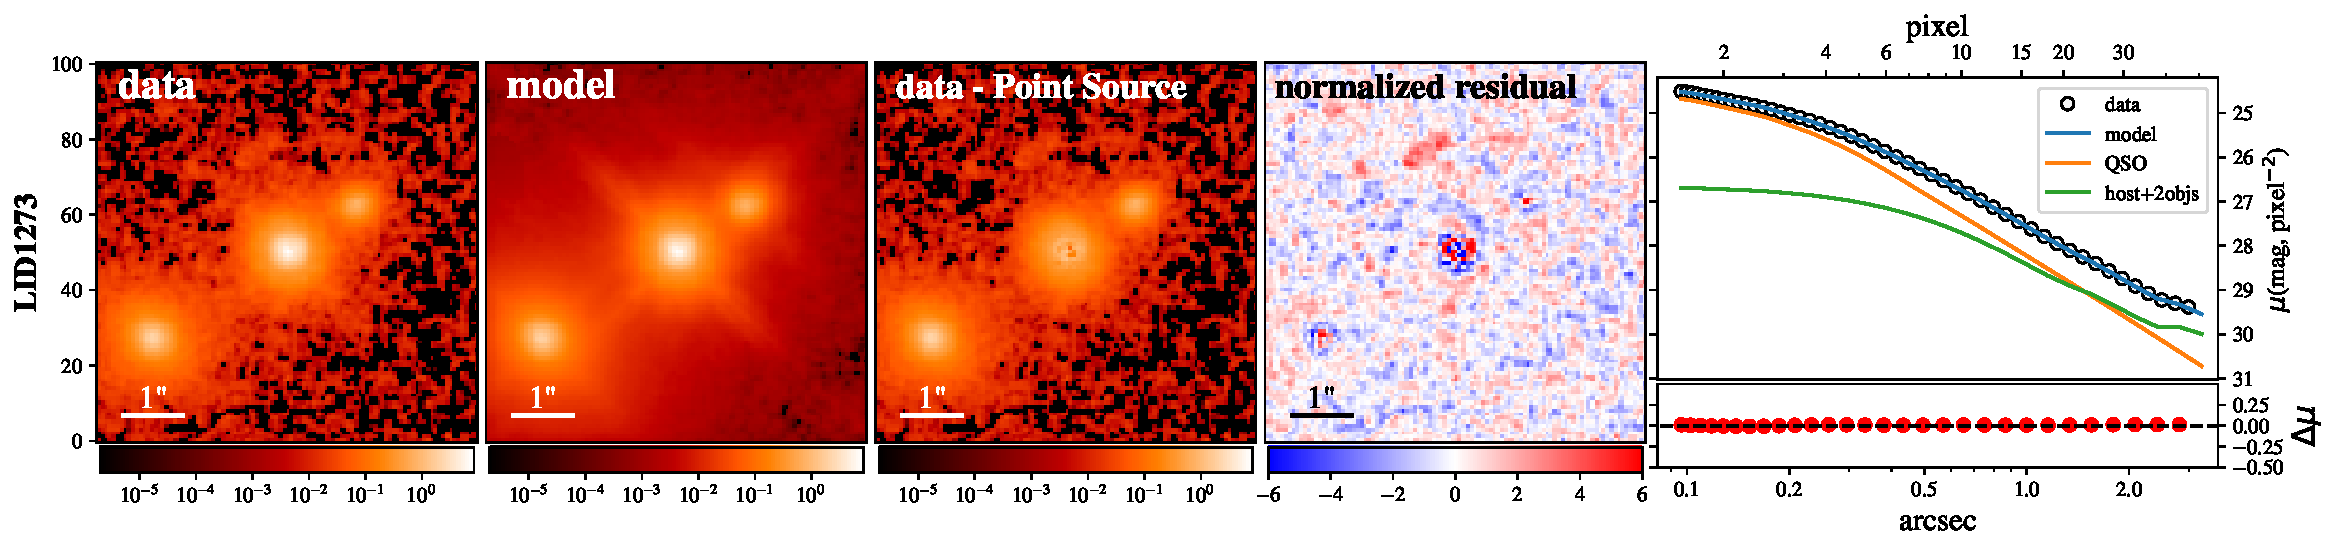
\includegraphics[height=0.25\textwidth]{fig/best_fit_LID1273_SB_profile.pdf}
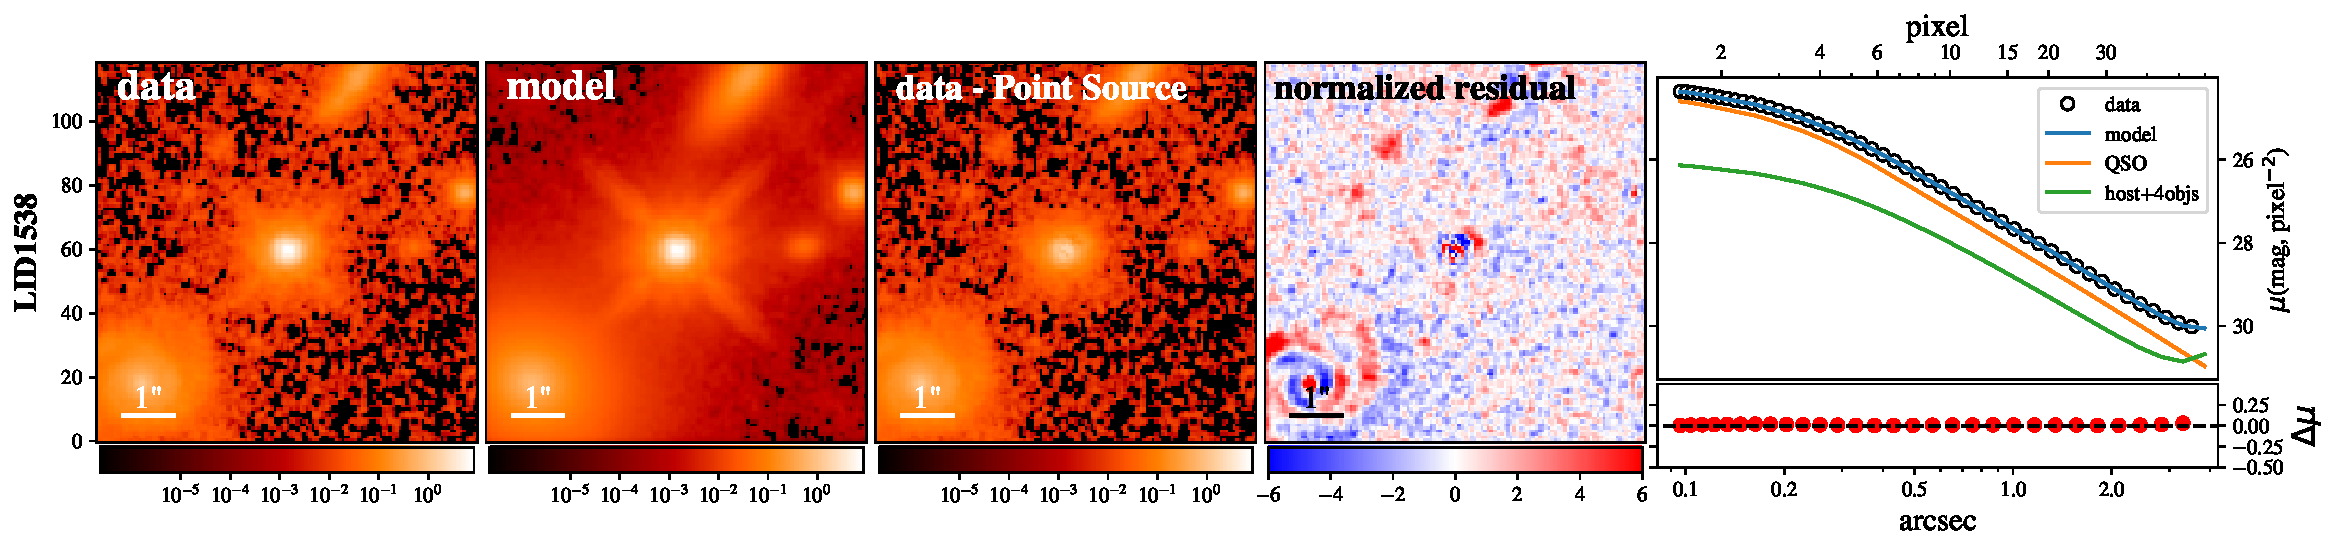
\includegraphics[height=0.25\textwidth]{fig/best_fit_LID1538_SB_profile.pdf}
}
%\figurenum{1}
%\caption{Continued.}
\end{figure*} 

\begin{figure*}
\centering
%\hspace{-5.5em}
{
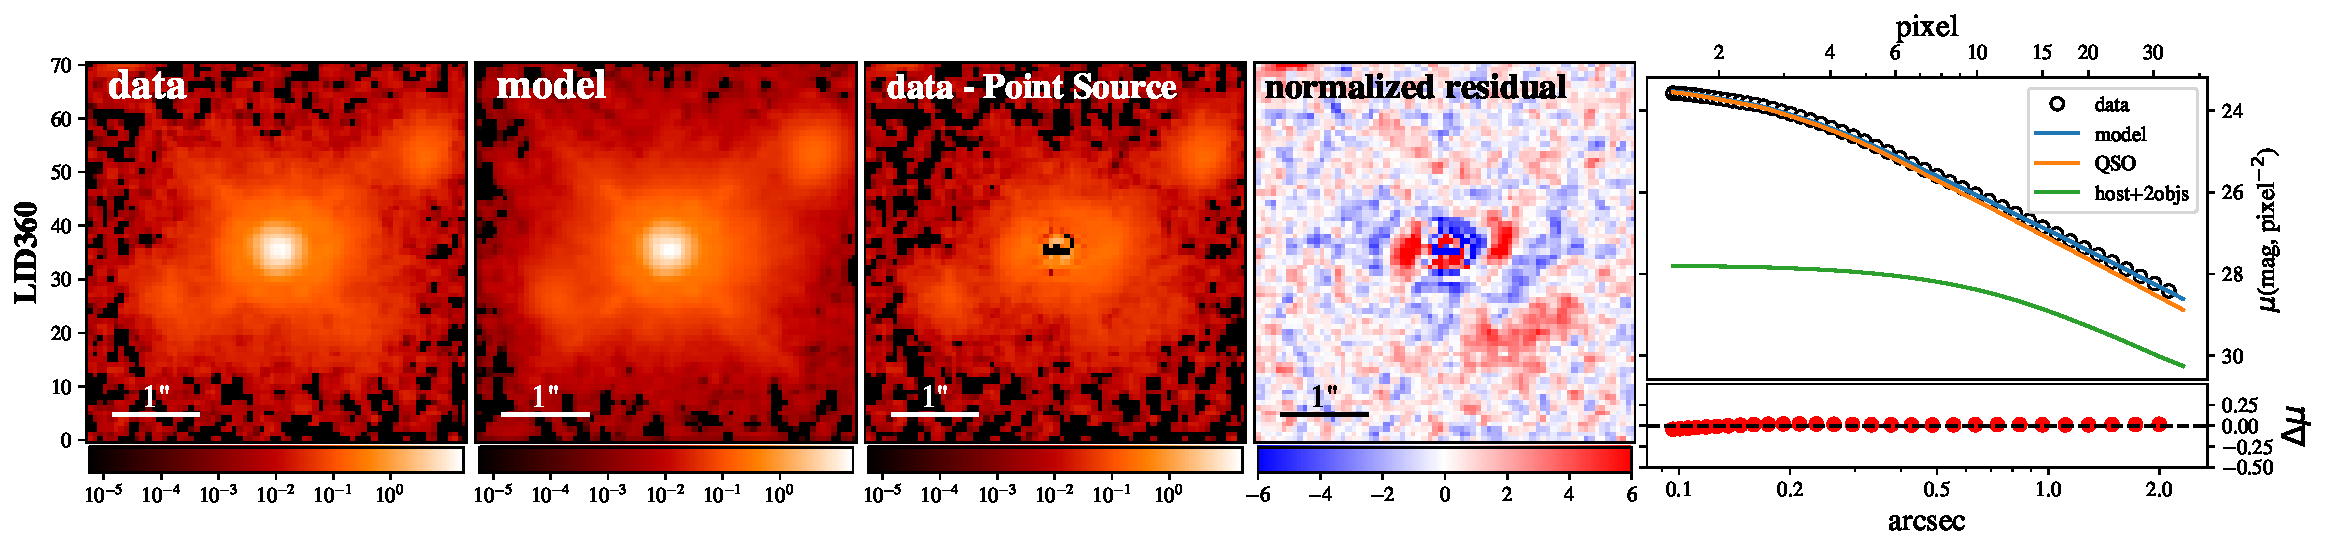
\includegraphics[height=0.25\textwidth]{fig/best_fit_LID360_SB_profile.pdf}
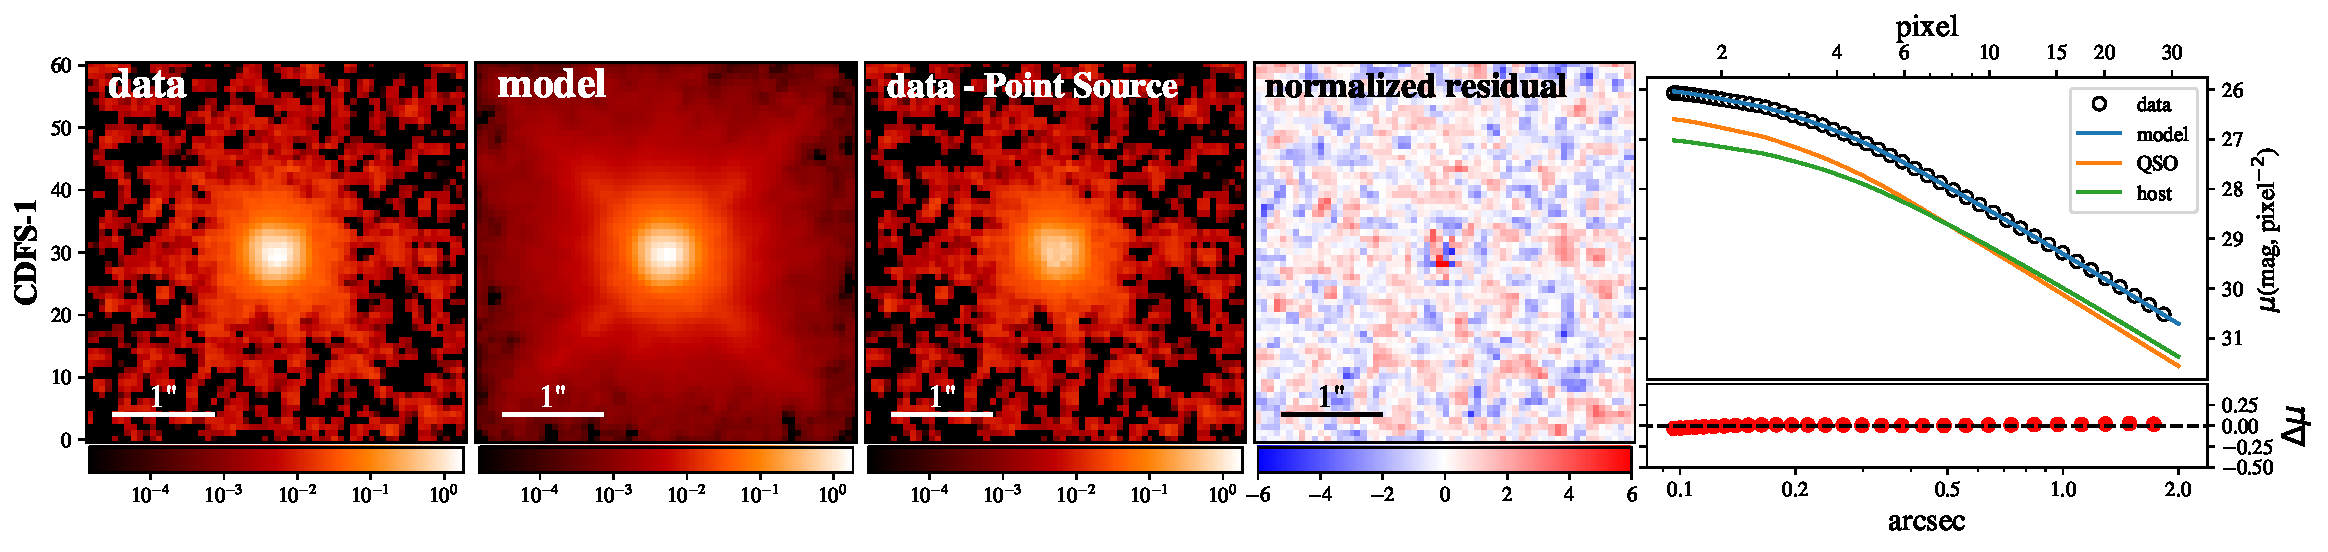
\includegraphics[height=0.25\textwidth]{fig/best_fit_CDFS-1_SB_profile.pdf}
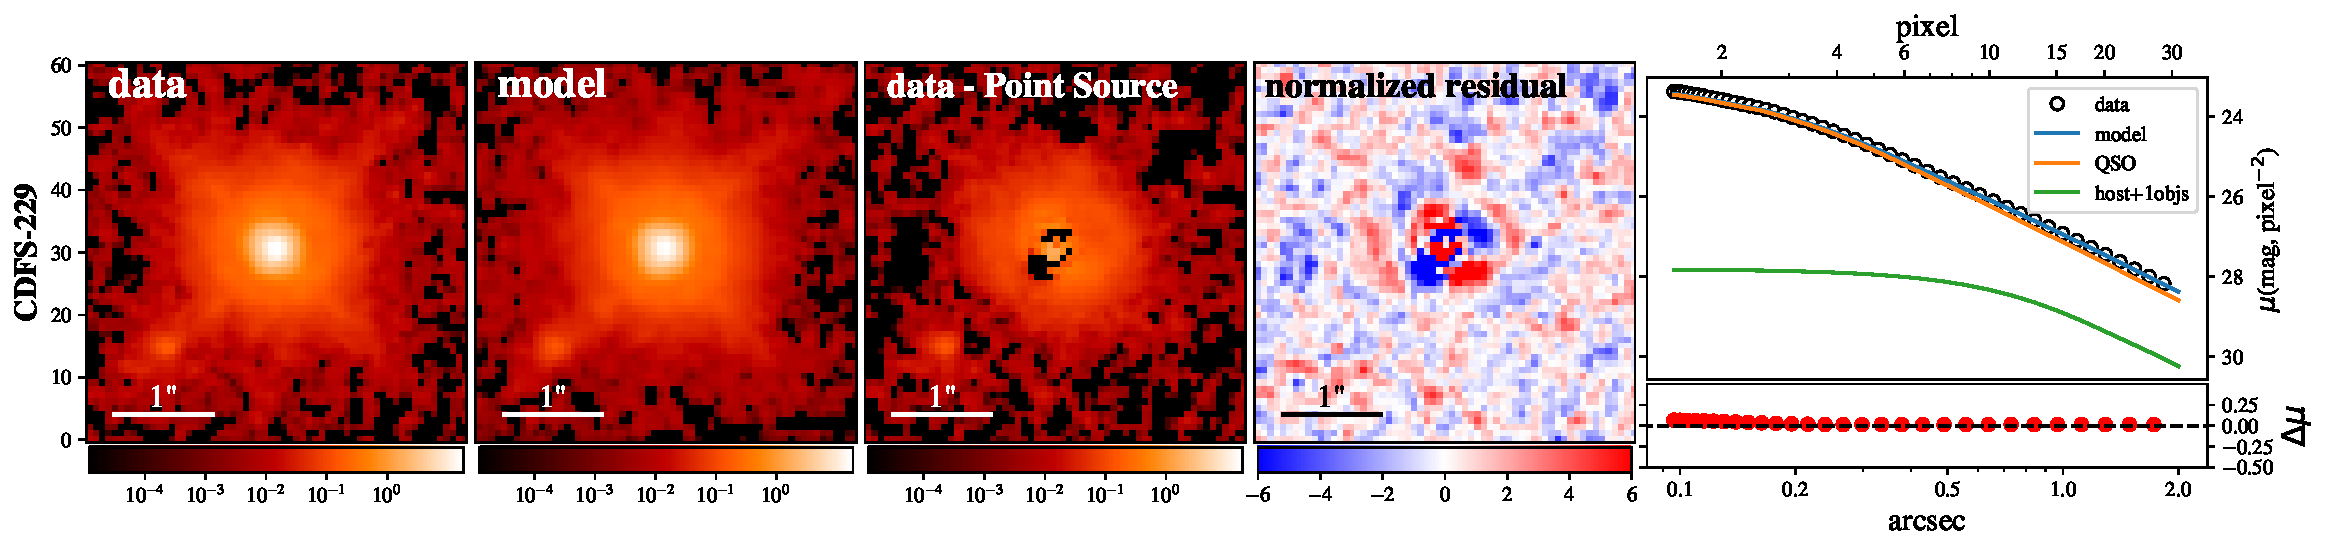
\includegraphics[height=0.25\textwidth]{fig/best_fit_CDFS-229_SB_profile.pdf}
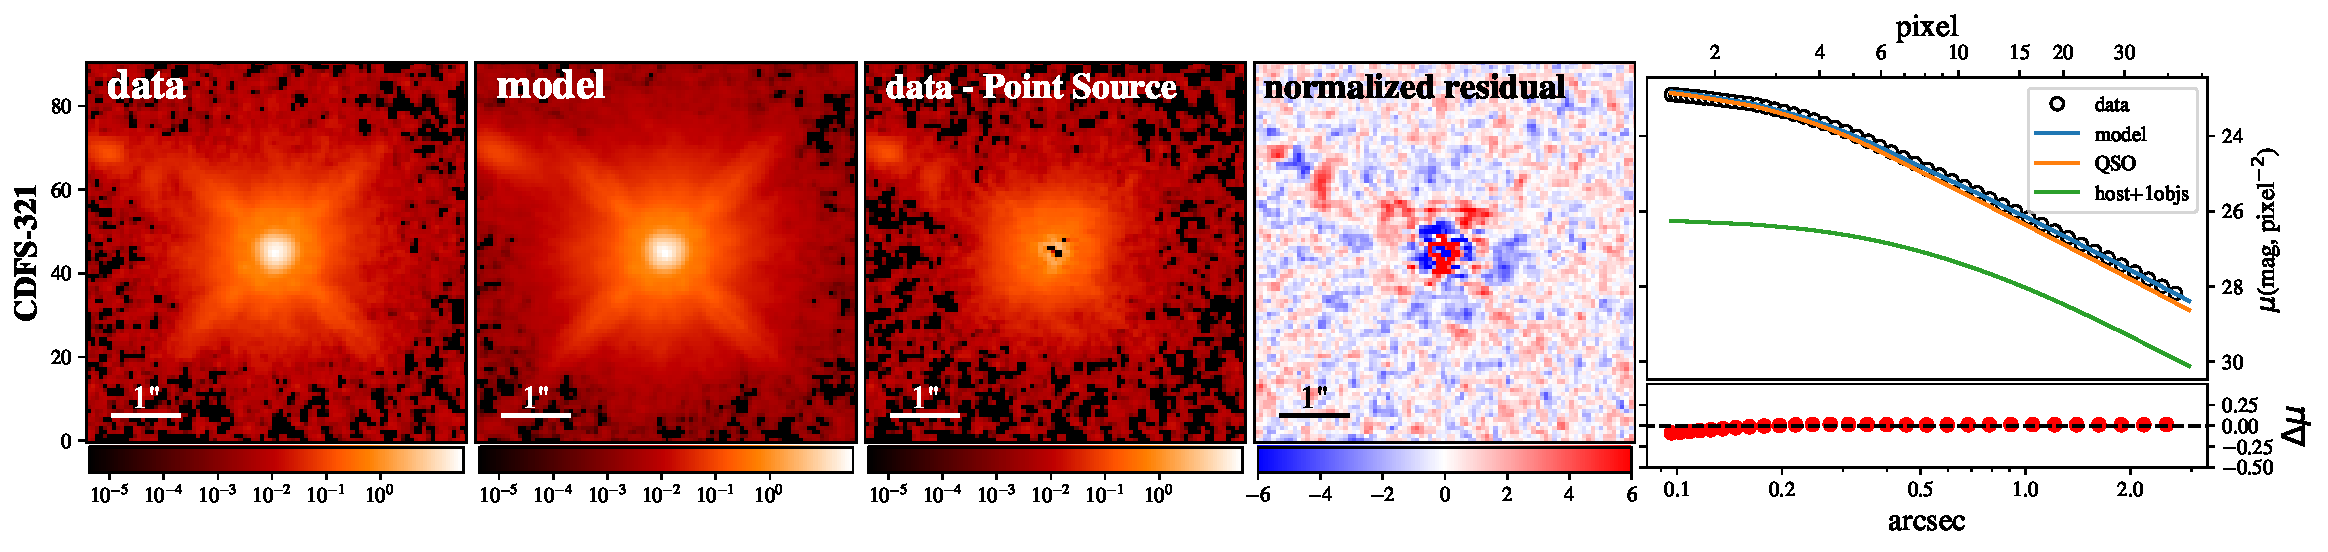
\includegraphics[height=0.25\textwidth]{fig/best_fit_CDFS-321_SB_profile.pdf}
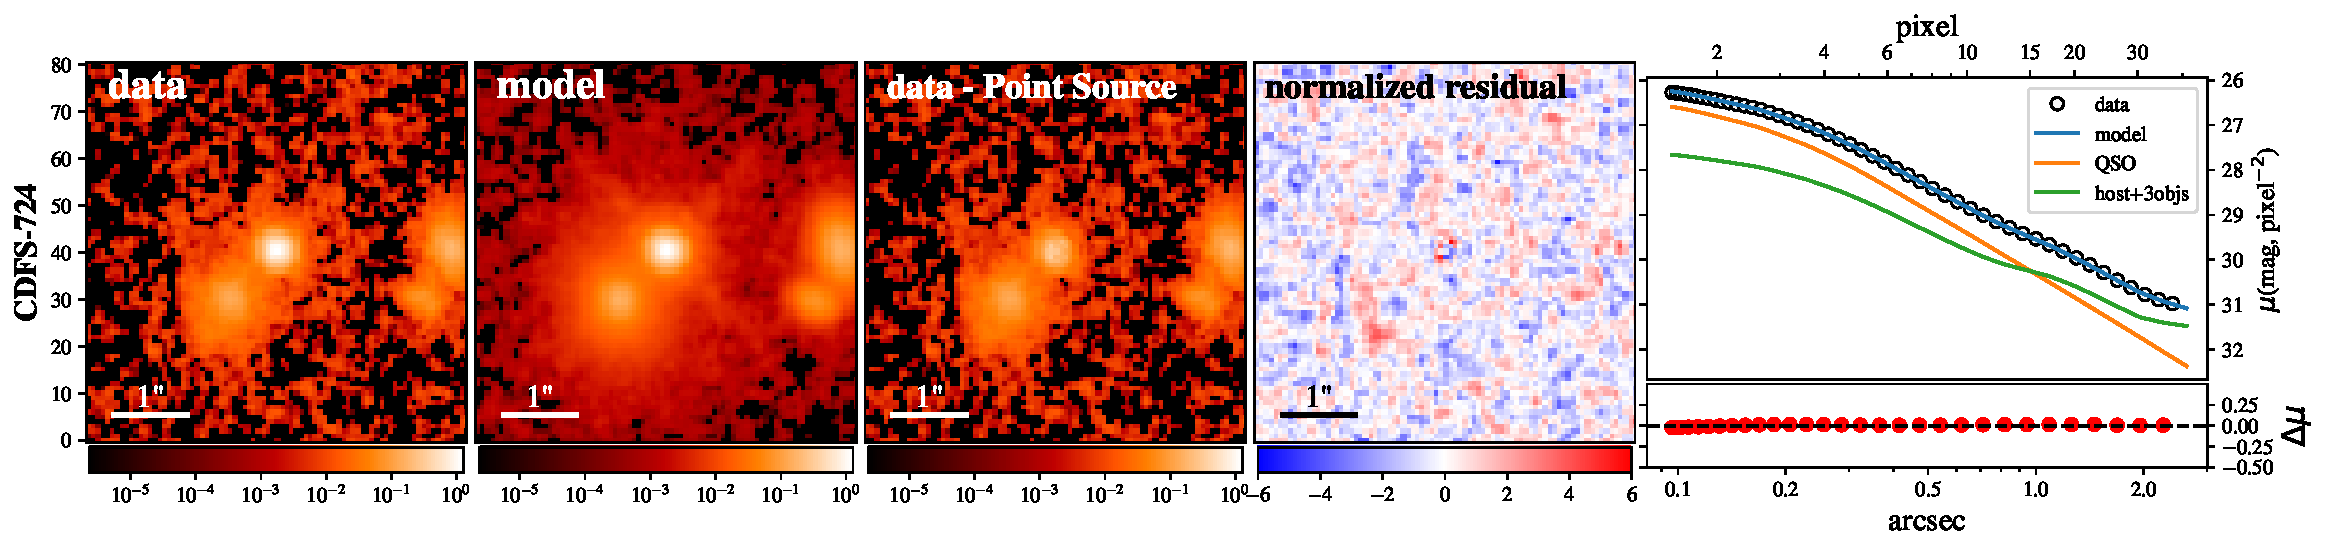
\includegraphics[height=0.25\textwidth]{fig/best_fit_CDFS-724_SB_profile.pdf}
}
%\figurenum{1}
%\caption{Continued.}
\end{figure*} 

\begin{figure*}
\centering
%\hspace{-5.5em}
{
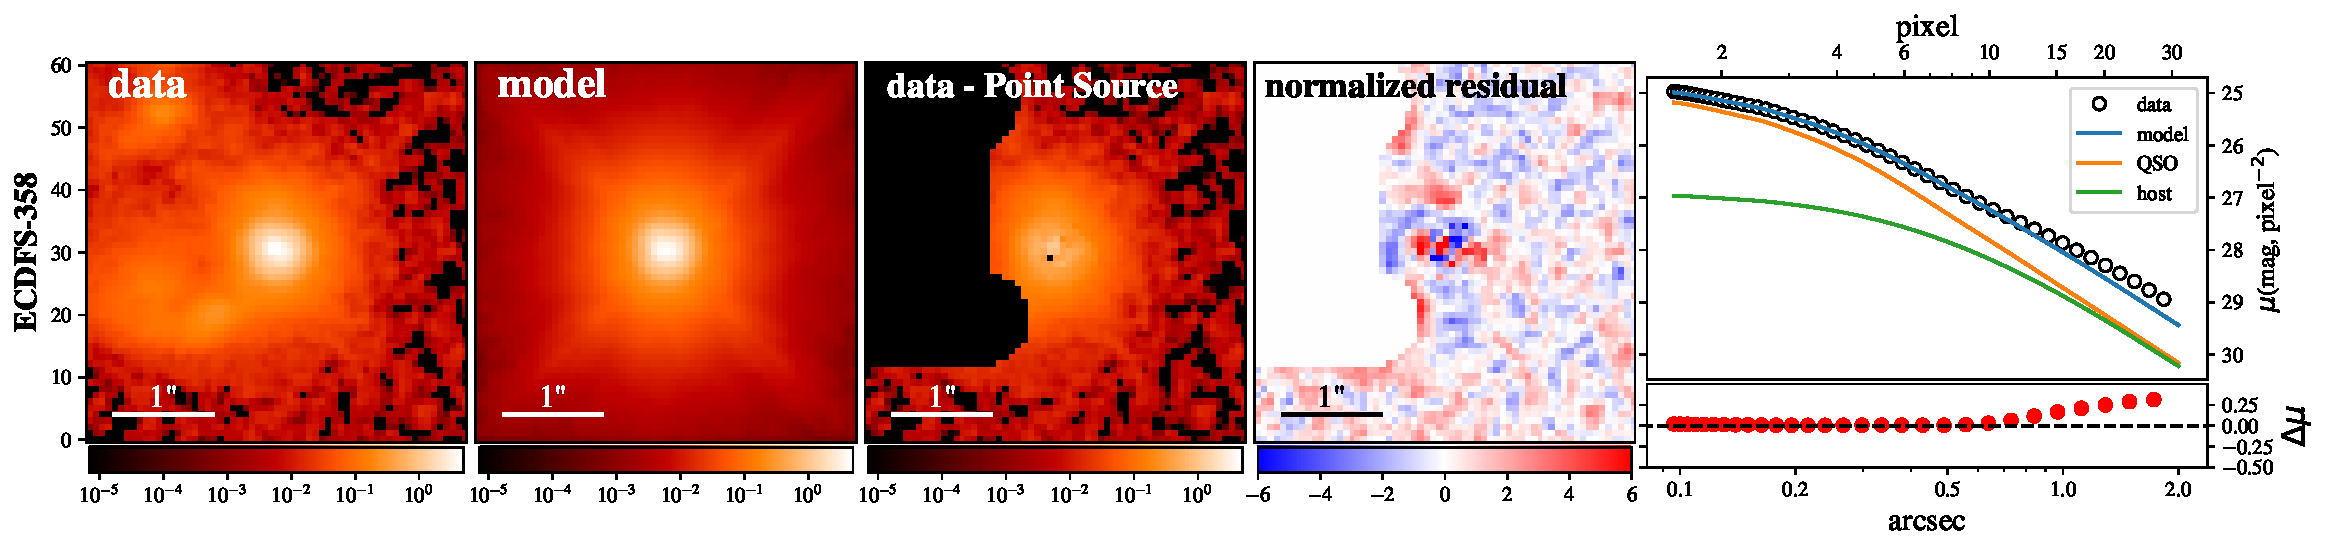
\includegraphics[height=0.25\textwidth]{fig/best_fit_ECDFS-358_SB_profile.pdf}
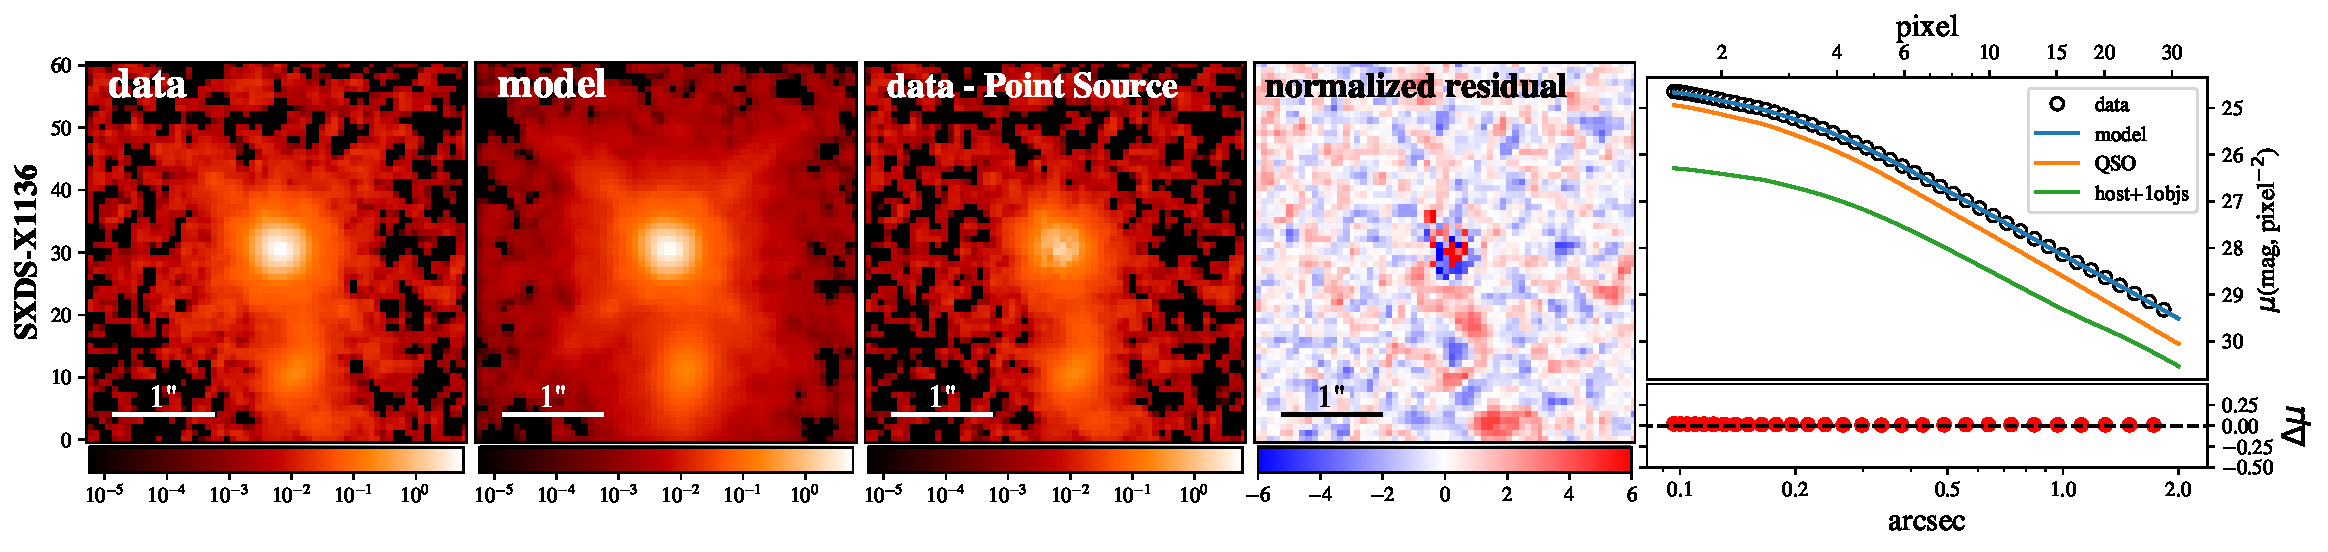
\includegraphics[height=0.25\textwidth]{fig/best_fit_SXDS-X1136_SB_profile.pdf}
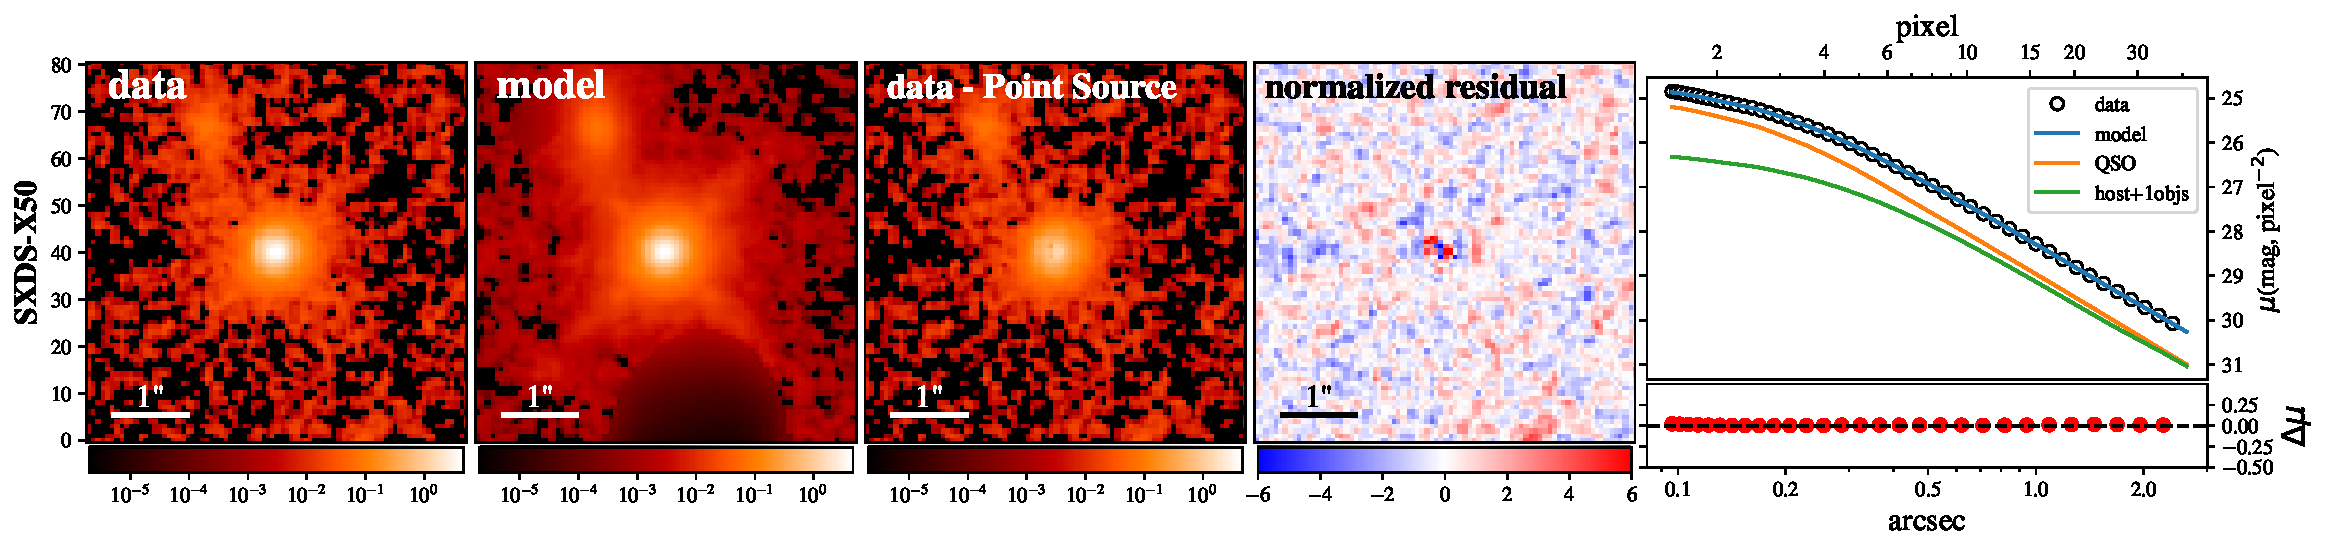
\includegraphics[height=0.25\textwidth]{fig/best_fit_SXDS-X50_SB_profile.pdf}
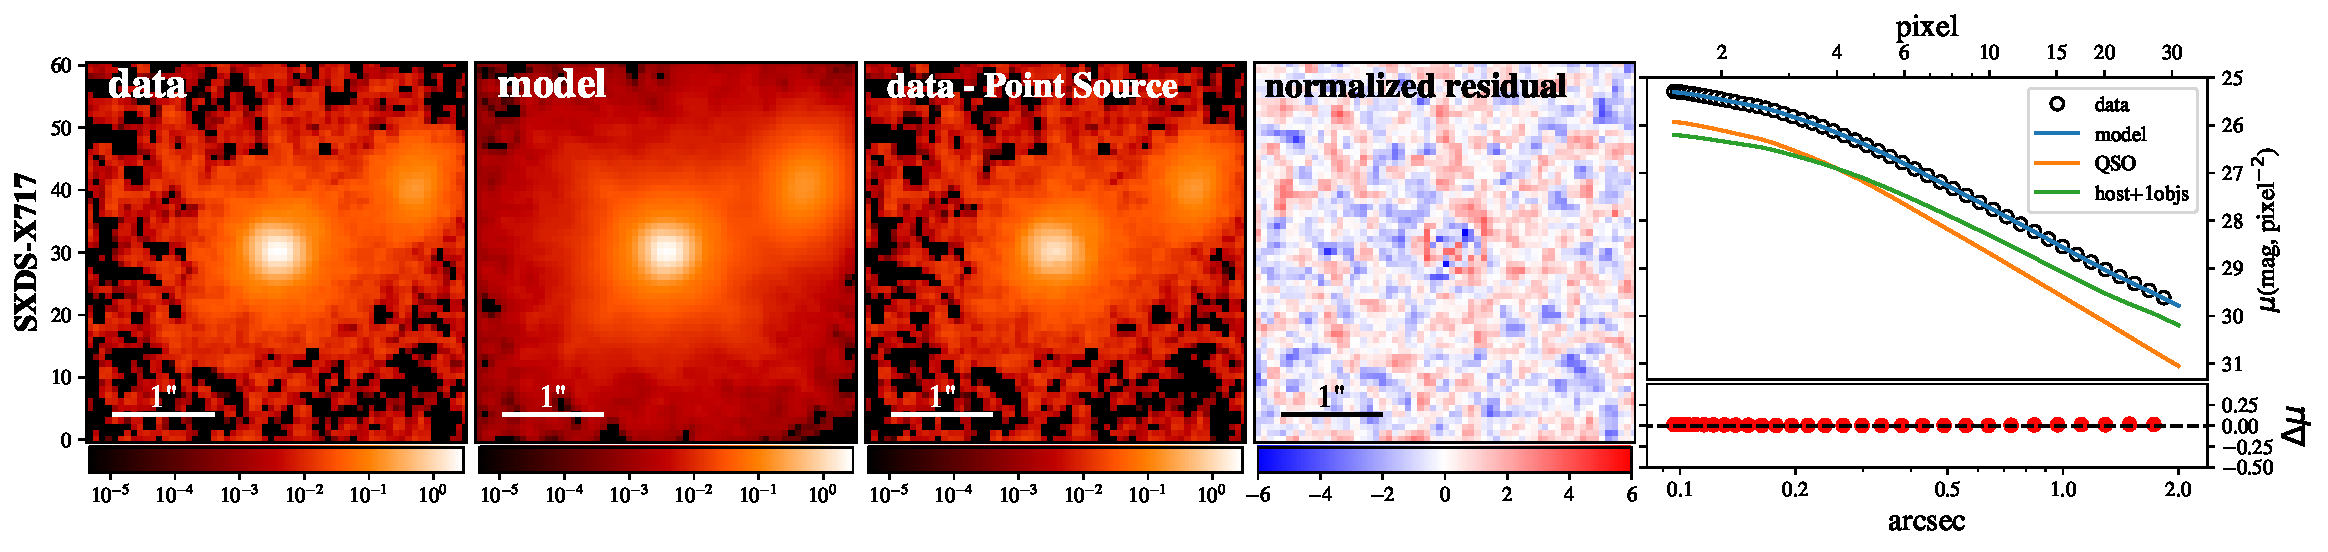
\includegraphics[height=0.25\textwidth]{fig/best_fit_SXDS-X717_SB_profile.pdf}
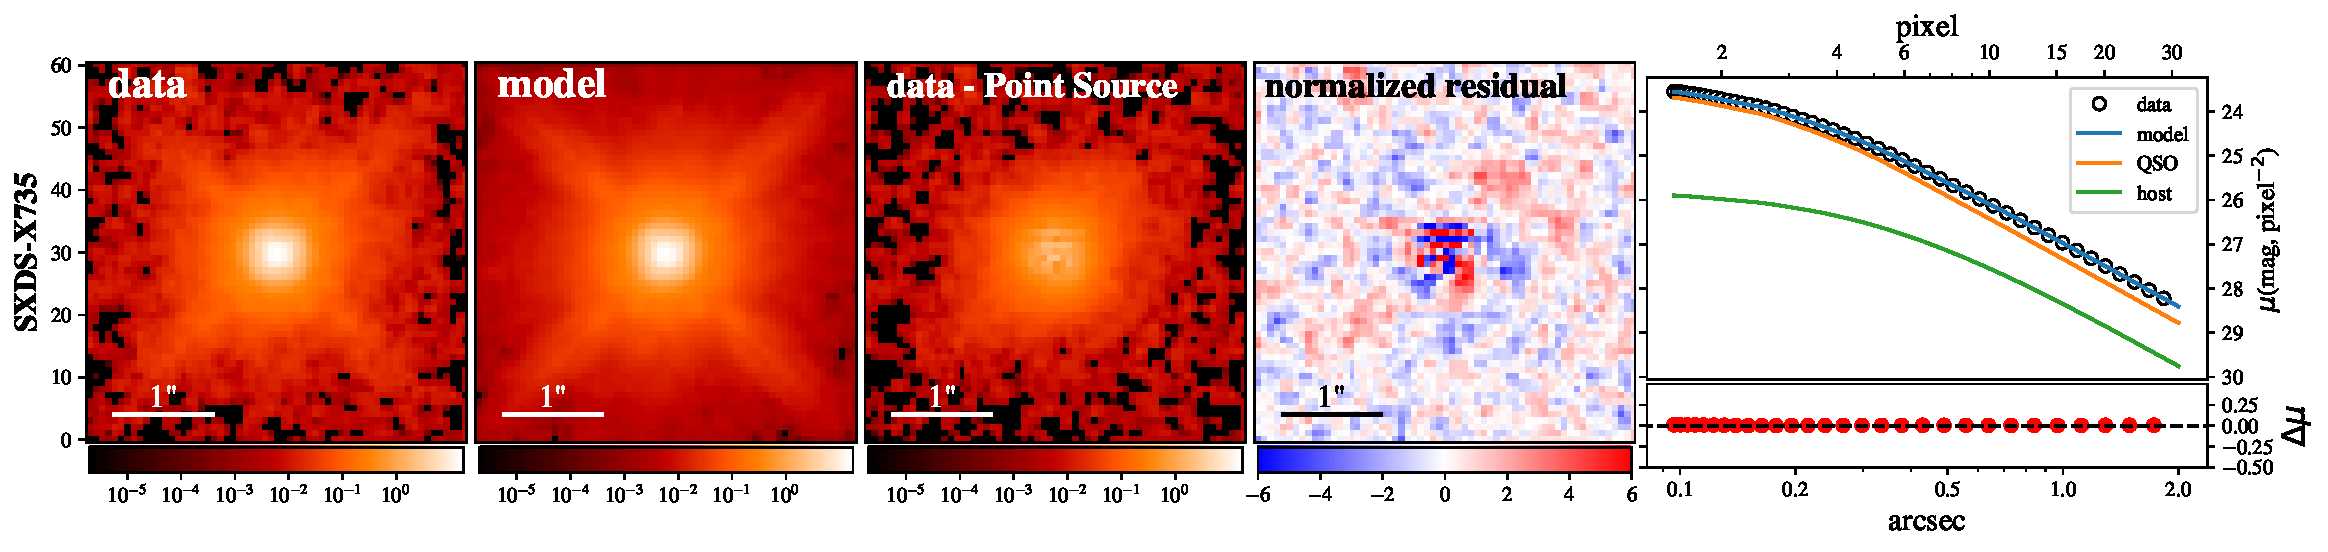
\includegraphics[height=0.25\textwidth]{fig/best_fit_SXDS-X735_SB_profile.pdf}
}
%\figurenum{1}
%\caption{Continued.}
\end{figure*} 

\begin{figure*}
\centering
%\hspace{-5.5em}
{
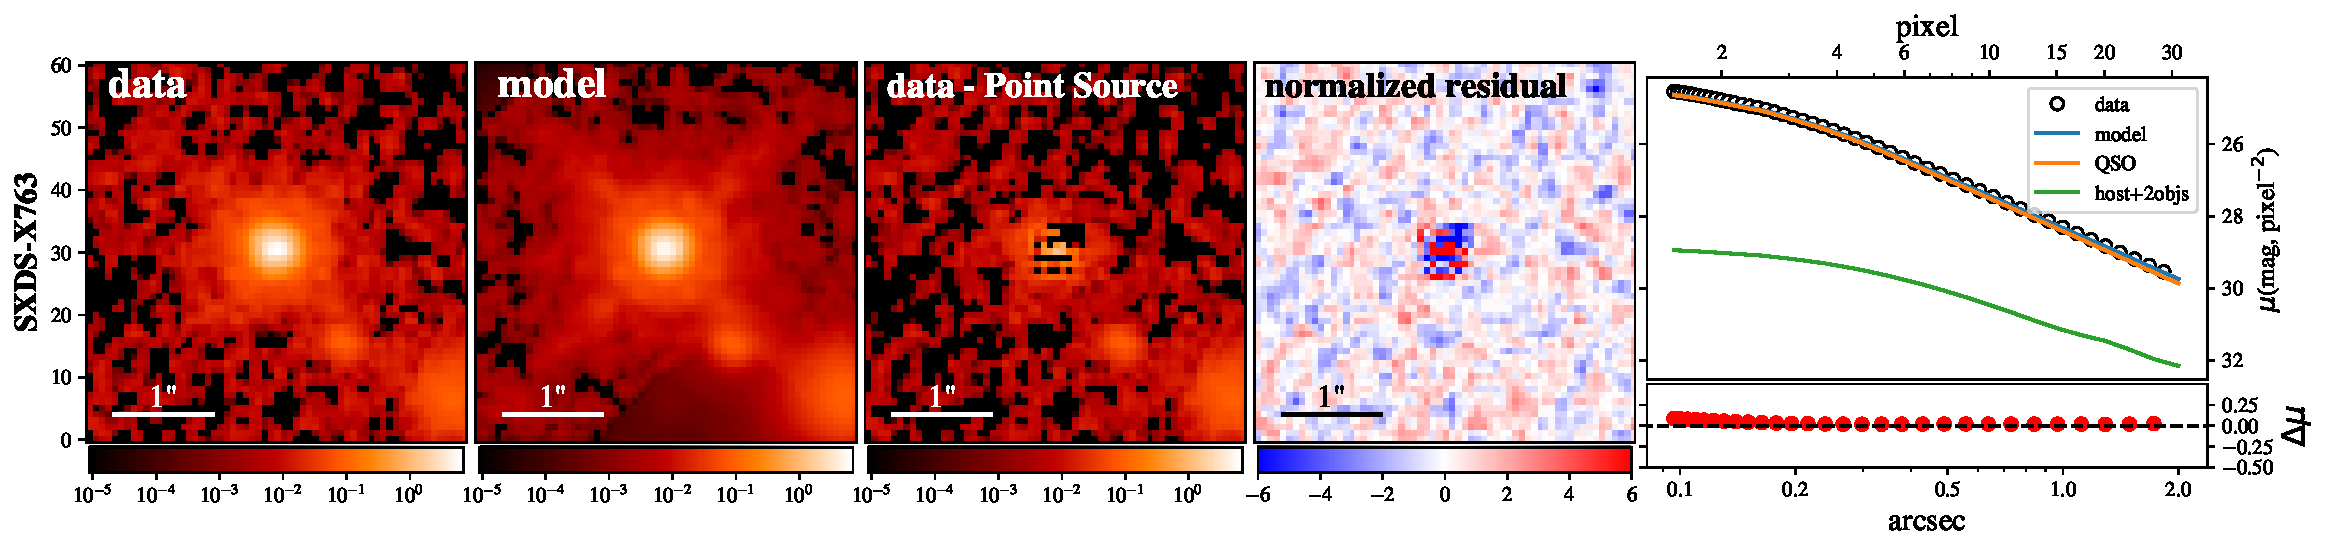
\includegraphics[height=0.25\textwidth]{fig/best_fit_SXDS-X763_SB_profile.pdf}
\includegraphics[height=0.25\textwidth]{fig/best_fit_SXDS-X969_SB_profile.pdf}
}
%\figurenum{1}
%\caption{Continued.}
\end{figure*} 

\end{document}